\documentclass[11pt,a4paper,dvipsnames,twosided]{article}
\usepackage[deliverable]{IOHKCoverPage}

% data for Deliverable header -- added by KH from an EU H2020 project template
\DeliverableNumber{SL-D5}
\DeliverableTitle{A Formal Specification of the Cardano Ledger}{Formal Cardano Ledger Spec.}
\DeliverableResponsible{Formal Methods Team}
\EditorName{Jared Corduan, \IOHK}
\Authors{Jared Corduan \quad \texttt{<jared.corduan@iohk.io>}
   \\[1em]
   Polina Vinogradova \quad \texttt{<polina.vinogradova@iohk.io>}
   \\[1em]
   Matthias G\"udemann \quad \texttt{<matthias.gudemann@iohk.io>}
}
\DueDate{15$^{\textrm{th}}$ October 2019}
\SubmissionDate{8th October 2019}{2019/10/08}
\LeaderName{Philipp Kant, \IOHK}
\InstitutionAddress{\IOHK}
\Version{1.0}
\Project{Shelley Ledger}
\DisseminationPU

\usepackage[margin=2.5cm]{geometry}
\usepackage{lscape}
\usepackage{iohk}
\usepackage{microtype}
\usepackage{mathpazo} % nice fonts
\usepackage{amsmath}
\usepackage{amssymb}
\usepackage{amsthm}
\usepackage{latexsym}
\usepackage{mathtools}
\usepackage{stmaryrd}
\usepackage{extarrows}
\usepackage{slashed}
\usepackage[unicode=true,pdftex,pdfa,colorlinks=true]{hyperref}
\usepackage{xcolor}
\usepackage[capitalise,noabbrev,nameinlink]{cleveref}
\usepackage{float}
\floatstyle{boxed}
\restylefloat{figure}
\usepackage{tikz}
\usepackage{booktabs}
\usepackage{enumerate}
\usepackage{listings}
%%
%% Package `semantic` can be used for writing inference rules.
%%
\usepackage{semantic}
%% Setup for the semantic package
\setpremisesspace{20pt}

\usepackage{tocloft}
\addtolength{\cftsubsecnumwidth}{5pt}

%%
%% Types
%%
\newcommand{\Nothing}{\ensuremath{\Diamond}}
\newcommand{\N}{\ensuremath{\mathbb{N}}}
\newcommand{\Bool}{\type{Bool}}
\newcommand{\Npos}{\ensuremath{\mathbb{N}^{>0}}}
\newcommand{\Z}{\ensuremath{\mathbb{Z}}}
\newcommand{\Q}{\ensuremath{\mathbb{Q}}}
\newcommand{\R}{\ensuremath{\mathbb{R}}}
\newcommand{\Rnn}{\ensuremath{\mathbb{R}^{\geq 0}}}
\newcommand{\Tx}{\type{Tx}}
\newcommand{\TxBody}{\type{TxBody}}
\newcommand{\TxWitness}{\type{TxWitness}}
\newcommand{\Ix}{\type{Ix}}
\newcommand{\TxId}{\type{TxId}}
\newcommand{\Addr}{\type{Addr}}
\newcommand{\UTxO}{\type{UTxO}}
\newcommand{\Wdrl}{\type{Wdrl}}
\newcommand{\Coin}{\type{Coin}}
\newcommand{\PParams}{\type{PParams}}
\newcommand{\PParamsUpdate}{\type{PParamsUpdate}}
\newcommand{\ProposedPPUpdates}{\type{ProposedPPUpdates}}
\newcommand{\Slot}{\type{Slot}}
\newcommand{\StabilityWindow}{\ensuremath{\mathsf{StabilityWindow}}}
\newcommand{\RandomnessStabilisationWindow}{\ensuremath{\mathsf{RandomnessStabilisationWindow}}}
\newcommand{\SlotsPerEpoch}{\mathsf{SlotsPerEpoch}}
\newcommand{\SlotsPerKESPeriod}{\mathsf{SlotsPerKESPeriod}}
\newcommand{\MaxMajorPV}{\mathsf{MaxMajorPV}}
\newcommand{\ActiveSlotCoeff}{\mathsf{ActiveSlotCoeff}}
\newcommand{\Network}{\mathsf{Network}}
\newcommand{\NetworkId}{\mathsf{NetworkId}}
\newcommand{\BlockNo}{\type{BlockNo}}
\newcommand{\MaxKESEvo}{\ensuremath{\mathsf{MaxKESEvo}}}
\newcommand{\Quorum}{\ensuremath{\mathsf{Quorum}}}
\newcommand{\MaxLovelaceSupply}{\ensuremath{\mathsf{MaxLovelaceSupply}}}
\newcommand{\Duration}{\type{Duration}}
\newcommand{\StakePools}{\type{StakePools}}
\newcommand{\Seed}{\type{Seed}}
\newcommand{\seedOp}{\star}
\newcommand{\Ppm}{\type{Ppm}}
\newcommand{\ProtVer}{\ensuremath{\type{ProtVer}}}
\newcommand{\Metadatum}{\ensuremath{\type{Metadatum}}}
\newcommand{\Metadata}{\ensuremath{\type{Metadata}}}
\newcommand{\MetadataHash}{\ensuremath{\type{MetadataHash}}}
\newcommand{\Update}{\type{Update}}
\newcommand{\GenesisDelegation}{\type{GenesisDelegation}}
\newcommand{\FutGenesisDelegation}{\type{FutGenesisDelegation}}

\newcommand{\DCert}{\type{DCert}}
\newcommand{\DCertRegKey}{\type{DCert_{regkey}}}
\newcommand{\DCertDeRegKey}{\type{DCert_{deregkey}}}
\newcommand{\DCertDeleg}{\type{DCert_{delegate}}}
\newcommand{\DCertRegPool}{\type{DCert_{regpool}}}
\newcommand{\DCertRetirePool}{\type{DCert_{retirepool}}}
\newcommand{\DCertGen}{\type{DCert_{genesis}}}
\newcommand{\DCertMir}{\type{DCert_{mir}}}
\newcommand{\PoolParam}{\type{PoolParam}}
\newcommand{\PoolMD}{\type{PoolMD}}
\newcommand{\MIRPot}{\type{MIRPot}}
\newcommand{\InstantaneousRewards}{\type{InstantaneousRewards}}
\newcommand{\ReservesMIR}{\type{ReservesMIR}}
\newcommand{\TreasuryMIR}{\type{TreasuryMIR}}
\newcommand{\URL}{\type{Url}}
\newcommand{\UTxOState}{\ensuremath{\type{UTxOState}}}
\newcommand{\ledgerState}{\ensuremath{\type{ledgerState}}}

\newcommand{\AddrRWD}{\type{Addr_{rwd}}}
\newcommand{\AddrB}{\type{Addr_{base}}}
\newcommand{\AddrP}{\type{Addr_{ptr}}}
\newcommand{\AddrE}{\type{Addr_{enterprise}}}
\newcommand{\AddrBS}{\type{Addr_{bootstrap}}}
\newcommand{\Ptr}{\type{Ptr}}
\newcommand{\DState}{\type{DState}}
\newcommand{\DWEnv}{\type{DWEnv}}
\newcommand{\DPSEnv}{\type{DPSEnv}}
\newcommand{\DPEnv}{\type{DPEnv}}
\newcommand{\DEnv}{\type{DEnv}}
\newcommand{\PEnv}{\type{PEnv}}
\newcommand{\DPState}{\type{DPState}}
\newcommand{\PState}{\type{PState}}
\newcommand{\DCertBody}{\type{DCertBody}}
\newcommand{\TData}{\type{TData}}
\newcommand{\DPoolReap}{\ensuremath{\type{poolreap}}}
\newcommand{\UPIState}{\type{UPIState}}
\newcommand{\UpdatePayload}{\type{UpdatePayload}}

% multi-signature
\newcommand{\StakeCredential}{\type{Credential}_{stake}}

\newcommand{\txwitsVKey}[1]{\fun{txwitsVKey}~\var{#1}}
\newcommand{\txwitsScript}[1]{\fun{txwitsScript}~\var{#1}}

\newcommand{\AddrVKey}{\type{Addr^{vkey}}}
\newcommand{\AddrRWDVKey}{\type{Addr_{rwd}^{vkey}}}
\newcommand{\AddrRWDScr}{\type{Addr_{rwd}^{script}}}
\newcommand{\AddrVKeyB}{\type{Addr^{vkey}_{base}}}
\newcommand{\AddrVKeyP}{\type{Addr^{vkey}_{ptr}}}
\newcommand{\AddrVKeyE}{\type{Addr^{vkey}_{enterprise}}}
\newcommand{\AddrVKeyBS}{\type{Addr^{vkey}_{bootstrap}}}
\newcommand{\AddrScr}{\type{Addr^{script}}}
\newcommand{\AddrScrBase}{\type{Addr_{base}^{script}}}
\newcommand{\AddrScrEnterprise}{\type{Addr_{enterprise}^{script}}}
\newcommand{\AddrScrPtr}{\type{Addr_{ptr}^{script}}}
\newcommand{\HashScr}{\type{ScriptHash}}
\newcommand{\Script}{\type{Script}}
\newcommand{\MSig}{\type{MSig}}
\newcommand{\Credential}{\type{Credential}}

%% Adding witnesses
\newcommand{\TxIn}{\type{TxIn}}
\newcommand{\TxOut}{\type{TxOut}}
\newcommand{\VKey}{\type{VKey}}
\newcommand{\VKeyEv}{\type{VKey_{ev}}}
\newcommand{\VKeyGen}{\type{VKey_G}}
\newcommand{\SKey}{\type{SKey}}
\newcommand{\SKeyEv}{\type{SKey_{ev}}}
\newcommand{\KeyHash}{\type{KeyHash}}
\newcommand{\KeyHashGen}{\type{KeyHash_G}}
\newcommand{\KeyPair}{\type{KeyPair}}
\newcommand{\KeyPairEv}{\type{KeyPair_{ev}}}
\newcommand{\Sig}{\type{Sig}}
\newcommand{\Data}{\type{Data}}
\newcommand{\Ser}{\type{Ser}}
%% Adding delegation
\newcommand{\Epoch}{\type{Epoch}}
\newcommand{\KESPeriod}{\type{KESPeriod}}
%% Blockchain
\newcommand{\Acnt}{\type{Acnt}}
\newcommand{\Gkeys}{\var{G_{keys}}}
\newcommand{\Block}{\type{Block}}
\newcommand{\SlotId}{\type{SlotId}}
\newcommand{\PPUpdateState}{\type{PPUpdateState}}
\newcommand{\PPUpdateEnv}{\type{PPUpdateEnv}}
\newcommand{\UTxOEnv}{\type{UTxOEnv}}
\newcommand{\CEEnv}{\type{CEEnv}}
\newcommand{\CEState}{\type{CEState}}
\newcommand{\BDEnv}{\type{BDEnv}}
\newcommand{\BDState}{\type{BDState}}
\newcommand{\LEnv}{\type{LEnv}}
\newcommand{\LState}{\type{LState}}

\newcommand{\Proof}{\type{Proof}}
\newcommand{\Seedl}{\mathsf{Seed}_\ell}
\newcommand{\Seede}{\mathsf{Seed}_\eta}
\newcommand{\slotToSeed}[1]{\fun{slotToSeed}~ \var{#1}}
\newcommand{\prevHashToNonce}[1]{\fun{prevHashToNonce}~ \var{#1}}
\newcommand{\isOverlaySlot}[3]{\fun{isOverlaySlot}~\var{#1}~\var{#2}~\var{#3}}
\newcommand{\classifyOverlaySlot}[5]{\fun{classifyOverlaySlot}~\var{#1}~\var{#2}~\var{#3}~\var{#4}~\var{#5}}

\newcommand{\T}{\type{T}}
\newcommand{\vrf}[3]{\fun{vrf}_{#1} ~ #2 ~ #3}
\newcommand{\verifyVrf}[4]{\fun{verifyVrf}_{#1} ~ #2 ~ #3 ~#4}

\newcommand{\HashHeader}{\type{HashHeader}}
\newcommand{\HashBBody}{\type{HashBBody}}
\newcommand{\bhHash}[1]{\fun{bhHash}~ \var{#1}}
\newcommand{\bHeaderSize}[1]{\fun{bHeaderSize}~ \var{#1}}
\newcommand{\bSize}[1]{\fun{bSize}~ \var{#1}}
\newcommand{\bBodySize}[1]{\fun{bBodySize}~ \var{#1}}
\newcommand{\OCert}{\type{OCert}}
\newcommand{\BHeader}{\type{BHeader}}
\newcommand{\BHBody}{\type{BHBody}}

\newcommand{\bheader}[1]{\fun{bheader}~\var{#1}}
\newcommand{\hsig}[1]{\fun{hsig}~\var{#1}}
\newcommand{\bprev}[1]{\fun{bprev}~\var{#1}}
\newcommand{\bhash}[1]{\fun{bhash}~\var{#1}}
\newcommand{\bvkcold}[1]{\fun{bvkcold}~\var{#1}}
\newcommand{\bseedl}[1]{\fun{bseed}_{\ell}~\var{#1}}
\newcommand{\bprfn}[1]{\fun{bprf}_{n}~\var{#1}}
\newcommand{\bseedn}[1]{\fun{bseed}_{n}~\var{#1}}
\newcommand{\bprfl}[1]{\fun{bprf}_{\ell}~\var{#1}}
\newcommand{\bocert}[1]{\fun{bocert}~\var{#1}}
\newcommand{\bnonce}[1]{\fun{bnonce}~\var{#1}}
\newcommand{\bleader}[1]{\fun{bleader}~\var{#1}}
\newcommand{\hBbsize}[1]{\fun{hBbsize}~\var{#1}}
\newcommand{\bbodyhash}[1]{\fun{bbodyhash}~\var{#1}}
\newcommand{\overlaySchedule}[3]{\fun{overlaySchedule}~\var{#1}~\var{#2}~\var{#3}}

\newcommand{\OCertEnv}{\type{OCertEnv}}
\newcommand{\PrtclState}{\type{PrtclState}}
\newcommand{\PrtclEnv}{\type{PrtclEnv}}
\newcommand{\OverlayEnv}{\type{OverlayEnv}}
\newcommand{\VRFState}{\type{VRFState}}
\newcommand{\TickNonceState}{\type{TickNonceState}}
\newcommand{\TickNonceEnv}{\type{TickNonceEnv}}
\newcommand{\NewEpochState}{\type{NewEpochState}}
\newcommand{\UpdateNonceState}{\type{UpdateNonceState}}
\newcommand{\UpdateNonceEnv}{\type{UpdateNonceEnv}}
\newcommand{\PoolDistr}{\type{PoolDistr}}
\newcommand{\BBodyEnv}{\type{BBodyEnv}}
\newcommand{\BBodyState}{\type{BBodyState}}
\newcommand{\RUpdEnv}{\type{RUpdEnv}}
\newcommand{\ChainEnv}{\type{ChainEnv}}
\newcommand{\ChainState}{\type{ChainState}}
\newcommand{\ChainSig}{\type{ChainSig}}
\newcommand{\LastAppliedBlock}{\type{LastAppliedBlock}}
\newcommand{\lastAppliedHash}[1]{\fun{lastAppliedHash}~\var{#1}}


%%
%% Functions
%%
\newcommand{\txins}[1]{\fun{txins}~ \var{#1}}
\newcommand{\txouts}[1]{\fun{txouts}~ \var{#1}}
\newcommand{\txcerts}[1]{\fun{txcerts}~ \var{#1}}
\newcommand{\txid}[1]{\fun{txid}~ \var{#1}}
\newcommand{\outs}[1]{\fun{outs}~ \var{#1}}
\newcommand{\values}[1]{\fun{values}~ #1}
\newcommand{\ubalance}[1]{\fun{ubalance}~ \var{#1}}
\newcommand{\txttl}[1]{\fun{txttl}~ \var{#1}}
\newcommand{\firstSlot}[1]{\fun{firstSlot}~ \var{#1}}
\newcommand{\totalDeposits}[3]{\fun{totalDeposits}~ \var{#1} ~ \var{#2} ~ \var{#3}}
\newcommand{\keyRefund}[6]{\fun{keyRefund}~ {#1}~{#2}~{#3}~\var{#4}~\var{#5}~\var{#6}}
\newcommand{\refund}[4]{\fun{refund}~ \var{#1}~ \var{#2}~ {#3}~ {#4}}
\newcommand{\keyRefunds}[2]{\fun{keyRefunds}~ \var{#1}~ \var{#2}}
\newcommand{\consumed}[2]{\fun{consumed}~ \var{#1}~ \var{#2}}
\newcommand{\produced}[2]{\fun{produced}~ \var{#1}~ \var{#2}}
\newcommand{\applyFun}[2]{\fun{#1}~\var{#2}}

\newcommand{\RegKey}[1]{\textsc{RegKey}(#1)}
\newcommand{\DeregKey}[1]{\textsc{DeregKey}(#1)}
\newcommand{\Delegate}[1]{\textsc{Delegate}(#1)}
\newcommand{\RegPool}[1]{\textsc{RegPool}(#1)}
\newcommand{\RetirePool}[1]{\textsc{RetirePool}(#1)}
\newcommand{\cwitness}[1]{\fun{cwitness}~ \var{#1}}
\newcommand{\dpool}[1]{\fun{dpool}~ \var{#1}}
\newcommand{\poolParam}[1]{\fun{poolParam}~ \var{#1}}
\newcommand{\retire}[1]{\fun{retire}~ \var{#1}}
\newcommand{\addrRw}[1]{\fun{addr_{rwd}}~ \var{#1}}
\newcommand{\epoch}[1]{\fun{epoch}~\var{#1}}
\newcommand{\kesPeriod}[1]{\fun{kesPeriod}~\var{#1}}

%% UTxO witnesses
\newcommand{\inputs}[1]{\fun{inputs}~ \var{#1}}
\newcommand{\txwits}[1]{\fun{txwits}~ \var{#1}}
\newcommand{\verify}[3]{\fun{verify} ~ #1 ~ #2 ~ #3}
\newcommand{\sign}[2]{\fun{sign} ~ #1 ~ #2}
\newcommand{\verifyEv}[4]{\fun{verify_{ev}} ~ #1 ~ #2 ~ #3 ~ #4}
\newcommand{\signEv}[3]{\fun{sign_{ev}} ~ #1 ~ #2 ~ #3}
\newcommand{\serialised}[1]{\llbracket \var{#1} \rrbracket}
\newcommand{\hashKey}[1]{\fun{hashKey}~ \var{#1}}
\newcommand{\txbody}[1]{\fun{txbody}~ \var{#1}}
\newcommand{\txfee}[1]{\fun{txfee}~ \var{#1}}
\newcommand{\txwdrls}[1]{\fun{txwdrls}~ \var{#1}}
\newcommand{\minfee}[2]{\fun{minfee}~ \var{#1}~ \var{#2}}
\newcommand{\slotminus}[2]{\var{#1}~-_{s}~\var{#2}}
\DeclarePairedDelimiter\floor{\lfloor}{\rfloor}
% wildcard parameter
\newcommand{\wcard}[0]{\rule[-.5mm]{2mm}{.2mm}}
%% Adding ledgers...
\newcommand{\utxo}[1]{\fun{utxo}~ #1}
%% Delegation
\newcommand{\delegatesName}{\fun{delegates}}
\newcommand{\delegates}[3]{\delegatesName~#1~#2~#3}
\newcommand{\dwho}[1]{\fun{dwho}~\var{#1}}
\newcommand{\depoch}[1]{\fun{depoch}~\var{#1}}
\newcommand{\dval}{\ensuremath{d_{\mathsf{val}}}}
%% Delegation witnesses
\newcommand{\dbody}[1]{\fun{dbody}~\var{#1}}
\newcommand{\dwit}[1]{\fun{dwit}~\var{#1}}
%% Blockchain
\newcommand{\bwit}[1]{\fun{bwit}~\var{#1}}
\newcommand{\bslot}[1]{\fun{bslot}~\var{#1}}
\newcommand{\bblockno}[1]{\fun{bblockno}~\var{#1}}
\newcommand{\bbody}[1]{\fun{bbody}~\var{#1}}
\newcommand{\bhbody}[1]{\fun{bhbody}~\var{#1}}
\newcommand{\bdlgs}[1]{\fun{bdlgs}~\var{#1}}
%% ledgerstate constants
\newcommand{\genesisId}{\ensuremath{Genesis_{Id}}}
\newcommand{\genesisTxOut}{\ensuremath{Genesis_{Out}}}
\newcommand{\genesisUTxO}{\ensuremath{Genesis_{UTxO}}}
\newcommand{\genesisUTxOState}{(\genesisUTxO,\wcard,\wcard,\wcard)}
\newcommand{\emax}{\ensuremath{\mathsf{E_{max}}}}

\newcommand{\unitInterval}{\ensuremath{[0,~1]}}
\newcommand{\unitIntervalNonNull}{\ensuremath{(0,~1]}}
\newcommand{\nonnegReals}{\ensuremath{[0,~\infty)}}
\newcommand{\posReals}{\ensuremath{(0,~\infty)}}

\theoremstyle{definition}
\newtheorem{definition}{Definition}[section]
\newtheorem{lemma}[definition]{Lemma}
\newtheorem{theorem}[definition]{Theorem}
\newtheorem{property}{Property}[section]

\newcommand{\leteq}{\ensuremath{\mathrel{\mathop:}=}}

\begin{document}

\hypersetup{
  pdftitle={A Formal Specification of the Cardano Ledger},
  breaklinks=true,
  bookmarks=true,
  colorlinks=false,
  linkcolor={blue},
  citecolor={blue},
  urlcolor={blue},
  linkbordercolor={white},
  citebordercolor={white},
  urlbordercolor={white}
}

  \cleardoublepage%
  \tableofcontents%

  \listoffigures%
  \clearpage%

  \begin{changelog}
        \change{2019/10/08}{Jared Corduan, Polina Vinogradova and Matthias G\"udemann}{FM (IOHK)}{Initial version (0.1).}
        \change{2019/10/08}{Kevin Hammond}{FM (IOHK)}{Added cover page.}
        \change{2020/11/17}{Jared Corduan}{FM (IOHK)}
          {Removed unused deliverable outline image,
           set version to 1.0,
           and changed the reward calculation so that $\eta$
             takes $d$ into account.}
        \change{2021/05/17}{Jared Corduan}{FM (IOHK)}{Added Example Illustration.}
        \change{2021/06/14}{Jared Corduan}{FM (IOHK)}
          {Added an errata section,
           fixed a typo in leader check and in the LEDGERS rule index,
           and synced the reward calculation with the implementation}
        \change{2021/06/17}{Jared Corduan}{FM (IOHK)}
          {Allow the pool influence parameter $a_0$ to be zero,
          remove all mentions of deposit decay, sync varibale names with code.}
        \change{2021/08/27}{Jared Corduan}{FM (IOHK)}{Fixed definitions in the header-only validation properties.
          CHAIN transition did not need to use previous protocol parameters.}
        \change{2021/10/08}{Jared Corduan}{FM (IOHK)}{The function createRUpd
          should get the pool parameters from the go snapshot.
          The TICKN rule was missing from the dependency diagram.}
        \change{2021/11/08}{Jared Corduan}{FM (IOHK)}{Fixed typo in the description of variable length encodings.}
        \change{2021/12/13}{Jared Corduan}{FM (IOHK)}{Re-wrote the MIR transitions to be more compact.}
      \end{changelog}
      \clearpage%
\renewcommand{\thepage}{\arabic{page}}
\setcounter{page}{1}

\title{A Formal Specification of the Cardano Ledger}

\author{Jared Corduan  \\ {\small \texttt{jared.corduan@iohk.io}} \\
   \and Polina Vinogradova \\ {\small \texttt{polina.vinogradova@iohk.io}} \\
   \and Matthias G\"udemann  \\ {\small \texttt{matthias.gudemann@iohk.io}}}

%\date{}

\maketitle

\begin{abstract}
This document provides a formal specification of the Cardano ledger for use in the upcoming Shelley implementation.
It is intended to underpin a Haskell executable specification that will be the basis of the initial
Shelley release, and represents a core design and quality assurance document.
It will be used to define properties and tests, and to provide the basis for strong formal assurance
using mathematical proof techniques.
The document defines the rules for extending the ledger with transactions
that will affect both UTxO and stake delegation.
Key properties that have been identified include the preservation of balances, absence of double spend, stakepool registration,
and reward splitting.
\end{abstract}

\section*{List of Contributors}
\label{acknowledgements}

Nicol\'as Arqueros,
Dan Bornside,
Nicholas Clarke,
Duncan Coutts,
Ruslan Dudin,
Sebastien Guillemot,
Kevin Hammond,
Vincent Hanquez,
Ru Horlick,
Michael Hueschen,
Christian Lindgren,
Yun Lu,
Philipp Kant,
Jean-Christophe Mincke,
Damian Nadales,
Ashish Prajapati,
Nicolas Di Prima,
Andrew Westberg.


\chapter{Overview}
The Cardano blockchain system is based on the Ouroboros family of protocols
for a proof-of-stake cryptocurrency.
The operation of these protocols on a node, working in collaboration with the consensus
and ledger aspects of Cardano, create the overall distributed system.
It is that distributed system that defines the "single source of truth" that is the distributed ledger.
The Ouroboros papers describe these protocols in a high-level mathematical formalism
that allows for a concise presentation and is appropriate for peer review by cryptography experts.
For separation of concerns, the papers do not describe a concrete implementation of the Ouroboros
protocols.

This document has a broader scope.
It is addressed to system designers and engineers who have an IT background
but are not necessarily crypto experts,
but want to implement Cardano or to understand the reference implementation.
The description of the protocol in this document contains all the information needed to
implement the data diffusion functionality of a compatible Cardano network node.
It covers:
\begin{itemize}
\item How nodes join the network.
\item The general semantics of the messages that nodes exchange.
\item The binary format of the messages.
\item The order in which nodes send and receive the messages of the protocol.
\item The permissible protocol states for each participant in the protocol.
\end{itemize}
This information is typically found in the description of network protocols.

However, the Ouroboros proof-of-stake cryptocurrency has additional requirements,
of a sort that are not typically covered in a
protocol  description itself.
While these underlying requirements are essential for understanding the design of the protocol,
it also makes sense to also discuss these aspects and requirements in this document.
Typical network protocols describe simple information exchanges;
the distributed nature of blockchain computation means
that additional contextual information is available.
Use of this context allows, for example, for validated store and forward
which is an essential feature to contain the effect of potential malicious actions
against the distributed system.

Shelley is a first fully decentralised release of Cardano system, implementing the Ouroboros protocol.

This Chapter contains an overview of the content and scope of this document and aspects that
are being discussed.

\wip{
\subsubsection{Software assurance}
Software assurance
}

\subsubsection{Layered Protocols}
Traditionally network protocols are presented as a stack of layers where
upper layers build on services provided by lower layers and lower layers
are independent of the implementation of the upper layers.
This concept of layers is misleading when discussing Ouroboros.
For example, it is {\em not} the case that the consensus (layer)
is built on top of the network (layer).
It is more appropriate to talk about a network component than a network layer.
The network component provides services to the consensus component and vice versa;
both components rely on each other.
The network component uses the consensus component to validate
information that it distributes to other nodes, which
is essential to guard against certain kinds of DoS attacks.
Existing peer-to-peer systems focus on a slightly different problem domain.
For example, they do not consider the information validation issue
or are concerned with issues such as 'eclipse attacks' that to not
apply to the Ouroboros family of protocols.

%\missingfigure[figwidth=6cm]{Testing a long text string}

\subsubsection{Performance of the Ouroboros Network}
In computer science, Byzantine Fault Tolerance is a property of a distributed algorithm, which states
that it works for the honest participants
under the assumption that a certain proportion of the participants are indeed honest.
A similar, but more informal property applies to performance of the Ouroboros network as well.

The network provides a service to its participants while at the same
time the participants provide a service to the network.
The performance of the Ouroboros network depends (among other things) on the performance of the nodes,
while the performance of a node also depends on the performance of the network.
Not only are there honest and adversarial participant, but there is also a huge variety of
possible network topographies, bandwidths and latencies of network connections and other
factors that determine the performance of the network.

This document discusses the high level functional and performance requirements for Ouroboros and the
assumptions made about the structure of the underlying P2P network.

\subsubsection{Protocol vs Implementation}
Network Protocols are written at different levels of abstraction.
To be useful, a protocol description must be precise enough to be implemented.
A protocol description should also be abstract enough to allow alternative implementations of the protocol
and to facilitate developing and improving it.
Furthermore, it should be possible to both implement an
abstract version of a protocol
and interpret it in a real-world scenario.
For example, it must be possible to implement a protocol
such that the real-world software runs on a machine with a typical size of memory
and a typical speed network connection.

The Shelley network protocol design has been developed in parallel
with a reference implementation in Haskell.
Haskell (more precisely GHC) has built-in support for high level concurrency abstractions
such as light-weight threads and software transactional memory.
While the protocol itself is completely language agnostic, it still makes sense to discuss some
aspects of the Haskell reference implementation in this document.
In particular, the document describes how to achieve good resource bounds for
a protocol implementation.

\wip{
  \subparagraph{Threats}
  Reference the Threats section.
  'eclipse' can be deterred}


\wip{TODO:extended abstract, scope of the document}

\section{High level requirements and User Stories}

These are the high level business requirements for the networking that were
gathered and signed off in late 2017. As such they are expressed in informal
prose, often following a ``user story'' style.
Roughly, there are three different kinds of users:
\begin{itemize}
\item Users who have delegated.
\item Small stakeholders.
\item Large stakeholders.
\end{itemize}

\subsubsection{Network connectivity}\label{network-connectivity}

\paragraph{Participate as a user who has delegated}

As a Daedalus home user with my stake delegated to other users
I would like to join the Cardano network so I can participate in the network.
\begin{itemize}
\item The system must be designed to provide this user segment with the ability
      to catch up and keep up with the blockchain without having
      to do any local network configuration.
\item The system must be designed to provide this user segment with the ability to
      continuously find and maintain a discovery of a sufficient number of
      other network participants that have reasonable connectivity.
\item The system must be designed to provide this user segment with the ability to
      find and maintain a minimum of 3 other network participants to maintain
      connectivity with performance that is sufficient to catch up with the
      blockchain.
\item The system design will take into account that this user will probably be
      behind a firewall.
\item Users in the segment can be defined by having all their stake
      delegated to other network participants.
      As such they will never be selected as a slot leader (i.e required to generate a block).
\end{itemize}


\paragraph{Participate in network as small stakeholder}

As a Daedalus home user operating a node with a small stake,
I would like to join the Cardano network so I can participate in the network as a
node that produces blocks i.e. my stake is not delegated to someone else.

\begin{itemize}
\item The system must be designed to provide this user segment with the ability to
      receive the transactions that will be incorporated into blocks (although
      sizing the operation of the distributed system to ensure that all such
      participants would be able to receive all transactions is not a bounding
      constraint).
\item The system must be designed to provide this user segment with the ability to
      participate in the MPC protocol\footnote{This requirement is now
      redundant because the MPC protocol is specific to Ouroboros Classic.}.
\item The system will be designed to provide this user segment with the ability
      to catch up and keep up with the blockchain without having to do any local
      network configuration (this is a bounding constraint).
\item The user will have sufficient connectivity and performance to receive a
      block within a time slot {\sc and} they have to be able to create and
      broadcast a block within a time slot in which the block is received by
      other participating nodes.
\item The system will be designed to maximise the likelihood that 50\% of home
      users operating a participating node are compliant with the previous requirement
      at any one time.
\item The system will be designed to provide this user segment with the ability
      to continuously find and maintain a discovery of a sufficient number of
      other network participants that have reasonable connectivity.
\item The system will provide a discovery mechanism that will find and maintain
      a minimum of 3 other network participants to maintain connectivity with
      performance that is sufficient to catch up with the blockchain.
\item The system design will take into account that this user may be behind a
      firewall (i.e being behind a firewall should not preclude a user
      participating in this fashion).
\item The Delegation work stream will provide a UI feature for the user to
      choose to control their own stake.
\item Users in this segment will be defined as {\sc not}
      \begin{itemize}
      \item[a)] being in the top 100 users ranked by stake or
      \item[b)] in a ranked set of users who together control 80\% of the stake
      \end{itemize}
\item Users in this segment will not be part of the Core Dif, but still
      subject to the normal incentives related to creating blocks.
\end{itemize}


\paragraph{Participate in network as a large stakeholder}

As a user running a core node on a server and with large stake in the network,
I would like to join the Cardano network so I can participate in the network as
a core server node that produces blocks i.e. have not delegated to someone else.

\begin{itemize}
\item A large stakeholder will be defined as
      \begin{itemize}
      \item[a)] being in the top 100 users ranked by stake; or
      \item[b)] in a ranked set of users who combined control 80\% of the stake
      \end{itemize}
\item Assuming that this user has sufficient connectivity and performance, the
      system should ensure that the collective operation of the distributed
      system will ensure that they have a high probability of receiving a
      block within a time slot such that they have sufficient time to be able
      to create and broadcast a block within a time slot where the block is
      received by other core nodes.
\item It is expected that the previous requirement will be fulfilled to a high
      degree of reliability between nodes in this category -- assuming normal
      network operations

      \begin{tabular}{rl}
      Threshold & $>95\%$ \\
      Target    & $>98\%$ \\
      Stretch   & $>99\%$
      \end{tabular}
\item The system will be designed to provide this user segment with the ability
      to continuously find and maintain a discovery of a sufficient number of
      other network participants that have reasonable connectivity.
\item Discovery will find and maintain a minimum of 10 other network
      participants to maintain connectivity with performance that is sufficient
      to catch up with the blockchain.
\item Ability to receive the transactions that will be incorporated into blocks.
\item Ability to participate in the MPC protocol\footnote{This requirement is
      now redundant because the MPC protocol is specific to Ouroboros Classic.}.
\item The user will catch up and keep up with the blockchain.
\item The server firewall rules will be such that it can communicate with other
      core nodes on the system (and vice versa) -- The system will provide the
      necessary information to update firewall rules if the server is operating
      behind a firewall to ensure the server can communicate with other core
      nodes.
\item The threshold which defines the group of large stakeholders may be
      configurable on the network layer. The configuration may include toggling
      between the rules a) and b) in the previous requirement and the threshold
      numbers within these (this is pending a decision from the Incentives
      work stream.
\item The rules and threshold configuration may need to be a protocol parameter
      that is updated by the update system.
\end{itemize}


\paragraph{Poor network connectivity notification}

As a home user, I want to see a network connection status on Daedalus so that
I know the state of my network connection.
%
\begin{itemize}
\item If the user receives a notification that they are in red or amber mode,
      Daedalus will give the user some helpful information on how to resolve
      common connectivity issues.
\end{itemize}
%
There are three (at least) the following three distinct modes that the network can be operating in:
each one has a red, green, amber status.

%
\begin{center}
\begin{tabular}{ll}
Initial block sync \\
\hline
red   & receiving $<1$ blocks per 10s \\
amber & receiving $<10$ blocks per 10s \\
green & otherwise  \\[1em]

Recovery \\
\hline
red   & receiving $<1$ block per 10s \\
amber & otherwise  \\
green & (not applicable) \\[1em]

Block chain following \\
\hline
red   & it has been more that 200s since a slot indication was received. \\
amber & it has been more than 60s since a slot indication was received. \\
green & otherwise.
\end{tabular}
\end{center}

This assumes that the slot time remains 20 seconds, or at least that the average time
between production of new blocks is 20 seconds.

\paragraph{Transaction Latency}

As a user I want my transaction to be submitted to the blockchain and received
by the target user within the following time period:
%
\begin{center}
\begin{tabular}{lr}
Threshold & 100 seconds \\
Target    & 60 seconds  \\
Stretch   & 30 seconds  \\
\end{tabular}
\end{center}
%
The above time-frames will be achieved for $>95\%$ of all transactions.

\paragraph{Network Bearer Resource Use -- end user control}

As a user operating on the network as a home user not behind a firewall, I
would like a cap on the total amount of network capacity in terms of short-term
bandwidth that other network users can request from my connection so I am
assured my network resource is not eaten up by the data diffusion function.

\begin{itemize}
\item The cap should be based on a fraction of a typical home internet
      connection -- it can be changed by configuration including ``don't act
      as a super node''.
\item The system will allow users syncing with the latest version of the
      blockchain to download blocks from more then one and up to five network
      peers concurrently.
\item A cap on number of incoming subscribers.
\item A cap on number of outbound requests for block syncing from other users.
\item The cap will not be imposed on core nodes running on a server.
\item If these resources are available, a reasonable connection speed should be
      available to users requesting to sync the latest version of the
      blockchain e.g. downloading blocks from 5 peers concurrently to aggregate
      the bandwidth.
\item (nice to have) the actual number and capacity being used is available to
      user.
\end{itemize}

\paragraph{Participant performance measurement}

There may be a requirement for measuring if a large stakeholder is not meeting
their network obligation \cite{DBLP:journals/corr/abs-1807-11218}.

It is accepted that this requirement is a ``nice to have'', and it has not been
established that it is possible, nor has it been incorporated into the
incentives mechanism.

\subsubsection{Distributed System Resilience and Security}

\paragraph{Resilience to abuse}

As a user I should not be able to attack the system using an asymmetric denial
of service attack that will deplete network resources from other users.

\begin{itemize}
\item The system should achieve its connectivity and performance requirements
      even in the presence of a non-trivial proportion of bad actors on the
      network.
\item There is an assumption that there are not a large numbers of bad actors
      in the network.
\item The previous assumption does not follow from the assumptions of Ouroboros
      which states that the users that control 50\% of the stake are
      non-adversarial.
\end{itemize}


\paragraph{DDoS protection}

As a large stakeholder running a core node on a server, I should still be able
to communicate with other user in this segment, even if the system comes under
a DDoS attack.

\begin{itemize}
\item Users in this segment will be able to generate and broadcast blocks to
      each other within the usual timing constraints in this situation.
\end{itemize}

IP addresses will be hidden.

\begin{itemize}
\item Encrypted IP addresses will be published by 10 of the other members of
      the group of large stakeholder core nodes.
\end{itemize}

Assumption

\begin{itemize}
\item Core node operators will not publish their IP addresses publicly.
\item Encrypted IP addresses will be published by the 10 of the other members
      of the group of large stakeholder core nodes.
\item If a node operator's IP address is compromised the operator will respond
      and change the IP address of their node.
\item The system will allow operators to change the address of their core nodes
      and communicate with that new IP address within a reasonable period of
      time.
\end{itemize}


\subsubsection{Network decentralisation}

\paragraph{No hegemony}

As a user I want to be assured that IOHK and its business partners are not in
an especially privileged position in terms of trust, responsibility and
necessity to the network so that network hegemony is avoided.

\begin{itemize}
\item IOHK should be in the same position on the network as any other
      stakeholder with an equivalent amount of stake.
\item There is a more general requirement that no other actor could
      achieve hegemonic control of the operation of the data diffusion layer.
\end{itemize}


\wip{
\section{Context and Introduction}

How this work relates (in general terms) to the rest of the Shelley
development and the Ouroboros papers.

\subsection{Data Diffusion assumptions in Ouroboros}
\begin{quote}
  This is the ``telling them what you are going to tell them'' part -
  outline of the data diffusion and overlay network bringing out the
  key functional and non-functional relationships - aim to serve as a
  general executive overview as well as a framing of PoS issues.
\end{quote}
\begin{itemize}
  \item Assumptions of the mathematical model(s)
  \item Goal of the data diffusion functionality
  \item Strong requirement on collective performance
  \begin{itemize}
    \item Chain growth quality
    \item Adversarial actor assumption
  \end{itemize}
\end{itemize}
\subsection{Functional Layering}
\hide[inline]{pictures as to how the various functional layers relate; How the Data
diffusion layer relates to Ledger etc; How data diffusion relates to
point-to-point overlay network.}

\subsubsection{Non-function aspects}
Performance; trustworthiness; Forwarding as an expression of confirmed
``trust'' (and corollary - forwarding of \emph{clearly} incorrect information
seen as prima-facie evidence of adversarial action.
\subsection{Protocol Roles}
Peer relationship between various nodes; Limited trust and
verification; (Brief) description of the expectations and assumptions across
the functionality boundaries;
}

\wip{
\subsubsection{Mini Protocols}
\begin{description}
\item[Chain Sync]
\item[Block Fetch]
\item[Transaction Submission]
\item[$\Delta Q$ Measurement] (not really a mini protocol, in that it
  is point-to-point and not part of the diffusion process itself,
  placed here because it ``sits'' on top of the overlay network. Role
  to generate active endpoint performance data to help optimise
  time-to-diffuse critical information exchanges (e.g. newly minted
  block diffusion)
\end{description}
}
\wip{
\subsubsection{Point-to-point Overlay Network}
\hide[inline]{need a picture} Note that long term eclipse attacks are not an issue
here (cover why a bit later); tie in chain growth requirements with
need for ``better'' communications performance between (major)
stake pools (notion of Core DIF); association explain need for
\begin{itemize}
\item fixed configuration (with/without others from this list)
\item Core DIF
\item Distributed endpoint discovery (subset of notion of peer in
  other approaches)
\end{itemize}
}

\wip{
\section{Layout of the Document}

\begin{itemize}
  \item What goes in which section ?
  \item In which order to read ?
  \item Which sections can be skipped ?
\end{itemize}

\section{Notation}
}

\wip{
\chapter{Requirements}

\section{Performance Requirements and User Stories}
\subsection{Classes of Participants}
\wip{todo: make a nice table}
\hide{Some information about participants is in the previous
section~\ref{network-connectivity}}

\subsubsection{Stake pool} % lookup what this is called in the protocols.tex
\subsubsection{Small stakeholder}
\subsubsection{User who has delegated}
\subsubsection{Requirements for Participants}
\subsubsection{Requirements for Stake Pools}
\subsubsection{Services that the System should provide}

There are two kinds of Requirements:

\begin{enumerate}
\item System capabilities for a node to take a blockchain slot creation role in the protocol.
\item What services that the system provides to the user.
\end{enumerate}

}

\hide{
\section{Protocol Updates on the Blockchain}
\begin{itemize}
\item Hybrid phase of federation and decentralisation
\item Gradually transition between protocol variants on a live blockchain.
\item Several protocol variants active in parallel, version negotiation.
\item Communication between Shelley Nodes and existing core nodes.
\item Byron proxy
\end{itemize}

\section{Node to Node and Node to Consumer IPC}
There are two basic variants of inter-process-communication in the network:
\begin{itemize}
\item IPC between Cardano nodes that are engaged in the high level Ouroboros
      blockchain consensus protocol.
\item IPC between a Cardano node and a `chain consumer' component such as a
      wallet, explorer or other custom application.
\end{itemize}
Both variants of IPC in the network follow distinct requirements and constraints, and
,while the first version of Cardano used a single protocol, the new version will
use different sets of protocols for both uses cases.
(See Section~\ref{why_distinguish_protocols} for the motivation for this design decision.)
Throughout the document it will be clear which variant of we are referring to.

\section{Threat Model}

\wip{
  WIP discussion of the threat model
\subsection{Resource Consumption Attacks}
}
}
\hide{
\section{Ouroboros}
\wip{
How PoS is different from PoW in its network requirements:
}

\begin{itemize}
  \item No capability to sustain an undetected Eclipse attack
  \item Sustained liveness requirement
\end{itemize}

\section{Delegation}
}

\chapter{System Architecture}
\hide{
\section{Overview}
This section describes the key underlying aspects and considerations of the design
of the network protocol and tries to give a big picture the overall network protocol.

\section{Key Functionality}

\wip{
  Here only an outline. Full discussion in the Section~\ref{ouroboros}.
\begin{description}
\item[Block diffusion]
\item[Chain following]
\item[Forwarding transactions]
\end{description}
}

\section{High Assurance Software}
\wip{How does the software/protocol design reflect the high assurance requirements ?}

\section{Modular Design and Mini Protocols}
\wip{Why are mini protocols a good idea ?}
\wip{How does polymorphism help modularity ?}
}

\section{Congestion Control}
A central design goal of the system is robust operation at high workloads.
For example, it is a normal working condition of the networking design
that transactions arrive at a higher rate than the number
that can be included in blockchain.
An increase of the rate at which transactions are submitted must not cause a decrease
of the block chain quality.

Point-to-point TCP bearers do not deal well with overloading.
A TCP connection has a certain maximal bandwidth,
i.e. a certain maximum load that it can handle relatively reliably under normal conditions.
If the connection is ever overloaded,
the performance characteristics will degrade rapidly unless
the load presented to the TCP connection is appropriately managed.


At the same time, the node itself has a limit on the rate at which it can process data.
In particular, a node may have to share its processing power with other processes that run on the
same machine/operation system instance, which means that a node may get slowed down for some reason,
and the system may get in a situation
where there is more data available from the network than the node can process.
The design must operate appropriately in this situation and recover form transient conditions.
In any condition, a node must not exceed its memory limits,
that is there must be defined limits, breaches of which being treated like protocol violations.

Of cause it makes no sense if the system design is robust,
but so defensive that it fails to meet performance goals.
An example would be a protocol that never transmits a message unless it has received an
explicit ACK for the previous message. This approach might avoid overloading the network,
but would waste most of the potential bandwidth.

\hide{
\subsection{Back Pressure}
Back Pressure is a strategy for congestion control for push based buffered channels like
,for example, TCP connections.



\wip{TODO: explain the concept of Back pressure and how it is used in the design}
\subsection{Push vs Pull}
\wip{TODO: data flow inside the node is pull based}
\subsection{Delta Q}
\wip{TODO: explain what delta Q means and what it has to do with congestion control.}
}

\begin{figure}[ht]
  \pgfdeclareimage[height=15cm]{node-diagram-chains-state}{figure/node-diagram-chains-state.pdf}
  \begin{center}
    \pgfuseimage{node-diagram-chains-state}
  \end{center}
  \caption{Data flow inside a Node}
  \label{node-diagram-concurrency}
\end{figure}

\section{Data Flow in a Node}
Nodes maintain connections with the peers that have been chosen
with help of the peer selection process.
Suppose node $A$ is connected to node $B$.
The Ouroboros protocol schedules a node $N$ to generate a new block in a given time slot.
Depending on the location of nodes $A$, $B$ and $N$ in the network topology and whether the new
block arrives first at $A$ or $B$, $A$ can be either up-stream or down-stream of $B$.
Therefore, node $A$ runs an instance of the client side of the chain-sync mini protocol
that talks with a server instance of chain-sync at node $B$ and also a server instance of chain sync
that talks with a client instance at $B$.
The situation is similar for the other mini protocols (block fetch, transaction submission, etc).
The set of mini protocols that runs over a connection is determined by the version of the network
protocol, i.e.  Node-to-Node, Node-to-Wallet and Node-to-Chain-Consumer
connections use different sets of mini protocols (e.g. different protocol
versions).  The version is negotiated when a new connection is established
using protocol which is described in Chapter~\ref{connection-management}.
\hide{Add description of this protocol in Chapter~\ref{connection-management}
and link it.}

Figure~\ref{node-diagram-concurrency} illustrates parts of the data flow in a node.
Circles represents a thread that runs one of the mini protocols (the mini protocols are explained in
Chapter~\ref{state-machine-section}).
There are two kinds of data flows:
mini protocols communicate with mini protocols of other nodes by sending and receiving messages;
and, within a node, they communicate by reading from- and writing to- a shared
mutable state (represented by boxes in Figure~\ref{node-diagram-concurrency}).
\href{https://en.wikipedia.org/wiki/Software_transactional_memory}{Software transactional memory}
(STM) is a mechanism for safe and lock-free concurrent
access to mutable state and the reference implementation makes intensive use of this abstraction.

\section{Real-time Constraints and Coordinated Universal Time}
Ouroboros models the passage of physical time as an infinite sequence of time slots,
i.e. contiguous, equal-length intervals of time,
and assigns slot leaders (nodes that are eligible to create a new block) to those time slots.
At the beginning of a time slot, the slot leader selects the block chain and transactions that are the basis
for the new block, then it creates the new block and sends the new block to its peers.
When the new block reaches the next block leader before the beginning of next time slot,
the next block leader can extend the block chain upon this block (if the block
did not arrive on time the next leader will create a new block anyway).

There are some trade-offs when choosing the slot time that is used for the protocol but
basically the slot length should be long enough such that a new block has a good chance to reach the
next slot leader in time.
A chosen value for the slot length is 20 seconds.
It is assumed that the clock skews between the local clocks of the nodes is small with respect to the
slot length.

However, no matter how accurate the local clocks of the nodes are with respect to the time slots
the effects of a possible clock skew must still be carefully considered.
For example, when a node time-stamps incoming blocks with its local clock time, it may encounter
blocks that are created in the future
with respect to the local clock of the node.
The node must then decide whether this is because of a clock skew or whether the node considers this
as adversarial behaviour of an other node.

\wip{TODO :: get feedback from the researchers on this. Tentative policy: allow 200ms to 1s
explain the problem in detail.
A node cannot forward a block from the future.
}

\section{Notation}

In addition to the notation in the Shelley spec, we use the following notations:

\begin{description}
\item[Functions with finite support] For a monoid $M$, $A \to_0 M$
  are the functions $f : A \to M$ with finite support, i.e. such that
  there exist only finitely many $a \in A$ such that $f a \neq 0$. We
  denote the support of $f$ by $\supp f$, which is defined as
  $\supp f := \{ a \in A : f a \neq 0 \}$.
\end{description}

\section{Cryptographic primitives}
\label{sec:crypto-primitives}

Figure~\ref{fig:crypto-defs} introduces the cryptographic abstractions used in
this document. Note that we define a family of serialization functions
$\serialised{\wcard}_\type{A}$, for all types $\type{A}$ for which such
serialization function can be defined. When the context is clear, we omit the
type suffix, and use simply $\serialised{\wcard}$.

\begin{figure}[htb]
  \emph{Abstract types}
  %
  \begin{equation*}
    \begin{array}{r@{~\in~}lr}
      \var{vk} & \SKey & \text{signing key}\\
      \var{vk} & \VKey & \text{verifying key}\\
      \var{hk} & \KeyHash & \text{hash of a key}\\
      \sigma & \Sig  & \text{signature}\\
      \var{d} & \Data  & \text{data}\\
    \end{array}
  \end{equation*}
  \emph{Derived types}
  \begin{equation*}
    \begin{array}{r@{~\in~}lr}
      (sk, vk) & \SkVk & \text{signing-verifying key pairs}
    \end{array}
  \end{equation*}
  \emph{Abstract functions}
  %
  \begin{equation*}
    \begin{array}{r@{~\in~}lr}
      \hash{} & \VKey \to \KeyHash
      & \text{hash function} \\
      %
      \fun{verify} & \VKey \times \Data \times \Sig
      & \text{verification relation}\\
      \serialised{\wcard}_\type{A} & \type{A} \to \Data
      & \text{serialization function for values of type $\type{A}$}\\
      \fun{sign} & \SKey \to \Data \to \Sig
      & \text{signing function}
    \end{array}
  \end{equation*}
  \emph{Constraints}
  \begin{align*}
    & \forall (sk, vk) \in \SkVk,~ m \in \Data,~ \sigma \in \Sig \cdot
      \sign{sk}{m} = \sigma \Rightarrow \verify{vk}{m}{\sigma}
  \end{align*}
  \emph{Notation}
  \begin{align*}
    & \mathcal{V}^\sigma_{\var{vk}}~{d} = \verify{vk}{d}{\sigma}
      & \text{shorthand notation for } \fun{verify}
  \end{align*}
  \caption{Cryptographic definitions}
  \label{fig:crypto-defs}
\end{figure}

\subsection{A note on serialization}
\label{sec:a-note-on-serialization}

\begin{definition}[Distributivity over serialization functions]
  For all types $\type{A}$ and $\type{B}$, given a function
  $\fun{f} \in \type{A} \to \type{B}$, we say that the serialization function
  for values of type $\type{A}$, namely $\serialised{ }_\type{A}$ distributes
  over $\fun{f}$ if there exists a function $\fun{f}_{\serialised{ }}$ such
  that for all $a \in \type{A}$:
  \begin{equation}
    \label{eq:distributivity-serialization}
    \serialised{\fun{f}~a}_\type{B} = \fun{f}_{\serialised{ }}~\serialised{a}_\type{A}
  \end{equation}
\end{definition}
The equality defined in \cref{eq:distributivity-serialization} means that the
following diagram commutes:

\[
  \begin{tikzcd}
    A \arrow{r}{\fun{f}} \arrow{d}{\serialised{ }_\type{A}}
    & B \arrow{d}{\serialised{ }_\type{B}} \\
    \Data \arrow{r}{\fun{f}_{\serialised{ }}} & \Data
  \end{tikzcd}
\]

Throughout this specification, whenever we use
$\serialised{\fun{f}~a}_\type{B}$, for some type $\type{B}$ and function
$\fun{f} \in \type{A} \to \type{B}$, we assume that $\serialised{ }_\type{A}$
distributes over $\fun{f}$ (see for example
Rule~\ref{eq:utxo-witness-inductive}). This property is what allow us to
extract a component of the serialized data (if it is available) without
deserializing it in the cases in which the deserialization function
($\serialised{\wcard}^{-1}_\type{A}$) doesn't behave as an inverse of
serialization:

\begin{equation*}
  \serialised{\wcard}^{-1}_\type{A} \cdot \serialised{\wcard}_\type{A} \neq \fun{id}_\type{A}
\end{equation*}

For the cases in which such an inverse exists, given a function $\fun{f}$, we
can readily define $\fun{f}_{\serialised{ }}$ as:

\begin{equation*}
  \fun{f}_{\serialised{ }} \dot{=} \serialised{\wcard}_\type{B}
                            . \fun{f}
                            . \serialised{\wcard}^{-1}_\type{A}
\end{equation*}

\section{Addresses}
\label{sec:addresses}

Addresses are described in section 4.2 of the delegation design document \cite{delegation_design}.
The types needed for the addresses are defined in Figure~\ref{fig:defs:addresses}.
They all involve a credential, which is either a key or a multi-signature script.
There are four types of UTxO addresses:
\begin{itemize}
\item Base addresses, $\AddrB$, containing the hash of a payment credential and
  the hash of a staking credential. Note that the payment credential hash is the
  hash of the key (or script) which has contol of the funds at this address,
  i.e. is able to witness spending
  them. The staking credential controls the delegation
  decision for the Ada at this address (i.e. it is used for rewards, staking,
  etc.).
  The staking credential
  must be a (registered) delegation credential (see Section~\ref{sec:delegation-shelley}
  for a discussion of the delegation mechanism).
\item Pointer addresses, $\AddrP$, containing the hash of a payment credential
  and a pointer to a stake credential registration certificate.
\item Enterprise addresses, $\AddrE$,
  containing only the hash of a payment credential (and which have no staking rights).
\item Bootstrap addresses, $\AddrBS$, corresponding to the addresses in
  Byron, behaving exactly like enterprise addresses with a key hash
  payment credential.
\end{itemize}

\noindent Where a credential is either a key or a multi-signature script. Together, these
four address types make up the $\Addr$ type, which will be used in transaction
outputs in Section~\ref{sec:utxo}. The notations
$\Credential_{pay}$ and $\Credential_{stake}$ do not represent distinct types.
The subscripts are annotations indicating how the credential is being used.

Section 5.5.2 of~\cite{delegation_design} provides the motivation behind enterprise
addresses and explains why one might forgo staking rights.
Bootstrap addresses are needed for the Byron-Shelley transition in order to
accommodate having UTxO entries from the Byron era during the Shelley era.

There are also subtypes of the address types which correspond to the credential
being either a key hash (the $vkey$ subtype) or a script hash (the $script$
subtype). So for example $\Addr_{base}^{script}$ is the type of base addresses
which have a script hash as pay credential. This approach is used to facilitate
expressing the restriction of the domain of certain functions to a specific
credential type.

Note that for security, privacy and usability reasons, the staking (delegating)
credential associated with an address should be different from its payment
credential.  Before the stake credential is registered and delegated to an
existing stake pool, the payment credential can be used for transactions, though
it will not receive rewards from staking.  Once a stake credential is
registered, the shorter pointer addresses can be generated.

Finally, there is an account style address $\AddrRWD$ which contains the hash of
a staking credential. These account addresses will only be used for receiving
rewards from the proof of stake leader election. Appendix A
of~\cite{delegation_design} explains this design choice.  The mechanism for
transferring rewards from these accounts will be explained in
Section~\ref{sec:utxo} and follows the approach outlined in the
document~\cite{chimeric}.

Note that, even though in the Cardano system, most of the
accounting is UTxO-style, the reward addresses are a special case. Their
use is restricted to only special cases (e.g. collecting rewards from them),
outlined in the rules in Sections~\ref{sec:utxo} and Section~\ref{sec:epoch}.
For each staking credential, we use the function $\fun{addr_{rwd}}$ to create
the reward address corresponding to the credential, or to access an existing one
if it already exists.
Note that $\fun{addr_{rwd}}$ uses the global constant $\NetworkId$ to
attach a network ID to the given stake credential.

Base, pointer and enterprise addresses contain a payment credential which is
either a key hash or a script hash. Base addresses contain a staking credential
which is also either a key hash or a script hash.

\begin{figure*}[hbt]
  \emph{Abstract types}
  %
  \begin{equation*}
    \begin{array}{r@{~\in~}lr}
      \var{slot} & \Slot & \text{absolute slot}\\
      \var{ix} & \Ix & \text{index}\\
      \var{net} & \Network & \text{either $\mathsf{Testnet}$ or $\mathsf{Mainnet}$}\\
    \end{array}
  \end{equation*}
  %
  \emph{Derived types}
  %
  \begin{equation*}
    \begin{array}{r@{\in}l@{\qquad=\qquad}lr}
      \var{cred} & \Credential & \KeyHash\uniondistinct\HashScr \\
      \var{(s,t,c)}
      & \Ptr
      & \Slot\times\Ix\times\Ix
      & \text{certificate pointer}
      \\
      \var{addr}
      & \AddrB
      & \Network\times\Credential_{pay}\times\Credential_{stake}
      & \text{base address}
      \\
      \var{addr}
      & \AddrP
      & \Network\times\Credential_{pay}\times\Ptr
      & \text{pointer address}
      \\
      \var{addr}
      & \AddrE
      & \Network\times\Credential_{pay}
      & \text{enterprise address}
      \\
      \var{addr}
      & \AddrBS
      & \Network\times\KeyHash_{pay}
      & \text{bootstrap address}
      \\
      \var{addr}
      & \Addr
      & \begin{array}{l@{~\uniondistinct}l}
          \AddrB & \AddrP \uniondistinct \AddrE
          \\
                 & \AddrBS
        \end{array}
      & \text{output address}
      \\
      \var{acct}
      & \AddrRWD
      & \Network\times\Credential_{stake}
      & \text{reward account}
      \\
    \end{array}
  \end{equation*}
  %
  \emph{Address subtypes}
  %
  \begin{equation*}
    \begin{array}{r@{~\in~}l@{\qquad=\qquad}lr}
      \var{addr^{vkey}_{base}}
                 & \Addr^{vkey}_{base}
                               & \KeyHash\restrictdom\Addr_{base}
      \\
      \var{addr^{script}_{base}}
                 & \Addr^{vkey}_{base}
                               & \HashScr\restrictdom\Addr_{base}
      \\
      \var{addr^{vkey}_{ptr}}
                 & \Addr^{vkey}_{ptr}
                               & \KeyHash\restrictdom\Addr_{ptr}
      \\
      \var{addr^{script}_{ptr}}
                 & \Addr^{vkey}_{ptr}
                               & \HashScr\restrictdom\Addr_{ptr}
      \\
      \var{addr^{vkey}_{enterprise}}
                 & \Addr^{vkey}_{enterprise}
                               & \Addr_{enterprise}\cap\KeyHash
      \\
      \var{addr^{script}_{enterprise}}
                 & \Addr^{vkey}_{enterprise}
                               & \Addr_{enterprise}\cap\HashScr
      \\[0.5cm]
      \var{addr^{vkey}} &
             \Addr^{vkey} &
                            \Addr^{vkey}_{base} \uniondistinct \Addr^{vkey}_{ptr} \uniondistinct \Addr^{vkey}_{enterprise} \uniondistinct \Addr_{bootstrap}\\[0.3cm]
      \var{addr^{script}} &
                            \Addr^{script} &
                                             \Addr^{script}_{base}
                                             \uniondistinct \Addr^{script}_{ptr}
                                             \uniondistinct
                                             \Addr^{script}_{enterprise}
      \\[0.5cm]
      \var{addr_{rwd}^{vkey}} & \Addr_{rwd}^{vkey} & \Addr_{rwd}\cap\KeyHash \\
      \var{addr_{rwd}^{script}} & \Addr_{rwd}^{script} & \Addr_{rwd}\cap\HashScr \\
    \end{array}
  \end{equation*}
  %
  \emph{Accessor Functions}
  %
  \begin{equation*}
    \begin{array}{r@{~\in~}lr}
      \fun{paymentHK} & \AddrVKey \to \KeyHash_{pay}
      & \text{hash of payment key from addr}\\
      \fun{validatorHash} & \AddrScr \to \HashScr & \text{hash of validator
                                                    script} \\
            \fun{stakeCred_{b}} & \AddrB \to
                          \StakeCredential & \text{stake credential from base
                                      addr}\\
      \fun{stakeCred_{r}} & \AddrRWD \to \StakeCredential & \text{stake credential
                                                   from reward addr}\\
      \fun{addrPtr} & \AddrP \to \Ptr
                    & \text{pointer from pointer addr}\\
      \fun{netId} & \Addr \to \Network
                    & \text{network Id from addr}\\
    \end{array}
  \end{equation*}
  %
  \emph{Constructor Functions}
  %
  \begin{equation*}
    \begin{array}{r@{~\in~}lr}
      \fun{addr_{rwd}}
        & \Credential_{stake} \to \AddrRWD
        & \begin{array}{l}
            \text{construct a reward account,} \\
            \text{implicitly using $\NetworkId$}
          \end{array}
    \end{array}
  \end{equation*}
  %
  \emph{Constraints}
  %
  \begin{equation*}
    \var{hk_1} = \var{hk_2} \iff \fun{addr_{rwd}}~\var{hk_1} = \fun{addr_{rwd}}~\var{hk_2}
    ~~~ \left( \fun{addr_{rwd}} \text{ is injective} \right)
  \end{equation*}
  \caption{Definitions used in Addresses}
  \label{fig:defs:addresses}
\end{figure*}

\clearpage

\section{Language Versions and Cost Models}
\label{sec:protocol-parameters}

We require the following types (see Figure~\ref{fig:defs:protocol-parameters})
in addition to those that are already defined in the Shelley specification~\cite{shelley_spec}.

\vspace{12pt}
\begin{tabular}{lp{5in}}
  $\CostMod$ &
  $c\in\CostMod$ is the vector of coefficients that are used to compute
  a value $exu\in\ExUnits$ given a vector of some resource primitives. The mapping is defined
  concretely by the specific version of the Plutus interpreter that is associated with $\Language$.
  We keep this type as abstract in the specification, see \cite{plutuscore} and \cite{plutustech}
  for details.
  \\
  $\Language$ &
  This represents phase-2 language types. Currently there is only $\PlutusVI$.
  \\
  $\Prices$ &
  $\var{(pr_{mem}, pr_{steps})}\in \Prices$ consists of two rational numbers
  that correspond to the components of $\ExUnits$:
  $pr_{mem}$ is the price per unit of memory, and $pr_{steps}$ is the price per
  reduction step. This is used to calculate the cost for a specific script execution.
  \\
  $\ExUnits$ &
  $(mem, steps)\in \ExUnits$ is made up of two integer values.
  These represent abstract notions of the relative memory usage and script execution steps,
  respectively. We give it the structure of a partially ordered monoid via its product structure, i.e. addition and comparisons are defined point-wise.
  \\
  $\LangDepView$ &
  A pair of two byte strings, where the first represents the serialized language tag (eg. the tag for $\PlutusVI$),
  and the second, the protocol parameters that must be fixed (by the transaction) when carrying a phase-2 script
  in that language.
\end{tabular}

The function $\fun{serialize}$ is left abstract, as
these is an implementation-dependent serialization function. It must
be implemented for all serializable types, including all
collections of protocol parameters needed to construct a $\LangDepView$ for
each existing language.

\subsection{Language Versions and Backwards Compatibility Requirements}
\label{sec:versions}

In the $\Language$ type, each \emph{version} of a language is considered to be a different language (so there might be several versions of the Plutus language, each of which would be considered to
be different).
Each such language needs to be interpreted by a language-specific interpreter that is called from the ledger implementation.
The interpreter is provided with the (language- and version-specific) arguments that it requires.
It is necessary for the ledger to be capable of executing scripts in all languages it has ever supported.
This implies that it is necessary to maintain all forms of ledger
data that is needed by any past or current language, which constrains future ledger designs.
Introducing a new language will require a protocol version update, since the datatypes need to support the new language and the ledger rules must be updated to use the new interpreter.

\subsection{Determinism of Script Evaluation}
\label{sec:determinism}

The data that is passed to the interpreter
includes the validator script, the redeemer, possibly a datum from the UTxO, information about the transaction that
embeds the script, any relevant ledger data, and any relevant protocol parameters.
It is necessary for the validation outcome of any scripts to remain the same during the entire
period between transaction
submission and completion of the script processing.
%
In order to achieve this,
any data that is passed to the interpreter must be determined by the transaction body.
In property \ref{prop:fixed-inputs}, we make precise what deterministic script evaluation means.
The transaction body therefore includes a hash of any such data that is not uniquely determined by other parts of the transaction body or the UTXO.
When the transaction is processed, as part of the UTXOW rule, this hash is compared with a hash of the data that is passed to the interpreter. This
ensures that scripts are only executed if they have been provided with the intended data.

The $\fun{getLanguageView}$ function is used in the computation of this integrity hash.
Shown in (Figure~\ref{fig:defs:protocol-parameters}), it filters the data relvant
to a given language from the protocol parameters, and returns a pair of byte strings :
the serialized representation of
the language tag, and the serialized representation of the relevant data in the protocol
parameters, which, for
$\PlutusVI$, is just its cost model, $\fun{costmdls}~{pp}~\{\PlutusVI\}$.
This function must be defined for all
existing script languages that require a cost model (are phase-2), which, in Alonzo, is only $\PlutusVI$.
The only relevant parameter for $\PlutusVI$ is the cost model for this language.

\subsection{Script Evaluation Cost Model and Prices}
\label{sec:cost-mod}

To convert resource primitives into the
more abstract $\ExUnits$ during script execution a cost model needs to be supplied to the interpreter.
The cost models required for this purpose are recorded in the $\var{costmdls}$ protocol parameter.
%
The calculation of the actual cost, in Ada, of running
a script that takes $\var{exunits} \in \ExUnits$ resources to run,
is done by a formula in the ledger rules, which uses the
$\var{prices}$ parameter. This is a parameter that applies to all
scripts and that cannot be varied for individual languages. This parameter
reflects the real-world costs in terms of energy usage, hardware resources etc.

In Alonzo, the protocol parameter $\var{minUTxOValue}$ is deprecated, and replaced by
$\var{coinsPerUTxOWord}$. This specifies directly the deposit required for storing
bytes of data on the ledger in the form of UTxO entries.

\textbf{Limiting Script Execution Costs.}
The $\var{maxTxExUnits}$ and $\var{maxBlockExUnits}$ protocol parameters are
used to limit the total per-transaction and per-block resource use. These only apply to phase-2 scripts.
The parameters are used to ensure that the time and memory that are required to verify a block are bounded.

\textbf{Value size limit as a protocol parameter.}
The new parameter $\var{maxValSize}$ replaces the constant $\mathsf{maxValSize}$
used (in the ShelleyMA era) to limit the size of the $\Value$ part of an output in a
serialised transaction.

\textbf{Collateral inputs.}
Collateral inputs in a transaction are used to cover the transaction fees in the case
that a phase-2 script fails (see Section~\ref{sec:transctions}).
The term \emph{collateral} refers to the total Ada contained in the UTxOs referenced
by collateral inputs.

The parameter $\var{collateralPercent}$ is used to specify the percentage of
the total transaction fee its collateral must (at minimum) cover. The
collateral inputs must not themselves be locked by a script. That is, they must
be VKey inputs. The parameter $\var{maxCollateralInputs}$ is used to limit, additionally,
the total number of collateral inputs, and thus the total number of additional
signatures that must be checked during validation.

\begin{figure*}[htb]
  \emph{Abstract types}
  %
  \begin{equation*}
    \begin{array}{r@{~\in~}l@{\qquad\qquad\qquad}r}
      \var{cm} & \CostMod & \text{Coefficients for the cost model}
    \end{array}
  \end{equation*}
  %
  \emph{Derived types}
  \begin{equation*}
    \begin{array}{r@{~\in~}l@{\quad=\quad}l@{\qquad}r}
      \var{lg}
      & \Language
      & \{\PlutusVI, \dotsb\}
      & \text{Script Language}
      \\
      \var{(pr_{mem}, pr_{steps})}
      & \Prices
      & \mathsf{Rational} \times \mathsf{Rational}
      & \text {Coefficients for $\ExUnits$ prices}
      \\
      \var{(mem, steps)}
      & \ExUnits
      & \N \times \N
      & \text{Abstract execution units}
      \\
      \var{ldv}
      & \LangDepView
      & \ByteString~\times~\ByteString
      & \text{Language Tag and PParams view}
    \end{array}
  \end{equation*}
  %
  \emph{Deprecated Protocol Parameters}
  %
  \begin{equation*}
      \begin{array}{r@{~\in~}l@{\qquad}r}
        \var{minUTxOValue} \mapsto \Coin & \PParams & \text{Min. amount of Ada each UTxO must contain}
      \end{array}
  \end{equation*}
  %
  \emph{New Protocol Parameters}
  %
  \begin{equation*}
      \begin{array}{r@{~\in~}l@{\qquad}r}
        \var{costmdls} \mapsto (\Language \mapsto \CostMod) & \PParams \\
        % & \text{Script exec. cost model}\\
        \var{prices} \mapsto \Prices & \PParams \\
        % & \text{Coefficients for $\ExUnits$ prices} \\
        \var{maxTxExUnits} \mapsto \ExUnits & \PParams \\
        % & \text{Max. total tx script exec. resources}\\
        \var{maxBlockExUnits} \mapsto \ExUnits & \PParams \\
        % & \text{Max. total block script exec. resources}\\
        \var{maxValSize} \mapsto \N & \PParams \\
        % & \text{Max size a value can be}\\
        \var{coinsPerUTxOWord} \mapsto \Coin & \PParams \\
        % & \text{Min. Lovelace per word (8 bytes) a UTxO entry must contain}
        \var{collateralPercent} \mapsto \N & \PParams \\
        % & \text{Percentage of Tx fee which collateral must cover}
        \var{maxCollateralInputs} \mapsto \N & \PParams \\
        % & \text{Maximum number of VK inputs that can be used to cover collateral}
      \end{array}
  \end{equation*}
  %
  \emph{Accessor Functions}
  %
  \begin{center}
    \fun{costmdls},~\fun{prices},~\fun{maxTxExUnits},~\fun{maxBlockExUnits},~\fun{maxValSize},~\fun{coinsPerUTxOWord},\\
    \fun{collateralPercent},~\fun{maxCollateralInputs}
  \end{center}
  %
  \emph{Helper Functions}
  %
  \begin{align*}
    & \fun{getLanguageView} \in \PParams \to \Language \to \LangDepView \\
    & \fun{getLanguageView}~\var{pp}~\PlutusVI = (\fun{serialize}~\PlutusVI, ~ (\fun{serialize}~(\fun{costmdls}~{pp}~\{\PlutusVI\})))
  \end{align*}
  \caption{Definitions Used in Protocol Parameters}
  \label{fig:defs:protocol-parameters}
\end{figure*}

\section{Transactions}
\label{sec:transactions}
\begin{figure*}[htb]
  \emph{Derived Types}
  %
  \begin{equation*}
    \begin{array}{l@{\qquad=\qquad}lr}
      \TxOut & \Addr \times \Value \times (\hldiff{\Datum} \uniondistinct \DataHash)^? \times \hldiff{\Script^?}
    \end{array}
  \end{equation*}
  % 
  \emph{Transaction Types}
  %
  \begin{equation*}
    \begin{array}{r@{~~}l@{~~}l@{\qquad}l}
      \TxBody ~=~
      & \powerset{\TxIn} & \fun{spendInputs}& \text{Inputs}\\
      & \times ~\powerset{\TxIn} & \fun{collInputs} & \text{Collateral inputs}\\
      & \times ~\hldiff{\powerset{\TxIn}} & \hldiff{\fun{refInputs}} & \hldiff{\text{Reference inputs}}\\
      & \times ~(\Ix \pto \TxOut) & \fun{txouts}& \text{Outputs}\\
      & \times ~\hldiff{\TxOut^?} & \hldiff{\fun{collRet}} & \hldiff{\text{Collateral return output}}\\
      & \times ~\hldiff{\Coin^?} & \hldiff{\fun{txcoll}} & \hldiff{\text{Total collateral}}\\
      & \times~ \seqof{\DCert} & \fun{txcerts}& \text{Certificates}\\
       & \times ~\Value  & \fun{mint} &\text{A minted value}\\
       & \times ~\Coin & \fun{txfee} &\text{Total fee}\\
       & \times ~\ValidityInterval & \fun{txvldt} & \text{Validity interval}\\
       & \times~ \Wdrl  & \fun{txwdrls} &\text{Reward withdrawals}\\
       & \times ~\Update^?  & \fun{txUpdates} & \text{Update proposals}\\
       & \times ~\powerset{\KeyHash} & \fun{reqSignerHashes} & \text{Hashes of VKeys passed to scripts}\\
       & \times ~\ScriptIntegrityHash^? & \fun{scriptIntegrityHash} & \text{Hash of script-related data}\\
       & \times ~\AuxiliaryDataHash^? & \fun{txADhash} & \text{Auxiliary data hash}\\
       & \times ~\Network^? & \fun{txnetworkid} & \text{Tx network ID}\\
    \end{array}
  \end{equation*}
  \caption{Definitions for transactions}
  \label{fig:defs:utxo-shelley-2}
\end{figure*}

We add a field $\fun{refInputs}$ to the transaction that specifies
\emph{reference inputs}. A reference input is not spent and does not
require any witnessing to be included in a valid transaction. The only
requirement is that is has to be present in the ledger state
UTxO. There are no restrictions on which outputs can be used as a
reference input. Reference inputs only affect the information that is
passed to scripts by them being included in $\TxInfo$. \TODO{Do that}
For consistency, we've renamed the regular and collateral inputs to
$\fun{spendInputs}$ and $\fun{collInputs}$ respectively.

We add two fields to the transaction dealing with
collateral. $\fun{collRet}$ specifies outputs that get created in case
a transactions scripts fail. $\fun{txcoll}$ asserts the total amount
of collateral that would get collected as fees. Specifying this field
does not change how collateral is computed, but transactions whose
collateral is different than the amount in $\fun{txcoll}$ will be
invalid. This lets users write transactions whose collateral is
evident by just looking at the transaction body instead of requiring
information contained in the UTXO, which hardware wallets for example
might not have access to.

We also add support for supplying a $\Datum$ directly in a $\TxOut$
instead of just its hash. This has several purposes:
\begin{itemize}
\item In case of a sufficiently small $\Datum$, this is more efficient
\item Used together with reference inputs, this allows for many
  transactions to use a $\Datum$ without repeating it every time, thus
  reducing fees and block size
\end{itemize}
This change requires the function $\fun{utxoEntrySize}$ to be
adjusted, to properly scale with the size of the $\Datum$. \TODO{This
  is probably best combined with adjusting it for the disk storage.}

\section{Update Proposal Mechanism}
\label{sec:update}


The $\mathsf{UPDATE}$ transition is responsible for the federated governance model in Shelley.
The governance process includes a mechanism for core nodes to propose and vote on
protocol parameter updates. In this chapter we
outline rules for genesis keys \textit{proposing} protocol parameter updates.
For rules regarding the \textit{adoption} of protocol
parameter updates, see Section~\ref{sec:pparam-update}.

This chapter does not discuss authentication of update proposals.
The signature for the keys in the proposal will be checked in the
$\mathsf{UTXOW}$ transition, which checks all the necessary witnesses
for a transaction, see Section\ref{sec:witnesses-shelley}.

\textbf{Genesis Key Delegations.} The environment for the protocol parameter
update transition contains the value $\var{genDelegs}$,
which is a finite map indexed by genesis key hashes,
and which maps to a pair consisting of a delegate key hash
(corresponding to the cold key used for producing blocks) and
a VRF key hash.

During the Byron era, the genesis nodes are all
already delegated to some $\KeyHash$, and these delegations are inherited
through the Byron-Shelley transition (see Section~\ref{sec:byron-to-shelley}).
The VRF key hashes in this mapping will be new to the Shelley era.

The delegations mapping can be updated as described in
Section~\ref{sec:delegation-shelley},
but there is no mechanism for them to un-delegate or for the keys to which they delegate
to retire (unlike regular stake pools).

The types $\ProposedPPUpdates$ and $\Update$ were defined in
Figure~\ref{fig:defs:utxo-shelley}.
The update proposal type $\Update$ is a pair of $\ProposedPPUpdates$ and $\Epoch$.
The epoch in the update specifies the epoch in which the proposal is valid.
$\ProposedPPUpdates$ is a finite maps which is indexed by the hashes of the keys of
entities proposing the given updates, $\KeyHashGen$.
We use the abstract type $\KeyHashGen$ to represent hashes of genesis
(public verification) keys, which have type $\VKeyGen$.
Genesis keys are the keys belonging to the federated
nodes running the Cardano system currently (also referred to as core nodes).
The regular user verification keys are of a type $\VKey$, distinct from the
genesis key type, $\VKeyGen$. Similarly, the type hashes of these
are distinct, $\KeyHash$ and $\KeyHashGen$ respectively.

Currently, updates can only be proposed and voted on by the owners of the genesis keys.
The process of decentralization will result in the core nodes gradually giving up
some of their privileges and responsibilities to the network,
eventually give them \textit{all} up.
The update proposal mechanism will not be decentralized in the Shelley era, however.
For more on the decentralization process, see Section~\ref{sec:new-epoch-trans}.

\subsection{Protocol Parameter Update Proposals}
\label{sec:pp-proposals}

The transition type $\mathsf{PPUP}$ is for proposing updates to protocol
parameters, see Figure \ref{fig:ts-types:pp-update} (for the corresponding rules,
see Figure \ref{fig:rules:pp-update}).
The signal for this transition is an optional update.

Protocol updates for the current epoch are only allowed up until
($2\cdot\StabilityWindow$)-many slots before the end of the epoch.
The reason for this involves how we safely predict hard forks.
Changing the protocol version can result in a hard fork, and we would like an
entire stability period between when we know that a hard fork will necessarily happen
and when the current epoch ends.
Protocol updates can still be submitted during the last
($2\cdot\StabilityWindow$)-many slots of the epoch, but they must
be marked for the following epoch.

The transition $\mathsf{PPUP}$ has three rules:
\begin{itemize}
  \item PP-Update-Empty : No new updates were proposed, do nothing.
  \item PP-Update-Current : Some new updates $\var{up}$ were proposed
    for the current epoch, and the current slot is not too far into the epoch.
    Add these to the existing proposals using a right override. That is, if a genesis key
    has previously submitted an update proposal, replace it with its new
    proposal in $\var{pup}$.
  \item PP-Update-Future : Some new updates $\var{up}$ were proposed
    for the next epoch, and the current slot is near the end of the epoch.
    Add these to the existing future proposals using a right override. That is, if a genesis key
    has previously submitted a future update proposal, replace it with its new
    proposal in $\var{pup}$.

    The future update proposals will become update proposals on the next epoch,
    provided they contain no proposals for a protocol version which cannot follow
    from the current protocol version.
    See the $\mathsf{NEWPP}$ transition in Figure~\ref{fig:rules:new-proto-param},
    and the function $\fun{updatePpup}$ from Figure~\ref{fig:ts-types:new-proto-param}.
\end{itemize}

This rule has the following predicate failures:

\begin{enumerate}
\item In the case that the epoch number in the signal is not appropriate for the
  slot in the current epoch, there is a \emph{PPUpdateWrongEpoch} failure.
\item In the case of \var{pup} being non-empty, if the check $\dom pup \subseteq
  \dom genDelegs$ fails, there is a \emph{NonGenesisUpdate} failure as only genesis keys
  can be used in the protocol parameter update.
\item If a protocol parameter update in \var{pup} contains a proposal for a
  protocol version which cannot follow from the current protocol version,
  there is a \emph{PVCannotFollow} failure.
  Note that $\fun{pvCanFollow}$ is defined in Figure~\ref{fig:ts-types:pp-update}.
\end{enumerate}

\begin{figure}[htb]
  \emph{Derived types}
  \begin{equation*}
    \begin{array}{lclr}
      \GenesisDelegation
      & ~=~
      & \KeyHashGen\mapsto(\KeyHash\times\KeyHash_{vrf})
      & \text{genesis delegations} \\
    \end{array}
  \end{equation*}
  %
  \emph{Protocol Parameter Update environment}
  %
  \begin{equation*}
    \PPUpdateState =
    \left(
      \begin{array}{r@{~\in~}lr}
        \var{pup} & \ProposedPPUpdates & \text{current proposals}\\
        \var{fpup} & \ProposedPPUpdates & \text{future proposals}\\
      \end{array}
    \right)
  \end{equation*}
  %
  \begin{equation*}
    \PPUpdateEnv =
    \left(
      \begin{array}{r@{~\in~}lr}
        \var{slot} & \Slot & \text{current slot}\\
        \var{pp} & \PParams & \text{protocol parameters}\\
        \var{genDelegs} & \GenesisDelegation
                        & \text{genesis key delegations} \\
      \end{array}
    \right)
  \end{equation*}
  %
  \emph{Protocol Parameter Update transitions}
  \begin{equation*}
    \_ \vdash
    \var{\_} \trans{ppup}{\_} \var{\_}
    \subseteq \powerset (
    \PPUpdateEnv \times \PPUpdateState \times \Update^? \times \PPUpdateState)
  \end{equation*}
  %
  \emph{Helper Functions}
  \begin{align*}
      & \fun{pvCanFollow} \in \ProtVer \to \ProtVer \to \Bool\\
      & \fun{pvCanFollow}~(m,~n)~(m',~n') = \\
      & ~~~~(m + 1, 0) = (m', n') \lor (m, n + 1) = (m', n')
  \end{align*}
  %
  \caption{Protocol Parameter Update Transition System Types}
  \label{fig:ts-types:pp-update}
\end{figure}

\begin{figure}[htb]
  \begin{equation}\label{eq:pp-update-Empty}
    \inference[PP-Update-Empty]
    {
      \var{up} = \Nothing
    }
    {
      \begin{array}{r}
        \var{slot}\\
        \var{pp}\\
        \var{genDelegs}\\
      \end{array}
      \vdash
      \left(
      \begin{array}{r}
        \var{pup_s} \\
        \var{fpup_s}
      \end{array}
      \right)
      \trans{ppup}{up}
      \left(
      \begin{array}{r}
        \var{pup_s} \\
        \var{fpup_s}
      \end{array}
      \right)
    }
  \end{equation}

  \nextdef

  \begin{equation}\label{eq:update-nonempty-current}
    \inference[PP-Update-Current]
    {
      (\var{pup},~\var{e})\leteq\var{up}
      &
      \dom{pup}\subseteq\dom{genDelegs}
      \\
      \forall\var{ps}\in\range{pup},~
        \var{pv}\mapsto\var{v}\in\var{ps}\implies\fun{pvCanFollow}~(\fun{pv}~\var{pp})~\var{v}
      \\
      \var{slot} < \fun{firstSlot}~((\epoch{slot}) + 1) - 2\cdot\StabilityWindow
      \\
      \epoch{slot} = e
    }
    {
      \begin{array}{c}
        \var{slot}\\
        \var{pp}\\
        \var{genDelegs}\\
      \end{array}
      \vdash
      \left(
      \begin{array}{c}
        \var{pup_s} \\
        \var{fpup_s}
      \end{array}
      \right)
      \trans{ppup}{up}
      \left(
      \begin{array}{c}
        \varUpdate{pup_s\unionoverrideRight pup} \\
        \var{fpup_s}
      \end{array}
      \right)
    }
  \end{equation}

  \nextdef

  \begin{equation}\label{eq:update-nonempty-future}
    \inference[PP-Update-Future]
    {
      (\var{pup},~\var{e})\leteq\var{up}
      &
      \dom{pup}\subseteq\dom{genDelegs}
      \\
      \forall\var{ps}\in\range{pup},~
        \var{pv}\mapsto\var{v}\in\var{ps}\implies\fun{pvCanFollow}~(\fun{pv}~\var{pp})~\var{v}
      \\
      \var{slot} \geq \fun{firstSlot}~((\epoch{slot}) + 1) - 2\cdot\StabilityWindow
      \\
      (\epoch{slot})  +1 = e
    }
    {
      \begin{array}{c}
        \var{slot}\\
        \var{pp}\\
        \var{genDelegs}\\
      \end{array}
      \vdash
      \left(
      \begin{array}{c}
        \var{pup_s} \\
        \var{fpup_s}
      \end{array}
      \right)
      \trans{ppup}{up}
      \left(
      \begin{array}{c}
        \var{pup_s} \\
        \varUpdate{fpup_s\unionoverrideRight pup} \\
      \end{array}
      \right)
    }
  \end{equation}

  \caption{Protocol Parameter Update Inference Rules}
  \label{fig:rules:pp-update}
\end{figure}

\clearpage

%%% Local Variables:
%%% mode: latex
%%% TeX-master: t
%%% End:

\section{UTxO}
\label{sec:utxo}

Some of the functions related to scripts, datums and collateral need
to be adjusted for the new features. Most of these adjustments are
self-explanatory. Note that the new $\fun{collOuts}$ function
generates a single output with an index $| \txouts{txb} |$. This is to
avoid potential confusion for transactions spending that output. Note
that $\TxId$ can only hold integers up to $2^{16} - 1$. In case of an
overflow, we let this number be $2^{16} - 1$.

\begin{figure*}[htb]
  \emph{Functions}
  %
  \begin{align*}
    & \fun{isTwoPhaseScriptAddress} : \Tx \to \hldiff{\UTxO} \to \Addr \to \Bool \\
    & \fun{isTwoPhaseScriptAddress}~tx~\hldiff{utxo}~a = \\
    &\quad\begin{cases}
        \True  & a \in \AddrScr \land \fun{validatorHash}~a \mapsto s \in \fun{txscripts}~tx~\hldiff{utxo} \land s \in \ScriptPhTwo \\
        \False & \text{otherwise}
      \end{cases}
    \nextdef
    & \fun{collOuts} : \TxBody \to \UTxO \\
    & \fun{collOuts}~txb =
      \begin{cases}
        \emptyset                                                      & \fun{collRet}~txb = \Nothing \\
        \{ (\txid{txb}, | \txouts{txb} |) \mapsto \fun{collRet}~txb \} & \text{otherwise}
      \end{cases}
    \nextdef
    & \fun{collBalance} : \TxBody \to \UTxO \to \Value \\
    & \fun{collBalance}~txb~utxo = \fun{ubalance}~(\var{utxo}|_{\fun{collInputs}~{txb}}) - \fun{ubalance}~(\fun{collOuts}~txb)
    \nextdef
    & \fun{feesOK} : \PParams \to \Tx \to \UTxO \to \Bool  \\
    & \fun{feesOK}~\var{pp}~tx~utxo = \\
    &~~      \minfee{pp}{tx} \leq \txfee{tx} \wedge (\fun{txrdmrs}~tx \neq \Nothing \Rightarrow \\
    &~~~~~~~~~~\forall (a, \wcard, \wcard) \in \fun{range}~(\fun{collInputs}~tx \restrictdom \var{utxo}), a \in \AddrVKey \\
    &~~~~~~\wedge \fun{adaOnly}~\var{balance} \\
    &~~~~~~\wedge \var{balance} \geq \hldiff{\lceil \txfee{txb} * \fun{collateralPercent}~pp / 100 \rceil} \\
    &~~~~~~\wedge \hldiff{(\fun{txcoll}~tx \neq \Nothing) \Rightarrow \var{balance} = \fun{txcoll}~tx} \\
    &~~~~~~\wedge \fun{collInputs}~{tx} \neq \emptyset) \\
    &~~      \where \\
    & ~~~~~~~ \var{balance}=\hldiff{\fun{collBalance}~tx~utxo}
  \end{align*}
  \caption{Functions related to fees and collateral}
  \label{fig:functions:utxo}
\end{figure*}

\begin{figure*}
  \begin{align*}
    & \fun{getDatum} : \Tx \to \UTxO \to \ScriptPurpose \to \seqof{\Datum} \\
    & \fun{getDatum}~{tx}~{utxo}~{sp} =
      \begin{cases}
        [\var{d}] & \var{sp} \in \TxIn, (\_, \_, h, \_) \in \var{utxo}~\var{sp},~ \var{d}\in\fun{txdats}~(\fun{txwits}~tx)~\var{h} \\
        [\var{d}] & \hldiff{\var{sp} \in \TxIn, (\_, \_, d, \_) \in \var{utxo}~\var{sp},~ \var{d} \in \Datum} \\
        \epsilon  & \text{otherwise}
      \end{cases}
    \nextdef
    & \fun{refScripts} : \Tx \to \hldiff{\UTxO} \to \ScriptHash \pto \Script \\
    & \fun{refScripts}~tx~utxo = \{ \fun{hash}~s \mapsto s \mid (\_, \_, \_, s) \in \var{utxo}~(\fun{spendInputs}~tx \cup \fun{refInputs}~tx)\}
    \nextdef
    & \fun{txscripts} : \Tx \to \hldiff{\UTxO} \to \ScriptHash \pto \Script \\
    & \fun{txscripts}~tx~utxo = \fun{txwitscripts}~tx \cup \hldiff{\fun{refScripts}~tx~utxo}
    \nextdef
    & \fun{allOuts} : \Tx \to \powerset{\TxOut} \\
    & \fun{allOuts}~tx = \range \txouts{tx} \cup \fun{collRet}~tx
    \nextdef
    & \fun{languages} : \Tx \to \UTxO \to \powerset{\Language} \\
    & \fun{languages}~tx~utxo =
      \{\fun{language}~s \mid s \in \range (\fun{txscripts}~tx~\hldiff{utxo}) \cap \ScriptPhTwo\}
    \nextdef
    & \fun{allowedLanguages} : \Tx \to \UTxO \to \powerset{\Language} \\
    & \fun{allowedLanguages}~tx~utxo = \\
    & \begin{cases}
        \emptyset                   & \text{if}~\exists (a, \_, \_, \_) \in os, a \in \AddrBS \\
        \{ \PlutusVII \}            & \text{if}~\exists (\_, \_, d, s) \in os, d \in \Datum \lor s \neq \Nothing \lor \fun{refInputs}~tx \neq \emptyset \\
        \{ \PlutusVI, \PlutusVII \} & \text{otherwise}
      \end{cases} \\
    & \where \var{os} = \range \txouts{tx} \cup \var{utxo}~(\fun{spendInputs}~tx \cup \fun{refInputs}~tx)
  \end{align*}
  \caption{Functions related to scripts}
  \label{fig:functions:data}
\end{figure*}

\begin{figure}[htb]
  \begin{equation}
    \inference[Scripts-Yes]
    {
    \var{txb}\leteq\txbody{tx} &
    \var{sLst} := \fun{collectTwoPhaseScriptInputs}~\var{pp}~\var{tx}~\var{utxo}
    \\~\\
    {
      \begin{array}{r}
        \var{slot} \\
        \var{pp} \\
        \var{genDelegs} \\
      \end{array}
    }
    \vdash \var{pup} \trans{\hyperref[fig:rules:update]{ppup}}{\fun{txup}~\var{tx}} \var{pup'}
    \\~\\
    \var{refunded} \leteq \keyRefunds{pp}{txb}
    \\
    \var{depositChange} \leteq
      \fun{totalDeposits}~{pp}~\var{poolParams}~(\txcerts{txb})~-~\var{refunded}
    \\~\\
    \fun{isValid}~\var{tx} = \fun{evalScripts}~\var{tx}~\var{sLst} = \True
    }
    {
    \begin{array}{l}
      \var{slot}\\
      \var{pp}\\
      \var{poolParams}\\
      \var{genDelegs}\\
    \end{array}
      \vdash
      \left(
      \begin{array}{r}
        \var{utxo} \\
        \var{deposits} \\
        \var{fees} \\
        \var{pup} \\
      \end{array}
      \right)
      \trans{utxos}{tx}
      \left(
      \begin{array}{r}
        \varUpdate{\var{(\fun{spendInputs}~txb \subtractdom \var{utxo}) \cup \outs{txb}}}  \\
        \varUpdate{\var{deposits} + \var{depositChange}} \\
        \varUpdate{\var{fees} + \txfee{txb}} \\
        \varUpdate{\var{pup'}} \\
      \end{array}
      \right) \\
    }
  \end{equation}
  \begin{equation}
    \inference[Scripts-No]
    {
    \var{txb}\leteq\txbody{tx} &
    \var{sLst} := \fun{collectTwoPhaseScriptInputs}~\var{pp}~\var{tx}~\var{utxo} \\
    \hldiff{\var{collateralFees} := \fun{valueToCoin}~(\fun{collBalance}~txb~utxo)}
    \\
    ~
    \\
    \fun{isValid}~\var{tx} = \fun{evalScripts}~\var{tx}~\var{sLst} = \False
    }
    {
    \begin{array}{l}
      \var{slot}\\
      \var{pp}\\
      \var{poolParams}\\
      \var{genDelegs}\\
    \end{array}
      \vdash
      \left(
      \begin{array}{r}
        \var{utxo} \\
        \var{deposits} \\
        \var{fees} \\
        \var{pup} \\
      \end{array}
      \right)
      \trans{utxos}{tx}
      \left(
      \begin{array}{r}
        \varUpdate{\var{(\fun{collInputs}~{txb} \subtractdom \var{utxo})} \cup \hldiff{\fun{collOuts}~txb}}  \\
        \var{deposits} \\
        \varUpdate{\var{fees} + \hldiff{\var{collateralFees}}} \\
        \var{pup} \\
      \end{array}
      \right)
    }
  \end{equation}
  \caption{State update rules}
  \label{fig:rules:utxo-state-upd}
\end{figure}

\begin{figure}[htb]
  \begin{equation}
    \inference[UTxO-inductive]
    {
      \var{txb}\leteq\txbody{tx} &
      \fun{ininterval}~\var{slot}~(\fun{txvldt}~{txb}) &
      \var{(\wcard, i_f)}\leteq\fun{txvldt}~{tx} \\~\\
      \Nothing \notin \{\fun{txrdmrs}~\var{tx}, i_f\} \Rightarrow \fun{epochInfoSlotToUTCTime}~\mathsf{EI}~\mathsf{SysSt}~i_f \neq \Nothing \\
      \fun{spendInputs}~txb \neq \emptyset
      & \fun{feesOK}~pp~tx~utxo
      \\
      \fun{spendInputs}~txb \cup \fun{collInputs}~txb \cup \hldiff{\fun{refInputs}~{tx}} \subseteq \dom \var{utxo} \\
      \consumed{pp}{utxo}{txb} = \produced{pp}{poolParams}~{txb}
      \\~\\
      \mathsf{adaID}\notin \supp {\fun{mint}~tx} \\~\\
      \forall txout \in \hldiff{\fun{allOuts}~txb}, \\
      \fun{getValue}~txout \geq \fun{inject}~(\hldiff{\lceil\fun{serSize}~txout * \fun{coinsPerUTxOWord}~pp/8\rceil}) \\~
      \\
      \forall txout \in \hldiff{\fun{allOuts}~txb},\\
      \fun{serSize}~(\fun{getValue}~txout) \leq \fun{maxValSize}~pp \\~
      \\
      \forall (\wcard\mapsto (a,~\wcard)) \in \hldiff{\fun{allOuts}~txb}, a \in \AddrBS \Rightarrow \fun{bootstrapAttrsSize}~a \leq 64 \\
      \forall (\wcard\mapsto (a,~\wcard)) \in \hldiff{\fun{allOuts}~txb}, \fun{netId}~a = \NetworkId
      \\
      \forall (a\mapsto\wcard) \in \txwdrls{txb}, \fun{netId}~a = \NetworkId \\
      (\fun{txnetworkid}~\var{txb} = \NetworkId) \vee (\fun{txnetworkid}~\var{txb} = \Nothing)
      \\~\\
      \fun{txsize}~{tx}\leq\fun{maxTxSize}~\var{pp} \\~\\
      \fun{totExunits}~{tx} \leq \fun{maxTxExUnits}~{pp} &  \| \fun{collInputs}~{tx} \| \leq \fun{maxCollateralInputs}~{pp}
      \\
      ~
      \\
      {
        \begin{array}{c}
          \var{slot}\\
          \var{pp}\\
          \var{poolParams}\\
          \var{genDelegs}\\
        \end{array}
      }
      \vdash
      {
        \left(
          \begin{array}{r}
            \var{utxo} \\
            \var{deposits} \\
            \var{fees} \\
            \var{pup}\\
          \end{array}
        \right)
      }
      \trans{utxos}{\var{tx}}
      {
        \left(
          \begin{array}{r}
            \var{utxo'} \\
            \var{deposits'} \\
            \var{fees'} \\
            \var{pup'}\\
          \end{array}
        \right)
      }
    }
    {
      \begin{array}{l}
        \var{slot}\\
        \var{pp}\\
        \var{poolParams}\\
        \var{genDelegs}\\
      \end{array}
      \vdash
      \left(
      \begin{array}{r}
        \var{utxo} \\
        \var{deposits} \\
        \var{fees} \\
        \var{pup}\\
      \end{array}
      \right)
      \trans{utxo}{tx}
      \left(
      \begin{array}{r}
        \varUpdate{\var{utxo'}}  \\
        \varUpdate{\var{deposits'}} \\
        \varUpdate{\var{fees'}} \\
        \varUpdate{\var{pup'}}\\
      \end{array}
      \right)
    }
  \end{equation}
  \caption{UTxO inference rules}
  \label{fig:rules:utxo-babbage}
\end{figure}

To the UTXOW rule, in addition to the changes required by the new
features, we add a check that all scripts and datums involved in the
transaction are well-formed. Also, we forbid transactions that use the
new features and try to use $\PlutusVI$ scripts.

\begin{figure}
  \begin{equation}
    \label{eq:utxo-witness-inductive-babbage}
    \inference[UTxO-witG]
    {
      \var{txb}\leteq\txbody{tx} &
      \var{txw}\leteq\fun{txwits}~{tx} \\
      (utxo, \wcard, \wcard, \wcard) \leteq \var{utxoSt} \\
      \var{witsKeyHashes} \leteq \{\fun{hashKey}~\var{vk} \vert \var{vk} \in
      \dom (\txwitsVKey{txw}) \}\\
      \var{inputHashes}\leteq \left\{ h \,\middle|
        {
          \begin{array}{l}
            (a, \_, h) \in \range(\var{utxo}|_{\fun{spendInputs}~tx}) \\
            \fun{isTwoPhaseScriptAddress}~tx~\hldiff{utxo}~a \\
          \end{array}
        }
      \right\} - \hldiff{\Datum} \\~\\
      \forall \var{s} \in \range (\fun{txscripts}~txw~\hldiff{utxo}) \cap \ScriptPhOne,
      \fun{validateScript}~\var{s}~\var{tx}\\~\\
      \{ h \mid (\_, h) \in \fun{scriptsNeeded}~\var{utxo}~txb\} - \hldiff{\dom (\fun{refScripts}~tx~utxo)} = \dom (\fun{txwitscripts}~txw) \\~\\
      \var{inputHashes} \subseteq_{\{h \mid (\wcard, \wcard, h)\in\fun{allOuts}~tx \cup \hldiff{\var{utxo}~(\fun{refInputs}~{tx})}\}} \dom (\fun{txdats}~{txw})  \\~\\
      \\~\\
      \dom (\fun{txrdmrs}~tx) = \left\{ \fun{rdptr}~txb~sp \,\middle|
        {
          \begin{array}{l}
            (sp,h) \in \fun{scriptsNeeded}~\var{utxo}~txb \\
            \fun{txscripts}~{txw}~\hldiff{utxo}~h \in \ScriptPhTwo
          \end{array}
        } \right\}
      \\~\\
      \var{txbodyHash}\leteq\fun{hash}~(\txbody{tx}) \\
      \forall \var{vk} \mapsto \sigma \in \txwitsVKey{tx},
      \mathcal{V}_{\var{vk}}{\serialised{txbodyHash}}_{\sigma} \\
      \fun{witsVKeyNeeded}~{utxo}~{tx}~{genDelegs} \subseteq witsKeyHashes
      \\~\\
      genSig \leteq
      \left\{
        \fun{hashKey}~gkey \vert gkey \in\dom{genDelegs}
      \right\}
      \cap
      \var{witsKeyHashes}
      \\
      \left\{
        c\in\txcerts{txb}~\cap\DCertMir
      \right\} \neq\emptyset \implies \vert genSig\vert \geq \Quorum
      \\~\\
      \var{adh}\leteq\fun{txADhash}~\var{txb}
      &
      \var{ad}\leteq\fun{auxiliaryData}~\var{tx}
      \\
      (\var{adh}=\Nothing \land \var{ad}=\Nothing)
      \lor
      (\var{adh}=\fun{hashAD}~\var{ad})
      \\~\\
      \hldiff{\forall x \in \range (\fun{txdats}~txw) \cup \range (\fun{txwitscripts}~txw)} \\
      \hldiff{\cup \bigcup_{(\_, \_, d, s) \in \hldiff{\fun{allOuts}~txb}} \{s, d\} \cup \fun{scripts}~(\fun{auxiliaryData}~tx),} \\
      \hldiff{x \in \Script \cup \Datum \Rightarrow \fun{isWellFormed}~x}
      \\~\\
      \fun{languages}~tx~\hldiff{utxo} \subseteq \dom(\fun{costmdls}~pp) \cap \fun{allowedLanguages}~tx~utxo \\
      \fun{scriptIntegrityHash}~{txb} =
      \fun{hashScriptIntegrity}~\var{pp}~(\fun{languages}~{txw}~\hldiff{utxo})~(\fun{txrdmrs}~{txw})~(\fun{txdats}~{txw})
      \\~\\
      {
        \begin{array}{r}
          \var{slot}\\
          \var{pp}\\
          \var{poolParams}\\
          \var{genDelegs}\\
        \end{array}
      }
      \vdash \var{utxoSt} \trans{\hyperref[fig:rules:utxo-shelley]{utxo}}{tx}
      \var{utxoSt'}\\
    }
    {
      \begin{array}{r}
        \var{slot}\\
        \var{pp}\\
        \var{poolParams}\\
        \var{genDelegs}\\
      \end{array}
      \vdash \var{utxoSt} \trans{utxow}{tx} \varUpdate{\var{utxoSt'}}
    }
  \end{equation}
  \caption{UTxO with witnesses inference rules for Tx}
  \label{fig:rules:utxow-babbage}
\end{figure}

\section{Delegation}
\label{sec:delegation}

An agent owning a key that can sign new blocks can delegate its signing rights
to another key by means of \textit{delegation certificates}. These certificates
are included in the ledger, and therefore also included in the body of the
blocks in the blockchain.

There are several restrictions on a certificate posted on the blockchain:
\begin{enumerate}
\item Only genesis keys can delegate.
\item Certificates must be properly signed by the delegator.
\item Any given key can delegate at most once per-epoch.
\item Any given key can issue at most one certificate in a given slot.
\item The epochs in the certificates must refer to the current or to the next
  epoch. We do not want to allow certificates from past epochs so that a
  delegation certificate cannot be replayed. On the other hand if we allow
  certificates with arbitrary future epochs, then a malicious key can issue a
  delegation certificate per-slot, setting the epoch to a sufficiently large
  value. This will cause a blow up in the size of the ledger state since we
  will not be able to clean $\var{eks}$ (we only clean past epochs). Also note
  that we do not check the relation between the certificate epoch and the slot
  in which the certificate becomes active. This would bring additional
  complexity without any obvious benefit.
\item Certificates do not become active immediately, but they require a certain
  number of slots till they become stable in all the nodes.
\end{enumerate}
These conditions are formalized in \cref{fig:rules:delegation-scheduling}.
Rule~\ref{eq:rule:delegation-scheduling} determines when a certificate can
become ``scheduled''. The definitions used in these rules are presented in
\cref{fig:defs:delegation-scheduling}, and the types of the system induced by
$\trans{sdeleg}{\wcard}$ are presented in
\cref{fig:ts-types:delegation-scheduling}. Here and in the remaining rules we
will be using $k$ as an abstract constant that gives us the chain stability
parameter.

\begin{figure}[htb]
  \emph{Abstract types}
  \begin{equation*}
    \begin{array}{r@{~\in~}lr}
      c & \DCert & \text{delegation certificate}\\
      \var{vk_g} & \VKeyGen & \text{genesis verification key}\\
    \end{array}
  \end{equation*}

  \emph{Derived types}
  \begin{equation*}
    \begin{array}{r@{~\in~}l@{\qquad=\qquad}r@{~\in~}lr}
      \var{e} & \Epoch & n & \mathbb{N} & \text{epoch}\\
      \var{s} & \Slot & s & \mathbb{N} & \text{slot}\\
      \var{d} & \SlotCount & s & \mathbb{N} & \text{slot}
    \end{array}
  \end{equation*}

  \emph{Constraints}
  \begin{align*}
    \VKeyGen \subseteq \VKey
  \end{align*}

  \emph{Abstract functions}
  \begin{equation*}
    \begin{array}{r@{~\in~}lr}
      \fun{dbody} & \DCert \to (\VKey \times \Epoch)
      & \text{body of the delegation certificate}\\
      \fun{dwit} & \DCert \to (\VKeyGen \times \Sig)
      & \text{witness for the delegation certificate}\\
      \fun{dwho} & \DCert \mapsto (\VKeyGen \times \VKey)
      & \text{who delegates to whom in the certificate}\\
      \fun{depoch} & \DCert \mapsto \Epoch
      & \text{certificate epoch}\\
      \var{k} & \mathbb{N} & \text{chain stability parameter}
    \end{array}
  \end{equation*}
  \caption{Delegation scheduling definitions}
  \label{fig:defs:delegation-scheduling}
\end{figure}

\begin{figure}[htb]
  \emph{Delegation scheduling environments}
  \begin{equation*}
    \DSEnv =
    \left(
      \begin{array}{r@{~\in~}lr}
        \mathcal{K} & \powerset{\VKeyGen} & \text{allowed delegators}\\
        \var{e} & \Epoch & \text{epoch}\\
        \var{s} & \Slot & \text{slot}\\
      \end{array}
    \right)
  \end{equation*}

  \emph{Delegation scheduling states}
  \begin{equation*}
    \DSState
    = \left(
      \begin{array}{r@{~\in~}lr}
        \var{sds} & \seqof{(\Slot \times (\VKeyGen \times \VKey))} & \text{scheduled delegations}\\
        \var{eks} & \powerset{(\Epoch \times \VKeyGen)} & \text{key-epoch delegations}
      \end{array}
    \right)
  \end{equation*}

  \emph{Delegation scheduling transitions}
  \begin{equation*}
    \var{\_} \vdash
    \var{\_} \trans{sdeleg}{\_} \var{\_}
    \subseteq \powerset (\DSEnv \times \DSState \times \DCert \times \DSState)
  \end{equation*}
  \caption{Delegation scheduling transition-system types}
  \label{fig:ts-types:delegation-scheduling}
\end{figure}

\begin{figure}[htb]
  \begin{equation}
    \label{eq:sdeleg-bootstrap}
    \inference
    {
      \var{sds_0} \leteq \epsilon
      &
      \var{eks_0} \leteq \emptyset
    }
    {
      {\left(\begin{array}{l}
       \mathcal{K}\\
        e\\
        s
      \end{array}\right)}
      \vdash
      \trans{sdeleg}{}
      \left(
        \begin{array}{l}
          \var{sds_0}\\
          \var{eks_0}
        \end{array}
      \right)
    }
  \end{equation}
  \nextdef
  \begin{equation}
    \label{eq:rule:delegation-scheduling}
    \inference
    {
      (\var{vk_s},~ \sigma) \leteq \dwit{c}
      & \verify{vk_s}{\serialised{\dbody{c}}}{\sigma} & vk_s \in \mathcal{K}\\ ~ \\
      (\var{vk_s},~ \var{vk_d}) \leteq \dwho{c} & e_d \leteq \depoch{c}
      & (e_d,~ \var{vk_s}) \notin \var{eks} & 0 \leq e_d - e \leq 1 \\ ~ \\
      d \leteq 2 \cdot k & (s + d,~ (\var{vk_s},~ \wcard)) \notin \var{sds}\\
    }
    {
      {\left(\begin{array}{l}
       \mathcal{K}\\
        e\\
        s
      \end{array}\right)}
      \vdash
      {
        \left(
          \begin{array}{l}
            \var{sds}\\
            \var{eks}
          \end{array}
        \right)
      }
      \trans{sdeleg}{c}
      {
        \left(
          \begin{array}{l}
            \var{sds}; (s + d,~ (\var{vk_s},~ \var{vk_d}))\\
            \var{eks} \cup \{(e_d,~ \var{vk_s})\}
          \end{array}
        \right)
      }
    }
  \end{equation}
  \caption{Delegation scheduling rules}
  \label{fig:rules:delegation-scheduling}
\end{figure}

\clearpage

The rules in Figure~\ref{fig:rules:delegation} model the activation of
delegation certificates. Once a scheduled certificate becomes active
(see~\cref{sec:delegation-interface-rules}), the delegation map is changed by
it only if:
\begin{itemize}
\item The delegating key ($\var{vk_s}$) did not activate a delegation
  certificate in a slot greater or equal than the certificate slot ($s$). This
  check is performed to avoid having the constraint that the delegation
  certificates have to be activated in slot order.
\item The key being delegated to ($\var{vk_d}$) has not been delegated by
  another key (injectivity constraint).
\end{itemize}
The reason why we check that the delegation map is injective is to avoid a
potential risk (during the OBFT era) in which a malicious node gets control of
a genesis key $\var{vk_m}$ that issued the maximum number of blocks in a given
window. By delegating to another key $\var{vk_d}$, which was already delegated to
by some other key $\var{vk_g}$, the malicious node could prevent $\var{vk_g}$
from issuing blocks. Even though the delegation certificates take several slots
to become effective, the malicious node could calculate when the certificate
would become active, and issue a delegation certificate at the right time.

As an additional advantage, by having an injective delegation map, we are able
to simplify our specification when it comes to counting the blocks issued by
(delegates of) genesis keys.

Note also, that we could not impose the injectivity constraint in
Rule~\ref{eq:rule:delegation-scheduling} since we do not have information about
the delegations that will become effective. We could of course detect a
violation in the injectivity constraint when scheduling a delegation
certificate, but this will lead to a complex computation and larger state in
said rule.

Finally, note that we do not want to reject a scheduled delegation that would
violate the injectivity constraint (since delegation might not have been
scheduled by the node issuing the block). Instead, we simply ignore the
delegation certificate (Rule~\ref{eq:rule:delegation-nop}).

\begin{figure}[htb]
  \begin{align*}
    & \unionoverrideRight \in (A \mapsto B) \to (A \mapsto B) \to (A \mapsto B)
    & \text{union override}\\
    & d_0 \unionoverrideRight d_1 = d_1 \cup (\dom d_1 \subtractdom d_0)
  \end{align*}
  \caption{Functions used in delegation rules}
  \label{fig:funcs:delegation}
\end{figure}

\begin{figure}[htb]
  \emph{Delegation environments}
  \begin{equation*}
    \DEnv =
    \left(
      \begin{array}{r@{~\in~}lr}
        \mathcal{K} & \powerset{\VKeyGen} & \text{allowed delegators}
      \end{array}
    \right)
  \end{equation*}

  \emph{Delegation states}
  \begin{align*}
    & \DState
      = \left(
        \begin{array}{r@{~\in~}lr}
          \var{dms} & \VKeyGen \mapsto \VKey & \text{delegation map}\\
          \var{dws} & \VKeyGen \mapsto \Slot & \text{when last delegation occurred}\\
        \end{array}\right)
  \end{align*}
  \emph{Delegation transitions}
  \begin{equation*}
    \_ \vdash \_ \trans{adeleg}{\_} \_ \in
    \powerset (\DEnv \times \DState \times (\Slot \times (\VKeyGen \times \VKey)) \times \DState)
    \end{equation*}
  \caption{Delegation transition-system types}
  \label{fig:ts-types:delegation}
\end{figure}

\begin{figure}[htb]
  \begin{equation}
    \label{eq:adeleg-bootstrap}
    \inference
    {
      \var{dms_0} \leteq \Set{k \mapsto k}{k \in \mathcal{K}} &
      \var{dws_0} \leteq \Set{k \mapsto 0}{k \in \mathcal{K}}
    }
    {
      \left(
        \mathcal{K}
      \right)
      \vdash
      \trans{adeleg}{}
      \left(
        \begin{array}{l}
          \var{dms_0}\\
          \var{dws_0}
        \end{array}
      \right)
    }
  \end{equation}
  \nextdef
  \begin{equation}\label{eq:rule:delegation-change}
    \inference
    {
      \var{vk_d} \notin \range~\var{dms} & (\var{vk_s} \mapsto s_p \in \var{dws} \Rightarrow s_p < s)
    }
    {
      \left(\mathcal{K}\right)
      \vdash
      \left(
      \begin{array}{r}
        \var{dms}\\
        \var{dws}
      \end{array}
      \right)
      \trans{adeleg}{(s,~ (vk_s,~ vk_d))}
      \left(
      \begin{array}{lcl}
        \var{dms} & \unionoverrideRight & \{\var{vk_s} \mapsto \var{vk_d}\}\\
        \var{dws} & \unionoverrideRight & \{\var{vk_s} \mapsto s \}
      \end{array}
      \right)
    }
  \end{equation}
  \nextdef
  \begin{equation}\label{eq:rule:delegation-nop}
    \inference
    {\var{vk_d} \in \range~\var{dms} \vee (\var{vk_s} \mapsto s_p  \in \var{dws}  \wedge s \leq s_p)
    }
    {
      \left(\mathcal{K}\right)
      \vdash
      \left(
      \begin{array}{r}
        \var{dms}\\
        \var{dws}
      \end{array}
      \right)
      \trans{adeleg}{(s,~ (\var{vk_s},~ \var{vk_d}))}
      \left(
      \begin{array}{lcl}
        \var{dms}\\
        \var{dws}
      \end{array}
      \right)
    }
  \end{equation}
  \caption{Delegation inference rules}
  \label{fig:rules:delegation}
\end{figure}

\clearpage

\subsection{Delegation sequences}
\label{sec:delegation-sequences}

This section presents the rules that model the effect that sequences of
delegations have on the ledger.

\begin{figure}[htb]
  \begin{equation}
    \inference
    {
      {\begin{array}{l}
         \var{delegEnv}
      \end{array}}
      \vdash
      \trans{\hyperref[eq:sdeleg-bootstrap]{sdeleg}}{}
      \var{delegSt}
    }
    {
      {\begin{array}{l}
         \var{delegEnv}
      \end{array}}
      \vdash
      \trans{sdelegs}{}
      \var{delegSt}
    }
  \end{equation}
  \nextdef
  \begin{equation}
    \label{eq:rule:delegation-scheduling-seq-base}
    \inference
    {}
    {
      \var{delegEnv}
      \vdash
      \var{delegSt}
      \trans{sdelegs}{\epsilon}
      \var{delegSt}
    }
  \end{equation}
  \nextdef
  \begin{equation}
    \label{eq:rule:delegation-scheduling-seq-ind}
    \inference
    {
      \var{delegEnv}
      \vdash
      \var{delegSt}
      \trans{sdelegs}{\Gamma}
      \var{delegSt'}
      &
      \var{delegEnv}
      \vdash
      \var{delegSt'}
      \trans{\hyperref[fig:rules:delegation-scheduling]{sdeleg}}{c}
      \var{delegSt''}
    }
    {
      \var{delegEnv}
      \vdash
      \var{delegSt}
      \trans{sdelegs}{\Gamma; c}
      \var{delegSt''}
    }
  \end{equation}
  \caption{Delegation scheduling sequence rules}
  \label{fig:rules:delegation-scheduling-seq}
\end{figure}

\begin{figure}
  \begin{equation}
    \inference
    {
      {\begin{array}{l}
         \var{delegEnv}
      \end{array}}
      \vdash
      \trans{\hyperref[eq:adeleg-bootstrap]{adeleg}}{}
      \var{delegSt}
    }
    {
      {\begin{array}{l}
         \var{delegEnv}
      \end{array}}
      \vdash
      \trans{adelegs}{}
      \var{delegSt}
    }
  \end{equation}
  \nextdef
  \begin{equation}
    \label{eq:rule:delegation-seq-base}
    \inference
    {}
    {
      \var{delegEnv}
      \vdash
      \var{delegSt}
      \trans{adelegs}{\epsilon}
      \var{delegSt}
    }
  \end{equation}
  \nextdef
  \begin{equation}
    \label{eq:rule:delegation-seq-ind}
    \inference
    {
      \var{delegEnv}
      \vdash
      \var{delegSt}
      \trans{adelegs}{\Gamma}
      \var{delegSt'}
      &
      \var{delegEnv}
      \vdash
      \var{delegSt'}
      \trans{\hyperref[fig:rules:delegation]{adeleg}}{c}
      \var{delegSt''}
    }
    {
      \var{delegEnv}
      \vdash
      \var{delegSt}
      \trans{adelegs}{\Gamma; c}
      \var{delegSt''}
    }
  \end{equation}
  \caption{Delegations sequence rules}
  \label{fig:rules:delegation-seq}
\end{figure}

\subsection{Deviation from the \texttt{cardano-sl} implementation}
\label{sec:delegation:deviation-cardano-sl-imp}

In the \texttt{cardano-sl} implementation, the block issuer needs to include a
delegation certificate in the block, which witness the fact that a genesis key
gave the issuer the rights of issuing blocks on behalf of this genesis key. The
reasons why this was implemented in this way in \texttt{cardano-sl} are not
clear, since the delegation certificates are posted on the chain, so the ledger
state contains the information about who delegates to whom. Hence in the
current specification we use a heavyweight delegation scheme, i.e. where the
certificates are posted on the chain, but an implementation of this rules that
aims at being compatible with the implementation in \texttt{cardano-sl} has to
take the fact that delegation certificates are also present in a block into
account.

\chapter{Interface to the ledger}
\label{ledger}

\section{Abstract interface}
\label{ledger:api}

In \cref{overview:ledger} we identified three responsibilities for the ledger
layer:
%
\begin{itemize}
\item ``Ticking'' the ledger state, applying any time related changes
(\cref{ledger:api:IsLedger}). This is independent from blocks, both at the value
level (we don't need a block in order to tick) and at the type level.
\item Applying and verifying blocks (\cref{ledger:api:ApplyBlock}). This
obviously connects a ledger and a block type, but we try to avoid to talk about
\emph{the} ledger corresponding to a block, in order to improve
compositionality; we will see examples of where this comes in useful in the
definition of the extended ledger state (\cref{storage:extledgerstate}) and the
ledger database (\cref{ledgerdb}).
\item Projecting out the ledger view (\cref{ledger:api:LedgerSupportsProtocol}),
connecting a ledger to a consensus protocol.
\end{itemize}
%
We will discuss these responsibilities one by one.

\subsection{Independent definitions}
\label{ledger:api:IsLedger}

We will start with ledger API that can be defined independent of a choice of
block or a choice of consensus protocol.

\subsubsection{Configuration}

Like the other abstractions in the consensus layer, the ledger defines its own
type of required static configuration
%
\begin{lstlisting}
type family LedgerCfg l :: Type
\end{lstlisting}

\subsubsection{Tip}

We require that any ledger can report its tip as a \lstinline!Point!. A
\lstinline!Point! is either genesis (no blocks have been applied yet) or a pair
of a hash and slot number; it is parametric over $l$ in order to allow
different ledgers to use different hash types.
%
\begin{lstlisting}
class GetTip l where
  getTip :: l -> Point l
\end{lstlisting}

\subsubsection{Ticking}

We can now define the \lstinline!IsLedger! class as
%
\begin{lstlisting}
class (GetTip l, GetTip (Ticked l), ..) => IsLedger l where
  type family LedgerErr l :: Type
  applyChainTick :: LedgerCfg l -> SlotNo -> l -> Ticked l
\end{lstlisting}

The type of \lstinline!applyChainTick! is similar to the type of
\lstinline!tickChainDepState! we saw in \cref{consensus:class:state}.
Examples of the time-based changes in the ledger state include activating
delegation certificates in the Byron ledger, or paying out staking rewards
in the Shelley ledger.

Ticking is not allowed to fail (it cannot return an error). Consider what it
would mean if it \emph{could} fail: it would mean that a previous block was
accepted as valid, but set up the ledger state so that no matter what would
happen next, as soon as a particular moment in time is reached, the ledger would
fail to advance any further. Obviously, such a situation cannot be permitted to
arise (the block should have been rejected as invalid).

Note that ticking does not change the tip of the ledger: no blocks have been
applied (yet). This means that we should have

\begin{equation}
  \mathtt{getTip} \; l
= \mathtt{getTip} \; (\mathtt{applyChainTick}_\mathit{cfg} \; s \; l)
\end{equation}

\subsubsection{Ledger errors}

The inclusion of \lstinline!LedgerErr! in \lstinline!IsLedger! is perhaps
somewhat surprising. \lstinline!LedgerErr! is the type of errors that can arise
when applying blocks to the ledger, but block application is not yet defined
here. Nonetheless, a ledger can only be applied to a \emph{single} type of
block, and consequently can only have a \emph{single} type of error; the only
reason block application is defined separately is that a single type of
\emph{block} can be used with multiple ledgers (in other words, this is a
1-to-many relationship).\footnote{Defining \lstinline!LedgerErr! in
\lstinline!ApplyBlock! (\cref{ledger:api:ApplyBlock}) would result in ambiguous
types, since it would not refer to the \lstinline!blk! type variable of that
class.}

\subsection{Applying blocks}
\label{ledger:api:ApplyBlock}

If \lstinline!applyChainTick! was analogous to \lstinline!tickChainDepState!,
then \lstinline!applyLedgerBlock! and \lstinline!reapplyLedgerBlock! are
analogous to \lstinline!updateChainDepState! and
\lstinline!reupdateChainDepState!, respectively
(\cref{consensus:class:state}): apply a block to an already ticked
ledger state:
%
\begin{lstlisting}
class (IsLedger l, ..) => ApplyBlock l blk where
  applyLedgerBlock ::
    LedgerCfg l -> blk -> Ticked l -> Except (LedgerErr l) l
  reapplyLedgerBlock ::
    LedgerCfg l -> blk -> Ticked l -> l
\end{lstlisting}
%
The discussion of the difference between, and motivation for, the distinction
between application and reapplication in \cref{consensus:class:state}
about the consensus protocol state applies here equally.

\subsection{Linking a block to its ledger}

We mentioned at the start of \cref{ledger:api} that a single block can be used
with multiple ledgers. Nonetheless, there is one ``canonical'' ledger for each
block; for example, the Shelley block is associated with the Shelley ledger,
even if it can also be applied to the extended ledger state or the ledger
DB. We express this through a data family linking a block to its ``canonical
ledger state'':
%
\begin{lstlisting}
data family LedgerState blk :: Type
\end{lstlisting}
%
and then require that it must be possible to apply a block to its associated
ledger state
%
\begin{lstlisting}
class ApplyBlock (LedgerState blk) blk => UpdateLedger blk
\end{lstlisting}
%
(this is an otherwise empty class). For convenience, we then also introduce
some shorthand:
%
\begin{lstlisting}
type LedgerConfig      blk = LedgerCfg (LedgerState blk)
type LedgerError       blk = LedgerErr (LedgerState blk)
type TickedLedgerState blk = Ticked    (LedgerState blk)
\end{lstlisting}

\subsection{Projecting out the ledger view}
\label{ledger:api:LedgerSupportsProtocol}

In \cref{overview:ledger} we mentioned that a consensus protocol may require
some information from the ledger, and in \cref{consensus:class:ledgerview} we
saw that this is modelled as the \lstinline!LedgerView! type family in the
\lstinline!ConsensusProtocol! class. A ledger and a consensus protocol are
linked through the block type (indeed, apart from the fundamental concepts we
have discussed so far, most of consensus is parameterised over blocks, not
ledgers or consensus protocols). Recall from \cref{BlockSupportsProtocol} that
the \lstinline!BlockProtocol! type family defines for each block what the
corresponding consensus protocol is; we can use this to define the projection of
the ledger view (defined by the consensus protocol) from the ledger state as
follows:
%
\begin{lstlisting}
class (..) => LedgerSupportsProtocol blk where
  protocolLedgerView ::
       LedgerConfig blk
    -> Ticked (LedgerState blk)
    -> Ticked (LedgerView (BlockProtocol blk))

  ledgerViewForecastAt ::
       LedgerConfig blk
    -> LedgerState blk
    -> Forecast (LedgerView (BlockProtocol blk))
\end{lstlisting}
%
The first method extracts the ledger view out of an already ticked ledger state;
think of it as the ``current'' ledger view. Forecasting deserves a more detailed
discussion and will be the topic of the next section.

\section{Forecasting}
\label{ledger:forecasting}

\subsection{Introduction}

In \cref{nonfunctional:network:headerbody} we discussed the need to validate
headers from upstream peers. In general, header validation requires information
from the ledger state. For example, in order to verify whether a Shelley header
was produced by the right node, we need to know the stake distribution (recall
that in Shelley the probability of being elected a leader is proportional to the
stake); this information is precisely what is captured by the
\lstinline!LedgerView! (\cref{consensus:class:ledgerview}). However, we cannot
update the ledger state with block headers only, we need the block bodies: after
all, to stay with the Shelley example, the stake evolves based on the
transactions that are made, which appear only in the block bodies.

Not all is lost, however. The stake distribution used by the Shelley ledger for
the sake of the leadership check \emph{is not the \emph{current} stake
distribution}, but the stake distribution as it was at a specific point in the
past. Moreover, that same stake distribution is then used for all leadership
checks in a given period of time.\footnote{The exact details of precisely
\emph{how} the chain is split is not relevant to the consensus layer, and is
determined by the ledger layer.} In the depiction below, the stake distribution
as it was at point $b$ is used for the leadership checks near the current tip,
the stake distribution at point $a$ was used before that, and so forth:
%
\begin{center}
\begin{tikzpicture}
%                             /--------\
%                             |        |
%                             *        v  tip
% 1 -----+------------+------------+-----+
%        |       *    |            |     * current stake
% 0 -----+------------+------------+-----|
%   -10  -8           -4           0     2
%                |          ^
%                \----------/
\draw (-10, 0.5) node{\ldots};
\draw (-10,  0) --  (2, 0);
\draw (-10,  1) --  (2, 1);
\draw  (-8,  0) -- (-8, 1);
\draw  (-4,  0) -- (-4, 1);
\draw   (0,  0) --  (0, 1);
\draw   (2,  0) --  (2, 1) node[above]{tip};
\draw  (-6, -0.2) node {$\underbrace{\hspace{3.8cm}}$};
\draw  (-2, -0.2) node {$\underbrace{\hspace{3.8cm}}$};
\draw  ( 2, -0.2) node {$\underbrace{\hspace{3.8cm}}$};
\draw [thick, arrows={-Triangle}] (-9, -1) node[fill=white] {$\ldots$}-- (-6, -1) -- (-6, -0.3);
\draw [thick, arrows={-Triangle}] (-5, 0.5) node[fill=white] {$\mathstrut a$} -- (-5, -1) -- (-2, -1) -- (-2, -0.3);
\draw [thick, arrows={-Triangle}] (-1, 0.5) node[fill=white] {$\mathstrut b$} -- (-1, -1) -- (2, -1) -- (2, -0.3);
\end{tikzpicture}
\end{center}
%
This makes it possible to \emph{forecast} what the stake distribution (i.e.,
the ledger view) will be at various points. For example, if the chain looks like
%
\begin{center}
\begin{tikzpicture}
\draw (-10,    0.5) node{\ldots};
\draw (-10,    0) -- (-0.5, 0);
\draw (-10,    1) -- (-0.5, 1);
\draw  (-8,    0) -- (-8,   1);
\draw  (-4,    0) -- (-4,   1);
\draw  (-0.5,  0) -- (-0.5, 1) node[above]{tip};
\draw  (-6,   -0.2) node {$\underbrace{\hspace{3.8cm}}$};
\draw  (-2,   -0.2) node {$\underbrace{\hspace{3.8cm}}$};
\draw  ( 2,   -0.2) node {$\underbrace{\hspace{3.8cm}}$};
\draw [thick, arrows={-Triangle}] (-9, -1) node[fill=white] {$\ldots$}-- (-6, -1) -- (-6, -0.3);
\draw [thick, arrows={-Triangle}] (-5, 0.5) node[fill=white] {$\mathstrut a$} -- (-5, -1) -- (-2, -1) -- (-2, -0.3);
\draw [thick, arrows={-Triangle}] (-1, 0.5) node[fill=white] {$\mathstrut b$} -- (-1, -1) -- (2, -1) -- (2, -0.3);
\draw (0, 0.5) node[left] {$\mathstrut c$};
\draw (0, 0.5) node[right] {$\mathstrut d$};
\draw (4, 0.5) node[right] {$\mathstrut e$};
\end{tikzpicture}
\end{center}
%
then we can ``forecast'' that the stake distribution at point $c$ will be the one
established at point $a$, whereas the stake distribution at point $d$ will be the
one established at point $b$. The stake distribution at point $e$ is however not
yet known; we say that $e$ is ``out of the forecast range''.

\subsection{Code}

Since we're always forecasting what the ledger would look like \emph{if it would
be advanced to a particular slot}, the result of forecasting is always something
ticked:\footnote{Actually we never deal with an \emph{unticked} ledger view.}
%
\begin{lstlisting}
data Forecast a = Forecast {
      forecastAt  :: WithOrigin SlotNo
    , forecastFor :: SlotNo -> Except OutsideForecastRange (Ticked a)
    }
\end{lstlisting}
%
Here \lstinline!forecastAt! is the tip of the ledger in which the forecast was
constructed and \lstinline!forecastFor! is constructing the forecast for a
particular slot, possibly returning an error message of that slot is out of
range. This terminology---a forecast constructed \emph{at} a slot
and computed \emph{for} a slot---is used throughout both this technical report
as well as the consensus layer code base.

\subsection{Ledger view}
\label{forecast:ledgerview}

For the ledger view specifically, the \lstinline!LedgerSupportsProtocol!
class (\cref{ledger:api:LedgerSupportsProtocol}) requires a function
%
\begin{lstlisting}
ledgerViewForecastAt ::
     LedgerConfig blk
  -> LedgerState blk
  -> Forecast (LedgerView (BlockProtocol blk))
\end{lstlisting}
%
This function must satisfy two important properties:
%
\begin{description}
\item[Sufficient range]

When we validate headers from an upstream node, the most recent usable ledger
state we have is the ledger state at the intersection of our chain and the chain
of the upstream node. That intersection will be at most $k$ blocks back, because
that is our maximum rollback (\cref{consensus:overview:k}). Furthermore, it is
only useful to track an upstream peer if we might want to adopt their blocks,
and we only switch to their chain if it is longer than ours
(\cref{consensus:overview:chainsel}). This means that in the worst case
scenario, with the intersection $k$ blocks back, we need to be able to evaluate
$k + 1$ headers in order to adopt the alternative chain. However, the range of a
forecast is based on \emph{slots}, not blocks; since not every slot may contain
a block (\cref{time:slots-vs-blocks}), the range needs to be sufficient to
\emph{guarantee} to contain at least $k + 1$ blocks\footnote{Due to a
misalignment between the consensus requirements and the Shelley specification,
this is not the case for Shelley, where the effective maximum rollback is in
fact $k - 1$; see \cref{shelley:forecasting}).}; we will come back to this in
\cref{future:block-vs-slot}.

The network layer may have additional reasons for wanting a long forecast
range; see \cref{nonfunctional:network:headerbody}.

\item[Relation to ticking]
Forecasting is not the only way that we can get a ledger view for a particular
slot; alternatively, we can also \emph{tick} the ledger state, and then ask
for the ledger view at that ticked ledger state. These two ways should give us
the same answer:
%
\begin{equation}
\begin{array}{lllll}
\mathrm{whenever} &
\mathtt{forecastFor} \; (\mathtt{ledgerViewForecastAt}_\mathit{cfg} \; l) \; s & = & \mathtt{Right} & l' \\
\mathrm{then} & \mathtt{protocolLedgerView}_\mathit{cfg} \; (\mathtt{applyChainTick}_\mathit{cfg} \; s \; l) & = && l'
\end{array}
\end{equation}
%
In other words, whenever the ledger view for a particular slot is within the
forecast range, then ticking the ledger state to that slot and asking for the
ledger view at the tip should give the same answer. Unlike forecasting, however,
ticking has no maximum range. The reason is the following fundamental difference between these two concepts:
%
\begin{quote}
\textbf{(Forecast vs. ticking)} When we \emph{forecast} a ledger view, we are
predicting what that ledger view will be, \emph{no matter which blocks will  be
applied to the chain} between the current tip and the slot of the forecast. By
contrast, when we \emph{tick} a ledger, we are applying any time-related
changes to the ledger state in order to apply the \emph{next} block; in other
words, when we tick to a particular slot, \emph{there \emph{are} no blocks in
between the current tip and the slot we're ticking to}. Since there are no
intervening blocks, there is no uncertainty, and hence no limited range.
\end{quote}
\end{description}

\section{Queries}
\label{ledger:queries}

\section{Abandoned approach: historical states}

\section{Rewards and the Epoch Boundary}
\label{sec:epoch}

\newcommand{\UTxOEpState}{\type{UTxOEpState}}
\newcommand{\PlReapState}{\type{PlReapState}}
\newcommand{\NewPParamEnv}{\type{NewPParamEnv}}
\newcommand{\Snapshot}{\type{Snapshot}}
\newcommand{\Snapshots}{\type{Snapshots}}
\newcommand{\SnapshotEnv}{\type{SnapshotEnv}}
\newcommand{\SnapshotState}{\type{SnapshotState}}
\newcommand{\NewPParamState}{\type{NewPParamState}}
\newcommand{\EpochState}{\type{EpochState}}
\newcommand{\BlocksMade}{\type{BlocksMade}}
\newcommand{\Stake}{\type{Stake}}
\newcommand{\RewardUpdate}{\type{RewardUpdate}}

\newcommand{\obligation}[3]{\fun{obligation}~ \var{#1}~ \var{#2}~ \var{#3}}
\newcommand{\reward}[8]{\fun{reward}
  ~ \var{#1}~ \var{#2}~ \var{#3}~ \var{#4}~ \var{#5}~ \var{#6}~ \var{#7}~ \var{#8}}
\newcommand{\isActive}[4]{\fun{isActive}~ \var{#1}~ \var{#2}~ \var{#3}~ \var{#4}}
\newcommand{\activeStake}[5]{\fun{activeStake}~ \var{#1}~ \var{#2}~ \var{#3}~ \var{#4}~ \var{#5}}
\newcommand{\poolRefunds}[2]{\fun{poolRefunds}~ \var{#1}~ \var{#2}}
\newcommand{\poolStake}[3]{\fun{poolStake}~ \var{#1}~ \var{#2}~ \var{#3}}
\newcommand{\stakeDistr}[3]{\fun{stakeDistr}~ \var{#1}~ \var{#2}~ \var{#3}}
\newcommand{\lReward}[4]{\fun{r_{operator}}~ \var{#1}~ \var{#2}~ \var{#3}~ {#4}}
\newcommand{\mReward}[4]{\fun{r_{member}}~ \var{#1}~ \var{#2}~ \var{#3}~ {#4}}
\newcommand{\mkApparentPerformance}[4]{\fun{mkApparentPerformance}~\var{#1}~{#2}~\var{#3}~\var{#4}}
\newcommand{\createRUpd}[4]{\fun{createRUpd}~\var{#1}~\var{#2}~\var{#3}~\var{#4}}
\newcommand{\getIR}[1]{\fun{getIR}~\var{#1}}

This chapter introduces the epoch boundary transition system and the related reward calculation.

The transition system is defined in Section~\ref{sec:total-epoch},
and involves taking stake distribution snapshots
(Sections~\ref{sec:stake-dist-calc} and~\ref{sec:snapshots}),
retiring stake pools (Section~\ref{sec:pool-reap}),
and performing protocol updates (Section~\ref{sec:pparam-update}).
The reward calculation, defined in Sections~\ref{sec:reward-dist} and~\ref{sec:reward-calc},
distributes the leader election rewards.

\subsection{Overview of the Reward Calculation}
\label{sec:reward-overview}

The rewards for a given epoch $e_i$ involve the two epochs surrounding it.
In particular, the stake distribution will come from the previous epoch
and the rewards will be calculated in the following epoch.
More concretely:
\begin{enumerate}[(A)]%for small alpha-characters within brackets.
  \item A stake distribution snapshot is taken at the begining of epoch $e_{i-1}$.
  \item The randomness for leader election is fixed during epoch $e_{i-1}$
  \item Epoch $e_{i}$ begins.
  \item Epoch $e_{i}$ ends.
    A snapshot is taken of the stake pool performance during epoch $e_{i}$.
    A snapshot is also taken of the fee pot.
  \item The snapshots from (D) are stable and the reward calculation can begin.
  \item The reward calculation is finished and an update to the ledger state
    is ready to be applied.
  \item Rewards are given out.
\end{enumerate}

\usetikzlibrary{decorations.pathreplacing}
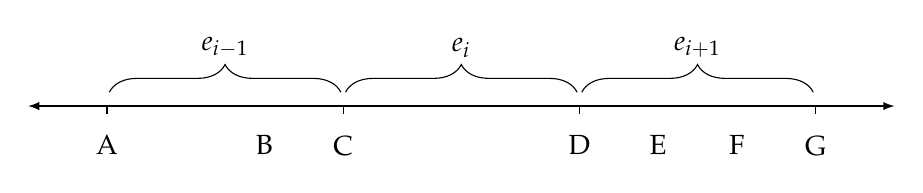
\begin{tikzpicture}
% axis
\draw[latex-latex] (0,0) -- (11,0) ;

% epoch braces
\draw [decorate,decoration={brace,amplitude=10pt} ,yshift=5pt] (1.03,0) -- (3.97,0)
  node [midway, above, yshift=9pt]{$e_{i-1}$};
\draw [decorate,decoration={brace,amplitude=10pt} ,yshift=5pt] (4.03,0) -- (6.97,0)
  node [midway, above, yshift=9pt]{$e_{i}$};
\draw [decorate,decoration={brace,amplitude=10pt} ,yshift=5pt] (7.03,0) -- (9.97,0)
  node [midway, above, yshift=9pt]{$e_{i+1}$};

% epoch boundaries
\foreach \x in  {1,4,7,10}
  \draw[shift={(\x,0)}] (0pt,0pt) -- (0pt,-3pt);

\node at (1,-0.5) {A};
\node at (3,-0.5) {B};
\node at (4,-0.5) {C};
\node at (7,-0.5) {D};
\node at (8,-0.5) {E};
\node at (9,-0.5) {F};
\node at (10,-0.5) {G};

\end{tikzpicture}

We must therefore store the last three stake distributions.
The mnemonic ``mark, set, go'' will be used to keep
track of the snapshots, where the label ``mark'' refers to the most recent snapshot,
and ``go'' refers to the snapshot that is ready to be used in the reward calculation.
In the above diagram, the snapshot taken at (A) is labeled ``mark'' during epoch $e_{i-1}$,
``set'' during epoch $e_i$ and ``go'' during epoch $e_{i+1}$. At (G) the snapshot
taken at (A) is no longer needed and will be discarded.

The two main transition systems in this section are:
\begin{itemize}
  \item The transition system named $\mathsf{EPOCH}$, which is defined in
    Section~\ref{sec:total-epoch}, covers what happens at the epoch boundary,
    such as at (A), (C), (D) and (G).
  \item The transition named $\mathsf{RUPD}$, which is defined in
    Section~\ref{sec:reward-update-trans}, covers the reward calculation that
    happens between (E) and (F).
\end{itemize}


\begin{note}
  Between time D and E we are concerned with chain growth and stability.
  Therefore this duration can be stated as 2k blocks (to state it in slots requires details about
  the particular version of the Ouroboros protocol). The duration between F and G is also 2k blocks.
  Between E and F a single honest block is enough to ensure a random nonce.
\end{note}

\subsection{Example Illustration of the Reward Cycle}
\label{sec:illustration-reward-cycle}

\definecolor{epochColor}{rgb} {1.00,0.50,0.00}
\definecolor{aliceColor}{rgb} {0.65,0.00,0.00}
\definecolor{bobColor}{rgb} {0.00,0.50,0.00}
\definecolor{bob2Color}{rgb} {0.00,0.95,0.00}
\definecolor{snapshot1}{rgb} {0.00,0.00,0.90}
\definecolor{snapshot2}{rgb} {0.00,0.60,0.90}

\begin{tikzpicture}

  % Axis
  \draw [thick] (-0.2,0) -- (13,0);
  \draw (0,-.2) -- (0, .2);
  \draw (3,-.2) -- (3, .2);
  \draw (6,-.2) -- (6, .2);
  \draw (9,-.2) -- (9, .2);
  \draw (12,-.2) -- (12, .2);
  \node[align=center, below, color=epochColor] at (1.5,0.5)
    {$e_1$};
  \node[align=center, below, color=epochColor] at (4.5,0.5)
    {$e_2$};
  \node[align=center, below, color=epochColor] at (7.5,0.5)
    {$e_3$};
  \node[align=center, below, color=epochColor] at (10.5,0.5)
    {$e_4$};

  % Alice
  % Alice's circle
  \draw [aliceColor, fill] (0,3) circle [radius=0.5];
  \node [white] at (0,3) {Alice};
  % Alice's delegation line
  \draw [->,thick, aliceColor] (0.4,2.65) to (2,0.05);
  \node [aliceColor] at (2.2,2) {delegate to Bob};

  % Bob
  % Bob's circle
  \draw [bobColor, fill] (0,-3) circle [radius=0.5];
  \node [white] at (0,-3) {Bob};
  % Bob's registration line
  \draw [->,thick, bobColor] (0.2,-2.50) to (1,-0.05);
  \node [align=left, below, bobColor] at (-0.5,-0.5) {initial pool \\ registration};
  % Bob's re-registration line
  \draw [->,thick, bob2Color] (0.45,-2.65) to (2.90,-0.05);
  \node [bob2Color] at (2,-2.8) {re-registration};
  % Bob's cached parameter change
  \draw [->,thick, bob2Color] (2.9,-0.2) to [out=280, in=180] (3,-2)
     to [out=0, in=290] (3.1,-0.2);

  % Alice time to re-delegate
  \draw [decorate, decoration = {brace, mirror, amplitude=10pt}, aliceColor, thick]
    (3.2,-0.2) to (5.9,-0.2);
  \node [align=center, below, aliceColor] at (5.1,-0.5)
    {Alice's opportunity \\ to re-delegate \\ before Bob's new \\ parameters};

  % Bob's blocks
  % epoch e3
  \draw [fill=bobColor,bobColor] (6.3,-.1) rectangle (6.5,-.3);
  \draw [fill=bobColor,bobColor] (6.7,-.1) rectangle (6.9,-.3);
  \draw [fill=bobColor,bobColor] (7.4,-.1) rectangle (7.6,-.3);
  \draw [fill=bobColor,bobColor] (8.4,-.1) rectangle (8.6,-.3);
  \draw [decorate, decoration = {brace, mirror, amplitude=10pt}, bobColor, thick]
    (6.2, -0.4) to (8.9,-0.4);
  \draw [->,thick, bobColor] (7.6, -0.8) to [out=315,in=200] (8.4, -1.2)
     to [] (9.6, -0.9);

  % epoch e4
  \draw [fill=bob2Color,bob2Color] (9.9,-.1) rectangle (10.1,-.3);
  \draw [fill=bob2Color,bob2Color] (10.4,-.1) rectangle (10.6,-.3);
  \draw [fill=bob2Color,bob2Color] (10.8,-.1) rectangle (11.0,-.3);
  \draw [decorate, decoration = {brace, mirror, amplitude=10pt}, bob2Color, thick]
    (9.7, -0.4) to (11.2,-0.4);
  \draw [->,thick, bob2Color] (10.6, -0.8) to [out=315,in=200] (11.4, -1.2)
     to [] (12.6, -0.9);

  % Snapshots
  \draw [->,thick, snapshot1] (3,0.3) to [out=90,in=150] (9,0.5)
     to [out=330,in=180] (10,-1) to [out=0,in=-135] (12,0) ;
   \node [snapshot1] at (2.7,1.2) {mark};
   \node [snapshot1] at (6,1.9) {set};
   \node [snapshot1] at (9,0.9) {go};

  \draw [->,thick, snapshot2] (6,0.3) to [out=90,in=150] (12,0.5)
     to [out=330,in=180] (13,-1);
   \node [snapshot2] at (5.7,1.2) {mark};
   \node [snapshot2] at (9,1.9) {set};
   \node [snapshot2] at (12,0.9) {go};
\end{tikzpicture}

Bob registers his stake pool in epoch $e_1$.
Alice delegates to Bob's stake pool in epoch $e_1$.
Just before the end of epoch $e_1$, Bob submits a stake pool re-registration,
changing his pool parameters. The change in parameters is not immediate,
as shown by the curved arrow around the epoch boundary.

A snapshot is taken on the $e_1$/$e_2$ boundary. It is labeled ``mark'' initially.
This snapshot includes Alice's delegation to Bob's pool, and Bob's pool parameters
and listed in the initial pool registration certificate.

If Alice changes her delegation choice any time during epoch $e_2$,
she will never be effected by Bob's change of parameters.

A new snapshot is taken on the $e_2$/$e_3$ boundary.
The previous (darker blue) snapshot is now labeled ``set'', and the new one labeled ``mark''.
The ``set'' snapshot is used for leader election in epoch $e_3$.

On the $e_3$/$e_4$ boundary, the darker blue snapshot is labeled ``go'' and
the lighter blue snapshot is labeled ``set''.
Bob's stake pool performance during epoch $e_3$ (he produced 4 blocks)
will be used with the darker blue snapshot for the rewards which will
be handed out at the beginning of epoch $e_5$.

\subsection{Helper Functions and Accounting Fields}
\label{sec:stake-dist-helpers}

Figure~\ref{fig:funcs:epoch-helper-rewards} defines four helper functions needed
throughout the rest of the section.

\begin{itemize}
  \item The function $\fun{obligation}$ calculates the the minimal amount of coin needed to
    pay out all deposit refunds.
  \item The function $\fun{poolStake}$ filters the stake distribution to one stake pool.
\end{itemize}


%%
%% Figure - Helper Functions for Epoch Rules
%%
\begin{figure}[htb]
  \emph{Total possible refunds}
  \begin{align*}
    & \fun{obligation} \in \PParams \to (\StakeCredential \mapsto \Coin)
    \to (\KeyHash_{pool}\mapsto\PoolParam) \to \Coin \\
    & \obligation{pp}{rewards}{poolParams} = \\
    & ~~~~~
    (\fun{keyDeposit}~\var{pp}) \cdot|\var{rewards}| +
    (\fun{poolDeposit}~\var{pp}) \cdot|\var{poolParams}| \\
  \end{align*}
  %
  \emph{Filter Stake to one Pool}
  \begin{align*}
      & \fun{poolStake} \in \KeyHash_{pool} \to (\KeyHash_{stake} \mapsto \KeyHash_{pool})
        \to \Stake \to \Stake \\
      & \poolStake{hk}{delegs}{stake} =
        \dom{(\var{delegs}\restrictrange\{hk\})\restrictdom\var{stake}}
  \end{align*}

  \caption{Helper Functions used in Rewards and Epoch Boundary}
  \label{fig:funcs:epoch-helper-rewards}
\end{figure}


The Figure~\ref{fig:defs:accounting} lists the accounting fields, denoted by $\Acnt$,
which will be used throughout this section. It consists of:
\begin{itemize}
  \item The value $\var{treasury}$ tracks the amount of coin currently stored in the treasury.
    Initially there will be no way to remove these funds.
  \item The value $\var{reserves}$ tracks the amount of coin currently stored in the reserves.
    This pot is used to pay rewards.
\end{itemize}
More will be said about the general accounting system in Section~\ref{sec:reward-calc}.

%%
%% Figure - Accounting fields
%%
\begin{figure}[htb]
  \emph{Accounting Fields}
  \begin{equation*}
    \Acnt =
    \left(
      \begin{array}{r@{~\in~}ll}
        \var{treasury} & \Coin & \text{treasury pot}\\
        \var{reserves} & \Coin & \text{reserve pot}\\
      \end{array}
    \right)
  \end{equation*}
  %
  \caption{Accounting fields}
  \label{fig:defs:accounting}
\end{figure}


\subsection{Stake Distribution Calculation}
\label{sec:stake-dist-calc}

This section defines the stake distribution calculations.
Figure~\ref{fig:epoch-defs} introduces three new derived types:
\begin{itemize}
  \item $\type{BlocksMade}$ represents the number of blocks each stake pool produced
    during an epoch.
  \item $\type{Stake}$ represents the amount of stake (in $\type{Coin}$) controlled by each
    stake pool.
\end{itemize}

%%
%% Figure - Epoch Abstract Types
%%
\begin{figure}[htb]
  \emph{Derived types}
  %
  \begin{equation*}
    \begin{array}{r@{~\in~}l@{\qquad=\qquad}lr}
      \var{blocks}
      & \BlocksMade
      & \KeyHash_{pool} \mapsto \N
      & \text{blocks made by stake pools} \\
      \var{stake}
      & \Stake
      & \Credential \mapsto \Coin
      & \text{stake} \\
    \end{array}
  \end{equation*}
  \caption{Epoch definitions}
  \label{fig:epoch-defs}
\end{figure}

The stake distribution calculation is given in Figure~\ref{fig:functions:stake-distribution}.

\begin{itemize}
\item $\fun{aggregate_{+}}$ takes a relation on $A\times B$, where $B$ is any
  monoid $(B,+,e)$ and returns a map from each $a\in A$ to the ``sum'' (using
  the monoidal $+$ operation) of all $b\in B$ such that $(a, b)\in A\times B$.
\item $\fun{stakeDistr}$ uses the $\fun{aggregate_{+}}$ function and several relations to
    compute the stake distribution, mapping each hashkey to the total coin under its control.
    Keys that are not both registered and delegated are filtered out.
    The relation passed to $\fun{aggregate_{+}}$ is made up of:
    \begin{itemize}
      \item $\fun{stakeCred_b}^{-1}$, relating credentials to (base) addresses
      \item $\left(\fun{addrPtr}\circ\var{ptr}\right)^{-1}$, relating credentials to (pointer)
        addresses
      \item $\range{utxo}$, relating addresses to coins
      \item $\fun{stakeCred_r}^{-1}\circ\var{rewards}$, relating (reward) addresses to coins
    \end{itemize}
    The notation for relations is explained in Section~\ref{sec:notation-shelley}.
\end{itemize}

%%
%% Figure Functions for Stake Distribution
%%
\begin{figure}[htb]
  \emph{Aggregation (for a monoid B)}
  %
  \begin{align*}
      & \fun{aggregate_{+}} \in \powerset{(A \times B)} \to (A\mapsto B) \\
      & \fun{aggregate_{+}}~\var{R} = \left\{a\mapsto \sum_{(a,b)\in\var{R}}b
          ~\mid~a\in\dom\var{R}\right\} \\
  \end{align*}
  %
  \emph{Stake Distribution (using functions and maps as relations)}
  %
  \begin{align*}
      & \fun{stakeDistr} \in \UTxO \to \DState \to \PState \to \Snapshot \\
      & \fun{stakeDistr}~{utxo}~{dstate}~{pstate} = \\
      & ~~~~ \big((\dom{\var{activeDelegs}})
      \restrictdom\left(\fun{aggregate_{+}}~\var{stakeRelation}\right),
    ~\var{delegations},~\var{poolParams}\big)\\
      & \where \\
      & ~~~~ (~\var{rewards},~\var{delegations},~\var{ptrs},~\wcard,~\wcard,~\wcard)
        = \var{dstate} \\
      & ~~~~ (~\var{poolParams},~\wcard,~\wcard) = \var{pstate} \\
      & ~~~~ \var{stakeRelation} = \left(
        \left(\fun{stakeCred_b}^{-1}\cup\left(\fun{addrPtr}\circ\var{ptr}\right)^{-1}\right)
        \circ\left(\range{\var{utxo}}\right)
        \right)
        \cup \var{rewards} \\
      & ~~~~ \var{activeDelegs} =
               (\dom{rewards}) \restrictdom \var{delegations} \restrictrange (\dom{poolParams}) \\
  \end{align*}

  \caption{Stake Distribution Function}
  \label{fig:functions:stake-distribution}
\end{figure}

\clearpage

\subsection{Snapshot Transition}
\label{sec:snapshots}

The state transition types for stake distribution snapshots are given in
Figure~\ref{fig:ts-types:snapshot}.
Each snapshot consists of:
\begin{itemize}
  \item $\var{stake}$, a stake distribution, which is defined in
    Figure~\ref{fig:epoch-defs} as a mapping of credentials to coin.
  \item $\var{delegations}$, a delegation map, mapping credentials to stake pools.
  \item $\var{poolParameters}$, storing the pool parameters of each stake pool.
\end{itemize}

The type $\type{\Snapshots}$ contains the
information needing to be saved on the epoch boundary:
\begin{itemize}
  \item $\var{pstake_{mark}}$, $\var{pstake_{set}}$ and $\var{pstake_{go}}$ are the three
    snapshots as explained in Section~\ref{sec:reward-overview}.
  \item $\var{feeSS}$ stores the fees which are added to the reward pot during
    the next reward update calculation, which is then subtracted from the fee pot
    on the epoch boundary.
\end{itemize}

%%
%% Figure - Snapshots Defs
%%
\begin{figure}[htb]
  \emph{Snapshots}
  \begin{equation*}
    \Snapshot =
    \left(
      \begin{array}{r@{~\in~}ll}
        \var{stake} & \Stake & \text{stake distribution}\\
        \var{delegations} & \Credential\mapsto\KeyHash_{pool}
                          & \text{stake delegations}\\
        \var{poolParameters} & \KeyHash_{pool} \mapsto \PoolParam & \text{pool parameters }\\
      \end{array}
    \right)
  \end{equation*}

  \begin{equation*}
    \Snapshots =
    \left(
      \begin{array}{r@{~\in~}ll}
        \var{pstake_{mark}} & \Snapshot & \text{newest stake}\\
        \var{pstake_{set}}  & \Snapshot & \text{middle stake}\\
        \var{pstake_{go}}   & \Snapshot & \text{oldest stake}\\
        \var{feeSS} & \Coin & \text{fee snapshot}\\
      \end{array}
    \right)
  \end{equation*}
  %
  \emph{Snapshot transitions}
  \begin{equation*}
    \_ \vdash
    \var{\_} \trans{snap}{} \var{\_}
    \subseteq \powerset (\LState \times \Snapshots \times \Snapshots)
  \end{equation*}
  %
  \caption{Snapshot transition-system types}
  \label{fig:ts-types:snapshot}
\end{figure}

The snapshot transition rule is given in Figure~\ref{fig:rules:snapshot}.
This transition has no preconditions and results in the following state change:

\begin{itemize}
  \item The oldest snapshot is replaced with the penultimate one.
  \item The penultimate snapshot is replaced with the newest one.
  \item The newest snapshot is replaced with one just calculated.
  \item The current fees pot is stored in $\var{feeSS}$. Note that this value will not
    change during the epoch, unlike the $\var{fees}$ value in the UTxO state.
\end{itemize}

%%
%% Figure - Snapshot Rule
%%
\begin{figure}[htb]
  \begin{equation}\label{eq:snapshot}
    \inference[Snapshot]
    {
      {
      \begin{array}{r@{~\leteq~}l}
        ((\var{utxo},~\wcard,\var{fees},~\wcard),~(\var{dstate},~\var{pstate})) & \var{lstate} \\
        \var{stake} & \stakeDistr{utxo}{dstate}{pstate} \\
      \end{array}
      }
    }
    {
      \begin{array}{r}
        \var{lstate} \\
      \end{array}
      \vdash
      \left(
        \begin{array}{r}
          \var{pstake_{mark}}\\
          \var{pstake_{set}}\\
          \var{pstake_{go}}\\
          \var{feeSS} \\
        \end{array}
      \right)
      \trans{snap}{}
      \left(
        \begin{array}{r}
          \varUpdate{\var{stake}} \\
          \varUpdate{\var{pstake_{mark}}} \\
          \varUpdate{\var{pstake_{set}}} \\
          \varUpdate{\var{fees}} \\
        \end{array}
      \right)
    }
  \end{equation}
  \caption{Snapshot Inference Rule}
  \label{fig:rules:snapshot}
\end{figure}

\clearpage

\subsection{Pool Reaping Transition}
\label{sec:pool-reap}

Figure~\ref{fig:ts-types:pool-reap} defines the types for the pool reap transition,
which is responsible for removing pools slated for retirement in the given epoch.

%%
%% Figure - Pool Reap Defs
%%
\begin{figure}[htb]
  \emph{Pool Reap State}
  \begin{equation*}
    \PlReapState =
    \left(
      \begin{array}{r@{~\in~}ll}
        \var{utxoSt} & \UTxOState & \text{utxo state}\\
        \var{acnt} & \Acnt & \text{accounting}\\
        \var{dstate} & \DState & \text{delegation state}\\
        \var{pstate} & \PState & \text{pool state}\\
      \end{array}
    \right)
  \end{equation*}
  %
  \emph{Pool Reap transitions}
  \begin{equation*}
    \_ \vdash \_ \trans{poolreap}{\_} \_ \in
    \powerset (\PParams \times \PlReapState \times \Epoch \times \PlReapState)
  \end{equation*}
  %
  \caption{Pool Reap Transition}
  \label{fig:ts-types:pool-reap}
\end{figure}


The pool-reap transition rule is given in Figure~\ref{fig:rules:pool-reap}.
This transition has no preconditions and results in the following state change:

\begin{itemize}
  \item For each retiring pool, the refund for the pool registration deposit is added to the
    pool's registered reward account, provided the reward account is still registered.
  \item The sum of all the refunds attached to unregistered reward accounts are added to the
    treasury.
  \item The deposit pool is reduced by the amount of claimed and unclaimed refunds.
  \item Any delegation to a retiring pool is removed.
  \item Each retiring pool is removed from all four maps in the pool state.
\end{itemize}

%%
%% Figure - Pool Reap Rule
%%
\begin{figure}[htb]
  \begin{equation}\label{eq:pool-reap}
    \inference[Pool-Reap]
    {
      {
      \begin{array}{r@{~\leteq~}l}
        \var{retired} & \dom{(\var{retiring}^{-1}~\var{e})} \\
        \var{pr} & \left\{
                   \var{hk}\mapsto(\fun{poolDeposit}~\var{pp})
                     \mid
                     \var{hk}\in\var{retired}
                   \right\}\\
        \var{rewardAcnts}
                 & \{\var{hk}\mapsto \fun{poolRAcnt}~\var{pool} \mid
                   \var{hk}\mapsto\var{pool} \in \var{retired}\restrictdom\var{poolParams} \} \\
        \var{rewardAcnts'} & \left\{
                               \sum\limits_{\wcard\mapsto c\in\var{pr}\circ\var{rewardAcnts}^{-1}(a)} c
                               \mathrel{\Bigg|}
			       a\in\range{rewardAcnts}
                             \right\} \\
        \var{refunds} & \dom{rewards}\restrictdom\var{rewardAcnts'} \\
        \var{mRefunds} & \dom{rewards}\subtractdom\var{rewardAcnts'} \\
        \var{refunded} & \sum\limits_{\wcard\mapsto c\in\var{refunds}} c \\
        \var{unclaimed} & \sum\limits_{\wcard\mapsto c\in\var{mRefunds}} c \\
      \end{array}
      }
    }
    {
      \var{pp}
      \vdash
      \left(
        \begin{array}{r}
          \var{utxo} \\
          \var{deposited} \\
          \var{fees} \\
          \var{ppup} \\
          ~ \\
          \var{treasury} \\
          \var{reserves} \\
          ~ \\
          \var{rewards} \\
          \var{delegations} \\
          \var{ptrs} \\
          \var{genDelegs} \\
          \var{fGenDelegs} \\
          \var{i_{rwd}} \\
          ~ \\
          \var{poolParams} \\
          \var{fPoolParams} \\
          \var{retiring} \\
        \end{array}
      \right)
      \trans{poolreap}{e}
      \left(
        \begin{array}{rcl}
          \var{utxo} \\
          \varUpdate{\var{deposited}}
          & \varUpdate{-}
          & \varUpdate{(\var{unclaimed} + \var{refunded})} \\
          \var{fees} \\
          \var{ppup} \\
          ~ \\
          \varUpdate{\var{treasury}} & \varUpdate{+} & \varUpdate{\var{unclaimed}} \\
          \var{reserves} \\
          ~ \\
          \varUpdate{\var{rewards}} & \varUpdate{\unionoverridePlus} & \varUpdate{\var{refunds}} \\
          \varUpdate{\var{delegations}} & \varUpdate{\subtractrange} & \varUpdate{\var{retired}} \\
          \var{ptrs} \\
          \var{genDelegs} \\
          \var{fGenDelegs} \\
          \var{i_{rwd}}\\
          ~ \\
          \varUpdate{\var{retired}} & \varUpdate{\subtractdom} & \varUpdate{\var{poolParams}} \\
          \varUpdate{\var{retired}} & \varUpdate{\subtractdom} & \varUpdate{\var{fPoolParams}} \\
          \varUpdate{\var{retired}} & \varUpdate{\subtractdom} & \varUpdate{\var{retiring}} \\
        \end{array}
      \right)
    }
  \end{equation}
  \caption{Pool Reap Inference Rule}
  \label{fig:rules:pool-reap}
\end{figure}

\clearpage

\subsection{Protocol Parameters Update Transition}
\label{sec:pparam-update}

Finally, reaching the epoch boundary may trigger a change in the protocol parameters.
The protocol parameters environment consists of the delegation and pool states,
and the signal is an optional new collection of protocol parameters
The state change is a change of the $\UTxOState$, the $\Acnt$ states and the current $\PParams$.
The type of this state transition is given in Figure~\ref{fig:ts-types:new-proto-param}.

%%
%% Figure - New Proto Param Defs
%%
\begin{figure}[htb]
  \emph{New Proto Param environment}
  \begin{equation*}
    \NewPParamEnv =
    \left(
      \begin{array}{r@{~\in~}ll}
        \var{dstate} & \DState & \text{delegation state}\\
        \var{pstate} & \PState & \text{pool state}\\
      \end{array}
    \right)
  \end{equation*}
  %
  \emph{New Proto Param States}
  \begin{equation*}
    \NewPParamState =
    \left(
      \begin{array}{r@{~\in~}ll}
        \var{utxoSt} & \UTxOState & \text{utxo state}\\
        \var{acnt} & \Acnt & \text{accounting}\\
        \var{pp} & \PParams & \text{current protocol parameters}\\
      \end{array}
    \right)
  \end{equation*}
  %
  \emph{New Proto Param transitions}
  \begin{equation*}
    \_ \vdash
    \var{\_} \trans{newpp}{\_} \var{\_}
    \subseteq \powerset (\NewPParamEnv \times \NewPParamState \times \PParams^? \times \NewPParamState)
  \end{equation*}
  %
  \caption{New Proto Param transition-system types}
  \label{fig:ts-types:new-proto-param}
  %
  \emph{Helper Functions}
  \begin{align*}
      & \fun{updatePpup} \in \UTxOState \to \PParams \to \UTxOState\\
      & \fun{updatePpup}~\var{utxoSt}~\var{pp} =
      \begin{cases}
        (\var{utxo},\var{deposited},\var{fees},(\var{fpup},~\emptyset))
        &
        \var{canFollow}
        \\
        (\var{utxo},\var{deposited},\var{fees},(\emptyset,~\emptyset))
        &
        \text{otherwise} \\
      \end{cases}\\
      & ~~~\where \\
      & ~~~~~~~\var{canFollow} =
        \forall\var{ps}\in\range{pup},~
        \var{pv}\mapsto\var{v}\in\var{ps}\implies\fun{pvCanFollow}~(\fun{pv}~\var{pp})~\var{v}
        \\
      & ~~~~~~~(\var{utxo},\var{deposited},\var{fees},(\var{pup},~\var{fpup})) = \var{utxoSt} \\
  \end{align*}
\end{figure}


Figure~\ref{fig:rules:new-proto-param} defines the new protocol parameter transition.
The transition has two rules, depending on whether or not the new protocol parameters
meet some requirements.
In particular, we require that the new parameters would not incur a debt of the system that
can not be covered by the reserves, and that the max block size is greater than the sum of the
max transaction size and the max header size.
If the requirements are met, the new protocol parameters are accepted, the proposal is reset,
and the reserves are adjusted to account for changes in the deposits.
Otherwise, the only change is that the proposal is reset.

The $\mathsf{NEWPP}$ rule also cleans up the protocol parameter update proposals,
by calling $\fun{updatePpup}$ on the UTxO state.
The $\fun{updatePpup}$ sets the protocol parameter updates to the future protocol
parameter updates provided the protocol versions all can follow from the
version given in the protocol parameters, or the emptyset otherwise.
In any case, the future protocol parameters update proposals are set to the empty set.
If new protocol parameters are being adopted, then these is the value given to
$\fun{updatePpup}$, otherwise the old parameters are given.

Regarding adjusting the reserves for changes in the deposits, one of three things happens:

\begin{itemize}
  \item If the new protocol parameters mean that \textbf{fewer} funds are required in the
    deposit pot to cover all possible refunds, then the excess is moved to the reserves.

  \item If the new protocol parameters mean that \textbf{more} funds are required in the
    deposit pot to cover all possible refunds and the difference is \textbf{less} than
    the reserve pot, then funds are moved from the reserve pot to cover the difference.

  \item If the new protocol parameters mean that \textbf{more} funds are required in the
    deposit pot to cover all possible refunds and the difference is \textbf{more} than
    the reserve pot, then Rule~\ref{eq:new-pc-denied} meets the precondition and the
    only change of state is that the update proposals are reset.
\end{itemize}

Note that here, unlike most of the inference rules in this document,
the $\var{utxoSt'}$ and the $\var{acnt'}$ do not come from valid UTxO or
accounts transitions in the antecedent. We simply define the consequent
transition using these directly (instead of listing all the fields in both
states in the consequent transition). It is done this way here
for ease of reading.

%%
%% Figure - New Proto Param Rule
%%
\begin{figure}[htb]
  \begin{equation}\label{eq:new-pc-accepted}
    \hspace{-0.3cm}
    \inference[New-Proto-Param-Accept]
    {
      \var{pp_{new}}\neq\Nothing \\~\\
      {\begin{array}{rcl}
         (\var{utxo},~\var{deposited},~\var{fees},~\var{ppup}) & \leteq & \var{utxoSt} \\
         \var{(\var{rewards},~\wcard,~\wcard,~\wcard,~\wcard,~\var{i_{rwd}})} &
         \leteq & \var{dstate}\\
         \var{(\var{poolParams},~\wcard,~\wcard)} & \leteq & \var{pstate}\\
         \var{oblg_{cur}} & \leteq & \obligation{pp}{rewards}{poolParams} \\
         \var{oblg_{new}} & \leteq & \obligation{pp_{new}}{rewards}{poolParams} \\
         \var{diff} & \leteq & \var{oblg_{cur}} - \var{oblg_{new}}\\
      \end{array}}
      \\~\\~\\
      \var{oblg_{cur}} = \var{deposited} \\
      \var{reserves} + \var{diff} \geq \sum\limits_{\wcard\mapsto\var{val}\in\var{i_{rwd}}} val \\
      \fun{maxTxSize}~\var{pp_{new}} + \fun{maxHeaderSize}~\var{pp_{new}} <
        \fun{maxBlockSize}~\var{pp_{new}}
      \\~\\
        \var{utxoSt'} \leteq
        \left(\var{utxo},~\varUpdate{oblg_{new}},~\var{fees},~\var{ppup}\right)
      \\
      \var{utxoSt''} \leteq \fun{updatePpup}~\var{utxoSt'}~\var{pp_{new}}
      \\~\\
      (\var{treasury},~\var{reserves})\leteq \var{acnt} \\
      \var{acnt'} \leteq (\var{treasury},~\varUpdate{reserves + diff}) \\
    }
    {
      \begin{array}{l}
        \var{dstate}\\
        \var{pstate}\\
      \end{array}
      \vdash
      \left(
        \begin{array}{r}
          \var{utxoSt} \\
          \var{acnt} \\
          \var{pp}
        \end{array}
      \right)
      \trans{newpp}{\var{pp_{new}}}
      \left(
        \begin{array}{rcl}
          \varUpdate{utxoSt''}\\
          \varUpdate{acnt'} \\
          \varUpdate{\var{pp_{new}}} \\
        \end{array}
      \right)
    }
  \end{equation}

  \nextdef

  \begin{equation}\label{eq:new-pc-denied}
    \inference[New-Proto-Param-Denied]
    {
      \left({\begin{array}{c}
            \var{pp_{new}}=\Nothing \\
        \lor \\
        \var{reserves} + \var{diff} < \sum\limits_{\wcard\mapsto\var{val}\in\var{i_{rwd}}} val\\
        \lor \\
        \fun{maxTxSize}~\var{pp_{new}} + \fun{maxHeaderSize}~\var{pp_{new}} \geq
          \fun{maxBlockSize}~\var{pp_{new}}
      \end{array}}\right)
      \\~\\~\\
      {\begin{array}{rcl}
          \var{(\var{rewards},~\wcard,~\wcard,~\wcard,~\wcard,~\var{i_{rwd}})} &
          \leteq & \var{dstate}\\
         \var{(\var{poolParams},~\wcard,~\wcard)} & \leteq & \var{pstate}\\
          \var{oblg_{cur}} & \leteq & \obligation{pp}{rewards}{poolParams} \\
          \var{oblg_{new}} & \leteq & \obligation{pp_{new}}{rewards}{poolParams} \\
         \var{diff} & \leteq & \var{oblg_{cur}} - \var{oblg_{new}}
      \end{array}}
      \\~\\~\\
      \var{utxoSt'} \leteq \fun{updatePpup}~\var{utxoSt}~\var{pp} \\
    }
    {
      \begin{array}{l}
        \var{dstate}\\
        \var{pstate}\\
      \end{array}
      \vdash
      \left(
        \begin{array}{r}
          \var{utxoSt} \\
          \var{acnt} \\
          \var{pp}
        \end{array}
      \right)
      \trans{newpp}{\var{pp_{new}}}
      \left(
        \begin{array}{rcl}
          \varUpdate{utxoSt'}\\
          \var{acnt} \\
          \var{pp}
        \end{array}
      \right)
    }
  \end{equation}
  \caption{New Proto Param Inference Rule}
  \label{fig:rules:new-proto-param}
\end{figure}

\clearpage

\subsection{Complete Epoch Boundary Transition}
\label{sec:total-epoch}

Finally, it is possible to define the complete epoch boundary transition type,
which is defined in Figure~\ref{fig:ts-types:epoch}.
The transition has no evironment.
The state is made up of the the accounting state, the snapshots, the ledger state and the
protocol parameters.
The transition uses a helper function $\fun{votedValue}$ which returns
the consensus value of update proposals in the event that consensus is met.
\textbf{Note that} $\fun{votedValue}$
\textbf{is only well-defined if } $\var{quorum}$
\textbf{is greater than half the number of core nodes, i.e.}
$\Quorum > |\var{genDelegs}|/2$ \textbf{.}

%%
%% Figure - Epoch Defs
%%
\begin{figure}[htb]
  \emph{Epoch States}
  \begin{equation*}
    \EpochState =
    \left(
      \begin{array}{r@{~\in~}ll}
        \var{acnt} & \Acnt & \text{accounting}\\
        \var{ss} & \Snapshots & \text{snapshots}\\
        \var{ls} & \LState & \text{ledger state}\\
        \var{prevPp} & \PParams & \text{previous protocol parameters}\\
        \var{pp} & \PParams & \text{protocol parameters}\\
      \end{array}
    \right)
  \end{equation*}
  %
  \emph{Epoch transitions}
  \begin{equation*}
    \vdash
    \var{\_} \trans{epoch}{\_} \var{\_}
    \subseteq \powerset (\EpochState \times \Epoch \times \EpochState)
  \end{equation*}
  %
  \emph{Accessor Functions}
  \begin{equation*}
    \begin{array}{r@{~\in~}lr}
      \fun{getIR} & \EpochState \to (\StakeCredential \mapsto \Coin)
                  & \text{get instantaneous rewards} \\
    \end{array}
  \end{equation*}
  %
  \emph{Helper Functions}
  \begin{align*}
      & \fun{votedValue} \in (\KeyHashGen\mapsto\PParamsUpdate) \to \PParams \to \N \to \PParamsUpdate^?\\
      & \fun{votedValue}~\var{pup}~\var{pp}~\var{quorum} =
      \begin{cases}
        \var{pp}\unionoverrideRight\var{p}
          & \exists! p\in\range{pup}~(|pup\restrictrange p|\geq \var{quorum}) \\
        \Nothing & \text{otherwise} \\
      \end{cases}
  \end{align*}
  %
  \caption{Epoch transition-system types}
  \label{fig:ts-types:epoch}
\end{figure}


The epoch transition rule calls $\mathsf{SNAP}$, $\mathsf{POOLREAP}$ and $\mathsf{NEWPP}$
in sequence. It also stores the previous protocol parameters in $\var{prevPp}$.
The previous protocol parameters will be used for the reward calculation in the upcoming epoch,
note that they correspond to the epoch for which the rewards are being calculated.
Additionally, this transition also adopts the pool parameters $\var{fPoolParams}$
corresponding to the pool re-registration certificates which we submitted late in the ending epoch.
The ordering of these rules is important.
The stake pools which will be updated by $\var{fPoolParams}$ or
reaped during the $\mathsf{POOLREAP}$ transition must still be a
part of the new snapshot, and so $\mathsf{SNAP}$ must occur before these two actions.
Moreover, $\mathsf{SNAP}$ sets the deposit pot equal to current obligation,
which is a property that is preserved by $\mathsf{POOLREAP}$ and which
is necessary for the preservation of Ada property in the $ \mathsf{NEWPP}$ transition.

%%
%% Figure - Epoch Rule
%%
\begin{figure}[htb]
  \begin{equation}\label{eq:epoch}
    \inference[Epoch]
    {
      {
        \begin{array}{r}
          \var{lstate} \\
        \end{array}
      }
      \vdash
      { \var{ss} }
      \trans{\hyperref[fig:rules:snapshot]{snap}}{}
      { \var{ss'} }
      \\~\\
      (\var{utxoSt},~(\var{dstate},~\var{pstate}))\leteq\var{ls} \\
      (\var{poolParams},~\var{fPoolParams},~\var{retiring})\leteq\var{pstate}
      \\
      \var{pstate'}\leteq(\var{poolParams}\unionoverrideRight\var{fPoolParams},
      ~\emptyset,~\var{retiring})
      \\~\\~\\
      \var{pp}
      \vdash
      \left(
        {
          \begin{array}{r}
            \var{utxoSt} \\
            \var{acnt} \\
            \var{dstate} \\
            \var{pstate'} \\
          \end{array}
        }
      \right)
      \trans{\hyperref[fig:rules:pool-reap]{poolreap}}{e}
      \left(
      {
        \begin{array}{rcl}
            \var{utxoSt'} \\
            \var{acnt'} \\
            \var{dstate'} \\
            \var{pstate''} \\
        \end{array}
      }
      \right)
      \\~\\~\\
      \var{(\wcard,~\wcard,~\wcard,~(\var{pup},\wcard))}\leteq\var{utxoSt'}\\
      \var{pp_{new}}\leteq\fun{votedValue}~\var{pup}~\var{pp}~\Quorum\\
      {
        \begin{array}{r}
          \var{dstate'}\\
          \var{pstate''}\\
        \end{array}
      }
      \vdash
      \left(
        {
          \begin{array}{r}
            \var{utxoSt'} \\
            \var{acnt'} \\
            \var{pp}\\
          \end{array}
        }
      \right)
      \trans{\hyperref[fig:rules:new-proto-param]{newpp}}{\var{pp_{new}}}
      \left(
      {
        \begin{array}{rcl}
            \var{utxoSt''} \\
            \var{acnt''} \\
            \var{pp'}\\
        \end{array}
      }
      \right)
      \\~\\~\\
      \var{ls}' \leteq (\var{utxoSt}'',~(\var{dstate}',~\var{pstate}''))
    }
    {
      \vdash
      \left(
      \begin{array}{r}
        \var{acnt} \\
        \var{ss} \\
        \var{ls} \\
        \var{prevPp} \\
        \var{pp} \\
      \end{array}
      \right)
      \trans{epoch}{e}
      \left(
      \begin{array}{rcl}
        \varUpdate{\var{acnt''}} \\
        \varUpdate{\var{ss'}} \\
        \varUpdate{\var{ls'}} \\
        \varUpdate{\var{pp}} \\
        \varUpdate{\var{pp'}} \\
      \end{array}
      \right)
    }
  \end{equation}
  \caption{Epoch Inference Rule}
  \label{fig:rules:epoch}
\end{figure}

\clearpage

\subsection{Rewards Distribution Calculation}
\label{sec:reward-dist}

This section defines the reward calculation for the proof of stake leader election.
Figure~\ref{fig:functions:rewards} defines the pool reward as described in section
5.5.2 of~\cite{delegation_design}.

\begin{itemize}
  \item The function $\fun{maxPool}$ gives the maximum reward a stake pool can receive in an epoch.
    This is a fraction of the total available rewards for the epoch.
    The result depends on the pool's relative stake, the pool's pledge and the following
    protocol parameters:
    \begin{itemize}
      \item $\var{a_0}$, the leader-stake influence
      \item $n_{opt}$, the optimal number of saturated stake pools
    \end{itemize}
  \item The function $\fun{mkApparentPerformance}$ computes the apparent performance of a stake pool.
    It depends on the protocol parameter $d$, the relative stake $\sigma$, the number $n$ of blocks
    the pool added to the chain and the total number $\overline{N}$ of blocks added to the chain in
    the last epoch.

\end{itemize}

%%
%% Figure - Functions for the Reward Calculation
%%
\begin{figure}[htb]
  \emph{Maximal Reward Function, called $f(s,\sigma)$ in section 5.5.2 of~\cite{delegation_design}}
  %
  \begin{align*}
      & \fun{maxPool} \in \PParams \to \Coin \to \unitInterval \to \unitInterval \to \Coin \\
      & \fun{maxPool}~\var{pp}~\var{R}~\sigma~\var{p_r} =
          ~~~\floor*{
             \frac{R}{1 + a_0}
             \cdot
             \left(
               \sigma' + p'\cdot a_0\cdot\frac{\sigma' - p'\frac{z_0-\sigma'}{z_0}}{z_0}
             \right)} \\
      & ~~~\where \\
      & ~~~~~~~a_0 = \fun{influence}~pp \\
      & ~~~~~~~n_{opt} = \fun{nopt}~pp \\
      & ~~~~~~~z_0 = 1/n_{opt} \\
      & ~~~~~~~\sigma'=\min(\sigma,~z_0) \\
      & ~~~~~~~p'=\min(p_r,~z_0) \\
  \end{align*}

  \emph{Apparent Performance, called $\hat{p}$ in section 5.5.2 of~\cite{delegation_design}}
  %
  \begin{align*}
      & \fun{mkApparentPerformance} \in \unitInterval \to \unitInterval \to \N \to \N \to \Q \\
      & \mkApparentPerformance{d}{\sigma}{n}{\overline{N}} =
        \begin{cases}
          \frac{\beta}{\sigma} & \text{if } d < 0.8 \\
          1 & \text{otherwise}
        \end{cases} \\
      & ~~~\where \\
      & ~~~~~~~\beta = \frac{n}{\max(1, \overline{N})} \\
  \end{align*}
  \caption{Functions used in the Reward Calculation}
  \label{fig:functions:rewards}
\end{figure}

\clearpage

Figure~\ref{fig:functions:reward-splitting} gives the calculation for
splitting the pool rewards with its members, as described in 6.5.2 of \cite{delegation_design}.
The portion of rewards allocated to the pool operator and owners is different
than that of the members.

\begin{itemize}
  \item The $\fun{r_{operator}}$ function calculates the leader reward, based on the pool cost,
    margin and the proportion of the pool's total stake.  Note that this reward will go to the
    reward account specified in the pool registration certificate.
  \item The $\fun{r_{member}}$ function calculates the member reward, proportionally to their
    stake after the cost and margin are removed.
\end{itemize}

%%
%% Figure - Functions for the Reward Splitting
%%
\begin{figure}[htb]
  \emph{Pool leader reward, from section 5.5.3 of \cite{delegation_design}}
  %
  \begin{align*}
      & \fun{r_{operator}} \in \Coin \to \PoolParam \to \unitInterval \to \unitIntervalNonNull \to \Coin \\
      & \lReward{\hat{f}}{pool}{s}{\sigma} =
        \begin{cases}
        \hat{f} & \hat{f} \leq c\\
        c + \floor*{(\hat{f} - c)\cdot\left(m + (1-m)\cdot\frac{s}{\sigma}\right) }&
        \text{otherwise.}
      \end{cases} \\
      & ~~~\where \\
      & ~~~~~~~c = \fun{poolCost}~pool \\
      & ~~~~~~~m = \fun{poolMargin}~pool \\
  \end{align*}

  \emph{Pool member reward, from section 5.5.3 of \cite{delegation_design}}
  %
  \begin{align*}
    & \fun{r_{member}} \in \Coin \to \PoolParam \to \unitInterval \to \unitIntervalNonNull \to \Coin \\
    & \mReward{\hat{f}}{pool}{t}{\sigma} =
      \begin{cases}
        0 & \hat{f} \leq c\\
        \floor*{(\hat{f} - c)\cdot(1-m)\cdot\frac{t}{\sigma}} &
        \text{otherwise.}
      \end{cases} \\
    & ~~~\where \\
    & ~~~~~~~c = \fun{poolCost}~pool \\
    & ~~~~~~~m = \fun{poolMargin}~pool \\
  \end{align*}

  \caption{Functions used in the Reward Splitting}
  \label{fig:functions:reward-splitting}
\end{figure}


Finally, the full reward calculation is presented in Figure~\ref{fig:functions:reward-calc}.
The calculation is done pool-by-pool.
\begin{itemize}
\item The $\fun{rewardOnePool}$ function calculates the rewards given out to
  each member of a given pool. The pool leader is identified by the stake
  credential of the pool operator. The function returns the rewards, calculated
  as follows:
    \begin{itemize}
      \item $\var{pstake}$, the total amount of stake controlled by the stake pool.
      \item $\var{ostake}$, the total amount of stake controlled by the stake pool operator
        and owners
      \item $\sigma$, the total proportion of stake controlled by the stake pool.
      \item $\overline{N}$, the expected number of blocks the pool should have produced.
      \item $\var{pledge}$, the pool's pledge in lovelace.
      \item $p_r$, the pool's pledge, as a proportion of active stake.
      \item $\var{maxP}$, maximum rewards the pool can claim if the pledge is met,
        and zero otherwise.
      \item $\var{poolR}$, the pool's actual reward, based on its performance.
      \item $\var{mRewards}$, the member's rewards as a mapping of reward accounts to coin.
      \item $\var{lReward}$, the leader's reward as coin.
      \item $\var{potentialRewards}$, the combination of $\var{mRewards}$ and $\var{lRewards}$.
      \item $\var{rewards}$, the restriction of $\var{potentialRewards}$ to the active
        reward accounts.
    \end{itemize}
  \item The $\fun{reward}$ function applies $\fun{rewardOnePool}$ to each registered stake pool.
\end{itemize}

%%
%% Figure - The Reward Calculation
%%
\begin{figure}[htb]
  \emph{Calculation to reward a single stake pool}
  %
  \begin{align*}
    & \fun{rewardOnePool} \in \PParams \to \Coin \to \N \to \N \to \PoolParam\\
      & ~~~\to \Stake \to \Q \to \Q \to \Coin \to \powerset{\AddrRWD}
           \to (\AddrRWD \mapsto \Coin) \\
      & \fun{rewardOnePool}~\var{pp}~\var{R}~\var{n}~\var{\overline{N}}~\var{pool}~\var{stake}~{\sigma}~{\sigma_a}~\var{tot}~\var{addrs_{rew}} =
          \var{rewards}\\
      & ~~~\where \\
      & ~~~~~~~\var{ostake} = \sum_{\substack{
        hk_\mapsto c\in\var{stake}\\
        hk\in(\fun{poolOwners}~\var{pool})\\
        }} c \\
      & ~~~~~~~\var{pledge} = \fun{poolPledge}~pool \\
      & ~~~~~~~p_{r} = \var{pledge} / \var{tot} \\
      & ~~~~~~~maxP =
      \begin{cases}
        \fun{maxPool}~\var{pp}~\var{R}~\sigma~\var{p_r}&
        \var{pledge} \leq \var{ostake}\\
        0 & \text{otherwise.}
      \end{cases} \\
      & ~~~~~~~\var{appPerf} = \mkApparentPerformance{(\fun{d}~pp)}{\sigma_a}{n}{\overline{N}} \\
      & ~~~~~~~\var{poolR} = \floor{\var{appPerf}\cdot\var{maxP}} \\
      & ~~~~~~~\var{mRewards} = \\
      & ~~~~~~~~~~\left\{
                    \addrRw~hk\mapsto\mReward{poolR}{pool}{\frac{c}{tot}}{\sigma}
                    ~\Big\vert~
                    hk\mapsto c\in\var{stake},~~hk \not\in(\fun{poolOwners}~\var{pool})
                  \right\}\\
      & ~~~~~~~\var{lReward} = \lReward{poolR}{pool}{\frac{\var{ostake}}{tot}}{\sigma} \\
      & ~~~~~~~\var{potentialRewards} =
                 \var{mRewards} \cup
                 \{(\fun{poolRAcnt}~\var{pool})\mapsto\var{lReward}\} \\
      & ~~~~~~~\var{rewards} = \var{addrs_{rew}}\restrictdom{\var{potentialRewards}} \\
  \end{align*}

  \emph{Calculation to reward all stake pools}
  %
  \begin{align*}
      & \fun{reward} \in \PParams \to \BlocksMade \to \Coin\to \powerset{\AddrRWD}
      \to (\KeyHash \mapsto \PoolParam) \\
      & ~~~\to \Stake \to (\KeyHash_{stake} \mapsto \KeyHash_{pool}) \to
      \Coin \to (\AddrRWD \mapsto \Coin)\\
      & \reward{pp}{blocks}{R}{addrs_{rew}}{poolParams}{stake}{delegs}{total}
          = \var{rewards}\\
      & ~~~\where \\
      & ~~~~~~~\var{total}_a = \sum_{\_\mapsto c\in \var{stake}}c \\
      & ~~~~~~~\var{\overline{N}} = \sum_{\_\mapsto m\in blocks}m \\
      & ~~~~~~~pdata = \left\{
        hk\mapsto \left(p,~n,~\poolStake{hk}{delegs}{stake}\right)
        \mathrel{\Bigg|}
        \begin{array}{r@{\mapsto}c@{~\in~}l}
          hk & \var{p} & \var{poolParams} \\
          hk & \var{n} & \var{blocks} \\
        \end{array}
      \right\} \\
      & ~~~~~~~\var{results} = \\
      & ~~~~~~~\left\{
        hk \mapsto \fun{rewardOnePool}~
                     \var{pp}~
                     \var{R}~
                     \var{n}~
                     \var{\overline{N}}~
                     \var{p}~
                     \var{s}~
                     \frac{\sum s}{total}~
                     \frac{\sum s}{\var{total}_a}~
                     \var{total}~
                     \var{addrs_{rew}}
                 \mid
        hk\mapsto(p, n, s)\in\var{pdata} \right\} \\
      & ~~~~~~~\var{rewards} = \bigcup_{\wcard\mapsto\var{r}\in\var{results}}\var{r}
  \end{align*}
  \caption{The Reward Calculation}
  \label{fig:functions:reward-calc}
\end{figure}

\clearpage

\subsection{Reward Update Calculation}
\label{sec:reward-calc}

This section defines the calculation of a reward update.
A reward update is the information needed to account for the movement of lovelace
in the system due to paying out rewards.

Figure~\ref{fig:fund-preservation} captures the potential movement of funds in the entire system,
taking every transition system in this document into account.  Value is moved between
accounting pots, but the total amount of value in the system remains constant.
In particular, the red subgraph represents the inputs and outputs to
the ``reward pot'', a temporary variable used during the reward update calculation in
Figure~\ref{fig:functions:reward-update-creation}.
The blue arrows represent the movement of funds that pass through the ``reward pot''.


\begin{figure}[htb]
  \begin{center}
    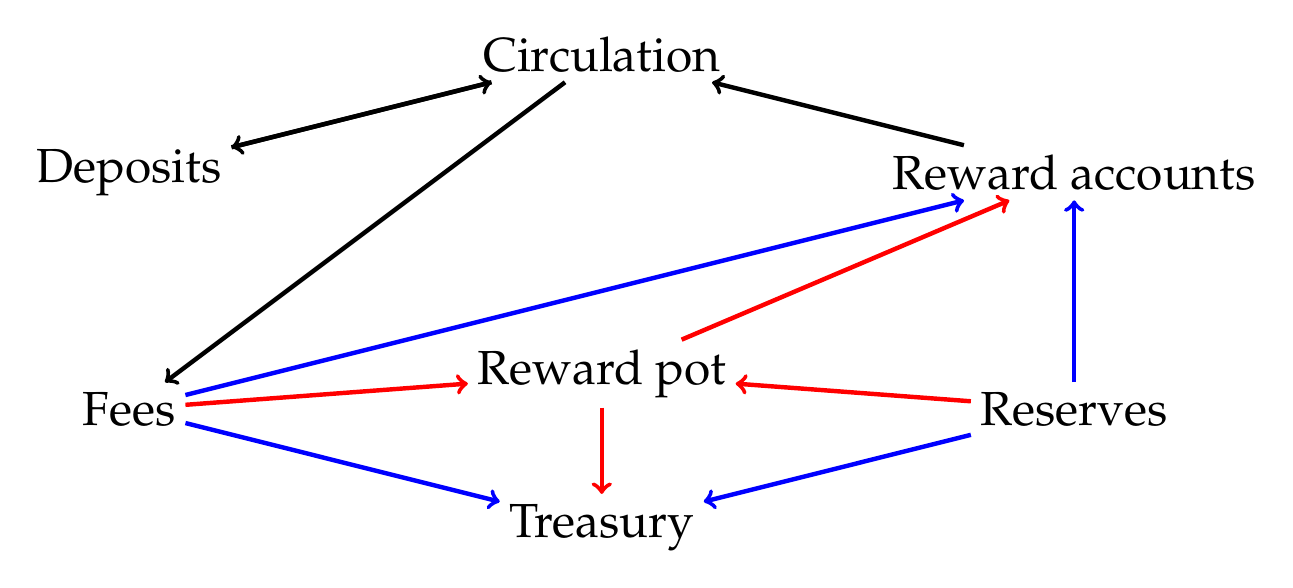
\begin{tikzpicture}
      [ x=30mm, y=30mm
      , direct/.style={black, draw}
      , implied/.style={blue, draw}
      , toTotPot/.style={red, draw}
      ]
    \node (C) at (3,2.5) {\LARGE Circulation};
    \node (R) at (5, 1) {\LARGE Reserves};
    \node (D) at (1, 2) {\LARGE Deposits};
    \node (FR) at (1,1) {\LARGE Fees};
    \node (RA) at (5, 2) {\LARGE Reward accounts};
    \node (T) at (3,0.5) {\LARGE Treasury};

    \draw[->, direct, ultra thick]
    (C) edge (D)
    (C) edge (FR)

    (D) edge (C)

    (RA) edge (C);

    \draw[->, implied, ultra thick]
    (FR) edge (T)
    (FR) edge (RA)

    (R) edge (T)
    (R) edge (RA);

    \node (TP) at (3, 1.15) {\LARGE Reward pot};

    \draw[->, toTotPot, ultra thick]
    (FR) edge (TP)
    (R) edge (TP)

    (TP) edge (RA)
    (TP) edge (T);
    \end{tikzpicture}
  \end{center}
  \caption{Preservation of Value}
  \label{fig:fund-preservation}
\end{figure}

Figure~\ref{fig:defs:reward-update} defines a reward update.
It consists of four pots:
\begin{itemize}
  \item The change to the treasury. This will be a positive value.
  \item The change to the reserves. This will be a negative value.
  \item The map of new individual rewards (to be added to the existing rewards).
  \item The change to the fee pot. This will be a negative value.
    rewards.
\end{itemize}

%%
%% Figure - Reward Update Defs
%%
\begin{figure}[htb]
  \emph{Reward Update}
  \begin{equation*}
    \RewardUpdate =
    \left(
      \begin{array}{r@{~\in~}ll}
        \Delta t & \Coin & \text{change to the treasury} \\
        \Delta r & \Coin & \text{change to the reserves} \\
        \var{rs} & \AddrRWD\mapsto\Coin & \text{new individual rewards} \\
        \Delta f & \Coin & \text{change to the fee pot} \\
      \end{array}
    \right)
  \end{equation*}
  %
  \caption{Rewards Update type}
  \label{fig:defs:reward-update}
\end{figure}

\clearpage

Figure~\ref{fig:functions:reward-update-creation} defines two functions,
$\fun{createRUpd}$ to create a reward update and $\fun{applyRUpd}$ to apply a
reward update to an instance of $\EpochState$.

The $\fun{createRUpd}$ function does the following:
\begin{itemize}
  \item Note that for all the calculations below, we use the previous protocol parameters
    $\var{prevPp}$, which corresponds to the parameters during the epoch for which we
    are creating rewards.
  \item First we calculate the change to the reserves,
    as determined by the $\rho$ protocol parameter.
  \item Next we calculate $\var{rewardPot}$, the total amount of coin available for rewards this
    epoch, as described in section 6.4 of \cite{delegation_design}. It consists of:
    \begin{itemize}
      \item The fee pot, containing the transaction fees from the epoch.
      \item The amount of monetary expansion from the reserves, calculated above.
    \end{itemize}
    Note that the fee pot is taken from the snapshot taken at the epoch boundary.
    (See~Figure\ref{fig:rules:snapshot}).
  \item Next we calculate the proportion of the reward pot that will move to the treasury,
    as determined by the $\tau$ protocol parameter. The remaining pot is called the
    $\var{R}$, just as in section 6.5 of \cite{delegation_design}.
  \item The rewards are calculated, using the oldest stake distribution snapshot (the one
    labeled ``go'').
    As given by $\fun{maxPool}$, each pool can receive a maximal amount, determined by its
    performance.  The difference between the maximal amount and the actual amount received is
    added to the amount moved to the treasury.
  \item The fee pot will be reduced by $\var{feeSS}$.
\end{itemize}

Note that fees are not explicitly removed from any account:
the fees come from transactions paying them and are accounted for whenever
transactions are processed.

The $\fun{applyRUpd}$ function does the following:
    \begin{itemize}
      \item Adjust the treasury, reserves and fee pots by the appropriate amounts.
      \item Add each individual reward to the global reward mapping.
        We must be careful, though, not to give out rewards to accounts
        that have been deregistered after the reward update was created.
        \begin{itemize}
          \item Rewards for accounts that are still registered are added to the reward mappings.
          \item The sum of the unregistered rewards are added to the reserves.
            % TODO - We may want to add these to the treasury instead, to be consistent with our other choices.
        \end{itemize}
    \end{itemize}

These two functions will be used in the blockchain transition systems in Section~\ref{sec:chain}.
In particular,
$\fun{createRUpd}$ will be used in Equation~\ref{eq:reward-update},
and $\fun{applyRUpd}$ will be used in Equation~\ref{eq:new-epoch}.

%%
%% Figure - The Reward Update Creation
%%
\begin{figure}[htb]
  \emph{Calculation to create a reward update}
  %
  \begin{align*}
    & \fun{createRUpd} \in \N \to \BlocksMade \to \EpochState \to \Coin \to \RewardUpdate \\
    & \createRUpd{slotsPerEpoch}{b}{es}{total} = \left(
      \Delta t_1,-~\Delta r_1+\Delta r_2,~\var{rs},~-\var{feeSS}\right) \\
    & ~~~\where \\
    & ~~~~~~~(\var{acnt},~\var{ss},~\var{ls},~\var{prevPp},~\wcard) = \var{es} \\
    & ~~~~~~~(\wcard,~\wcard,~\var{pstake_{go}},~\var{feeSS}) = \var{ss}\\
    & ~~~~~~~(\var{stake},~\var{delegs},~\var{poolParams}) = \var{pstate_{go}} \\
    & ~~~~~~~(\wcard,~\var{reserves}) = \var{acnt} \\
    & ~~~~~~~\left(
      \wcard,~
      \left(
      \left(\var{rewards},~\wcard,~\wcard,~\wcard,~\wcard,~\wcard\right),~
      \wcard
      \right)
      \right) = \var{ls} \\
    & ~~~~~~~\Delta r_1 = \floor*{\min(1,\eta) \cdot (\fun{rho}~\var{prevPp}) \cdot
      \var{reserves}}
    \\
    & ~~~~~~~\eta =
      \begin{cases}
        1 & (\fun{d}~\var{prevPp})\geq 0.8 \\
        \frac{blocksMade}{\floor{(1-\fun{d}~\var{prevPp})\cdot\var{slotsPerEpoch} \cdot \ActiveSlotCoeff}}
          & \text{otherwise} \\
      \end{cases} \\
    & ~~~~~~~\var{rewardPot} = \var{feeSS} + \Delta r_1 \\
    & ~~~~~~~\Delta t_1 = \floor*{(\fun{tau}~\var{prevPp}) \cdot \var{rewardPot}} \\
    & ~~~~~~~\var{R} = \var{rewardPot} - \Delta t_1 \\
    & ~~~~~~~\var{circulation} = \var{total} - \var{reserves} \\
    & ~~~~~~~\var{rs}
      = \reward{prevPp}{b}{R}{(\dom{rewards})}{poolParams}{stake}{delegs}{circulation} \\
    & ~~~~~~~\Delta r_{2} = R - \left(\sum\limits_{\_\mapsto c\in\var{rs}}c\right) \\
    & ~~~~~~~blocksMade = \sum_{\wcard \mapsto m \in b}m
  \end{align*}

  \caption{Reward Update Creation}
  \label{fig:functions:reward-update-creation}
\end{figure}

\begin{figure}[htb]
  \emph{Applying a reward update}
  %
  \begin{align*}
      & \fun{applyRUpd} \in \RewardUpdate \to \EpochState \to \EpochState \\
      & \fun{applyRUpd}~
      \left(
        \begin{array}{c}
          \Delta t \\
          \Delta r \\
          \var{rs} \\
          \Delta f \\
        \end{array}
    \right)
      \left(
        \begin{array}{c}
          \var{treasury} \\
          \var{reserves} \\
          ~ \\
          \var{rewards} \\
          \var{delegations} \\
          \var{ptrs} \\
          \var{genDelegs} \\
          \var{fGenDelegs} \\
          \var{i_{rwd}}
          \\~ \\
          \var{poolParams} \\
          \var{fPoolParams} \\
          \var{retiring} \\
          ~ \\
          \var{utxo} \\
          \var{deposited} \\
          \var{fees} \\
          \var{up} \\
          ~ \\
          \var{prevPp} \\
          \var{pp} \\
        \end{array}
      \right)
      =
      \left(
        \begin{array}{c}
          \varUpdate{\var{treasury} + \Delta t + \var{unregRU'}}\\
          \varUpdate{\var{reserves} + \Delta r}\\
          ~ \\
          \varUpdate{\var{rewards}\unionoverridePlus\var{regRU}} \\
          \var{delegations} \\
          \var{ptrs} \\
          \var{genDelegs} \\
          \var{fGenDelegs} \\
          \var{i_{rwd}}
          \\~ \\
          \var{poolParams} \\
          \var{fPoolParams} \\
          \var{retiring} \\
          ~ \\
          \var{utxo} \\
          \var{deposited} \\
          \varUpdate{\var{fees}+\Delta f} \\
          \var{up} \\
          ~ \\
          \var{prevPp} \\
          \var{pp} \\
        \end{array}
    \right) \\
    & ~~~\where \\
    & ~~~~~~~\var{regRU}=(\dom{rewards})\restrictdom rs\\
    & ~~~~~~~\var{unregRU}=(\dom{rewards})\subtractdom rs\\
    & ~~~~~~~\var{unregRU'}=\sum\limits_{\wcard\mapsto c\in\var{unregRU}} \var{c}\\
  \end{align*}

  \caption{Reward Update Application}
  \label{fig:functions:reward-update-application}
\end{figure}

\clearpage

\section{Blockchain layer}
\label{sec:chain}

This chapter introduces the view of the blockchain layer as required for the
ledger. This includes in particular the information required for the epoch
boundary and its rewards calculation as described in Section~\ref{sec:epoch}. It
also covers the transitions that keep track of produced blocks in order to
calculate rewards and penalties for stake pools.

The main transition rule is $\mathsf{CHAIN}$ which calls the subrules
$\mathsf{NEWEPOCH}$ and $\mathsf{UPDN}$, $\mathsf{VRF}$ and $\mathsf{BBODY}$.

\subsection{Block Definitions}
\label{sec:defs-blocks}

\begin{figure*}[htb]
  \emph{Abstract types}
  %
  \begin{equation*}
    \begin{array}{r@{~\in~}lr}
      \var{h} & \HashHeader & \text{hash of a block header}\\
      \var{hb} & \HashBBody & \text{hash of a block body}\\
      \var{bn} & \BlockNo & \text{block number}\\
    \end{array}
  \end{equation*}
  %
  \emph{Operational Certificate}
  %
  \begin{equation*}
    \OCert =
    \left(
      \begin{array}{r@{~\in~}lr}
        \var{vk_{hot}} & \VKeyEv & \text{operational (hot) key}\\
        \var{n} & \N & \text{certificate issue number}\\
        c_0 & \KESPeriod & \text{start KES period}\\
        \sigma & \Sig & \text{cold key signature}\\
      \end{array}
    \right)
  \end{equation*}
  %
  \emph{Block Header Body}
  %
  \begin{equation*}
    \BHBody =
    \left(
      \begin{array}{r@{~\in~}lr}
        \var{prev} & \HashHeader^? & \text{hash of previous block header}\\
        \var{vk} & \VKey & \text{block issuer}\\
        \var{vrfVk} & \VKey & \text{VRF verification key}\\
        \var{blockno} & \BlockNo & \text{block number}\\
        \var{slot} & \Slot & \text{block slot}\\
        \eta & \Seed & \text{nonce}\\
        \var{prf}_{\eta} & \Proof & \text{nonce proof}\\
        \ell & \unitInterval & \text{leader election value}\\
        \var{prf_{\ell}} & \Proof & \text{leader election proof}\\
        \var{bsize} & \N & \text{size of the block body}\\
        \var{bhash} & \HashBBody & \text{block body hash}\\
        \var{oc} & \OCert & \text{operational certificate}\\
        \var{pv} & \ProtVer & \text{protocol version}\\
      \end{array}
    \right)
  \end{equation*}
  %
  \emph{Block Types}
  %
  \begin{equation*}
    \begin{array}{r@{~\in~}l@{\qquad=\qquad}l}
      \var{bh}
      & \BHeader
      & \BHBody \times \Sig
      \\
      \var{b}
      & \Block
      & \BHeader \times \seqof{\Tx}
    \end{array}
  \end{equation*}
  \emph{Abstract functions}
  %
  \begin{equation*}
    \begin{array}{r@{~\in~}lr}
      \bhHash{} & \BHeader \to \HashHeader
                   & \text{hash of a block header} \\
      \bHeaderSize{} & \BHeader \to \N
                   & \text{size of a block header} \\
      \bBodySize{} & \seqof{\Tx} \to \N
                   & \text{size of a block body} \\
      \slotToSeed{} & \Slot \to \Seed
                    & \text{convert a slot to a seed} \\
      \prevHashToNonce{} & \HashHeader^? \to \Seed
                    & \text{convert an optional header hash to a seed} \\
      \fun{bbodyhash} & \seqof{\Tx} \to \HashBBody \\
    \end{array}
  \end{equation*}
  %
  \emph{Accessor Functions}
  \begin{equation*}
    \begin{array}{r@{~\in~}l@{~~~~~~~~~~}r@{~\in~}lr}
      \fun{bheader} & \Block \to \BHeader &
      \fun{bhbody} & \BHeader \to \BHBody \\
      \fun{hsig} & \BHeader \to \Sig &
      \fun{bbody} & \Block \to \seqof{\Tx} \\
      \fun{bvkcold} & \BHBody \to \VKey &
      \fun{bvkvrf} & \BHBody \to \VKey \\
      \fun{bprev} & \BHBody \to \HashHeader^? &
      \fun{bslot} & \BHBody \to \Slot \\
      \fun{bblockno} & \BHBody \to \BlockNo &
      \fun{bnonce} & \BHBody \to \Seed \\
      \fun{\bprfn{}} & \BHBody \to \Proof &
      \fun{bleader} & \BHBody \to \N \\
      \fun{\bprfl{}} & \BHBody \to \Proof &
      \fun{hBbsize} & \BHBody \to \N \\
      \fun{bhash} & \BHBody \to \HashBBody &
      \fun{bocert} & \BHBody \to \OCert \\
    \end{array}
  \end{equation*}
  %
  \caption{Block Definitions}
  \label{fig:defs:blocks}
\end{figure*}

\clearpage

\subsection{MIR Transition}
\label{sec:mir-trans}

The transition which moves the instantaneous rewards is $\mathsf{MIR}$.
Figure~\ref{fig:ts-types:mir} defines the types for the transition.
It has no environment or signal, and the state is $\EpochState$.

\begin{figure}
  \emph{MIR Transitions}
  \begin{equation*}
    \vdash \var{\_} \trans{mir}{} \var{\_} \subseteq
    \powerset (\EpochState \times \EpochState)
  \end{equation*}
  \caption{MIR transition-system types}
  \label{fig:ts-types:mir}
\end{figure}

Figure~\ref{fig:rules:mir} defines the MIR state transition.

If the reserve and treasury pots are large enough to cover the sum
of the corresponding instantaneous rewards,
the reward accounts are increased by the appropriate amount
and the two pots are decreased appropriately.
In either case, if the pots are large enough or not,
we reset both of the instantaneous reward mappings back to the empty mapping.

\begin{figure}[ht]
  \begin{equation}\label{eq:mir}
    \inference[MIR]
    {
      (\var{rewards},~\var{delegations},~
      \var{ptrs},~\var{fGenDelegs},~\var{genDelegs},~\var{i_{rwd}})
        \leteq \var{ds}
      \\
      (\var{treasury},~\var{reserves})\leteq\var{acnt}
      &
      (\var{irReserves},~\var{irTreasury})\leteq\var{i_{rwd}}
      \\~\\
      \var{irwdR}\leteq
        \left\{
        \fun{addr_{rwd}}~\var{hk}\mapsto\var{val}
        ~\vert~\var{hk}\mapsto\var{val}\in(\dom{rewards})\restrictdom\var{irReserves}
        \right\}
      \\
      \var{irwdT}\leteq
        \left\{
        \fun{addr_{rwd}}~\var{hk}\mapsto\var{val}
        ~\vert~\var{hk}\mapsto\var{val}\in(\dom{rewards})\restrictdom\var{irTreasury}
        \right\}
      \\~\\
      \var{totR}\leteq\sum\limits_{\wcard\mapsto v\in\var{irwdR}}v
      &
      \var{totT}\leteq\sum\limits_{\wcard\mapsto v\in\var{irwdT}}v
      \\
      \var{enough}\leteq
          \var{totR}\leq\var{reserves}
          \land\var{totT}\leq\var{treasury}
      \\
      \var{acnt'}\leteq
      {\begin{cases}
          (\var{treasury}-\var{totT},~\var{reserves}-\var{totR})
          & \var{enough}
          \\
          \var{acnt}
          &
          \text{otherwise}
       \end{cases}}
      \\~\\
      \var{rewards'}\leteq
      {\begin{cases}
          \var{rewards}\unionoverridePlus\var{irwdR}\unionoverridePlus\var{irwdT}
          & \var{enough}
          \\
          \var{rewards}
          &
          \text{otherwise}
       \end{cases}}
      \\
      \var{ds'} \leteq
      (\varUpdate{\var{rewards}'},~\var{delegations},~
      \var{ptrs},~\var{fGenDelegs},~\var{genDelegs},
      ~(\varUpdate{\emptyset},~\varUpdate{\emptyset}))
    }
    {
      \vdash
      {\left(\begin{array}{c}
            \var{acnt} \\
            \var{ss} \\
            (\var{us},~(\var{ds},~\var{ps})) \\
            \var{prevPP} \\
            \var{pp} \\
      \end{array}\right)}
      \trans{mir}{}
      {\left(\begin{array}{c}
            \varUpdate{\var{acnt'}} \\
            \var{ss} \\
            (\var{us},~(\varUpdate{\var{ds'}},~\var{ps})) \\
            \var{prevPP} \\
            \var{pp} \\
      \end{array}\right)}
    }
  \end{equation}

  \caption{MIR rules}
  \label{fig:rules:mir}
\end{figure}

\subsection{New Epoch Transition}
\label{sec:new-epoch-trans}

For the transition to a new epoch ($\mathsf{NEWEPOCH}$), the environment is
given in Figure~\ref{fig:ts-types:newepoch}, it consists of

\begin{itemize}
\item The current slot.
\item The set of genesis keys.
\end{itemize}
The new epoch state is given in Figure~\ref{fig:ts-types:newepoch}, it consists
of

\begin{itemize}
\item The number of the last epoch.
\item The information about produced blocks for each stake pool during the previous epoch.
\item The information about produced blocks for each stake pool during the current epoch.
\item The old epoch state.
\item An optional rewards update.
\item The stake pool distribution of the epoch.
\end{itemize}

\begin{figure}
  \emph{New Epoch states}
  \begin{equation*}
    \NewEpochState =
    \left(
      \begin{array}{r@{~\in~}lr}
        \var{e_\ell} & \Epoch & \text{last epoch} \\
        \var{b_{prev}} & \BlocksMade & \text{blocks made last epoch} \\
        \var{b_{cur}} & \BlocksMade & \text{blocks made this epoch} \\
        \var{es} & \EpochState & \text{epoch state} \\
        \var{ru} & \RewardUpdate^? & \text{reward update} \\
        \var{pd} & \PoolDistr & \text{pool stake distribution} \\
      \end{array}
    \right)
  \end{equation*}
  %
  \emph{New Epoch Transitions}
  \begin{equation*}
    \vdash \var{\_} \trans{newepoch}{\_} \var{\_} \subseteq
    \powerset (\NewEpochState \times \Epoch \times \NewEpochState)
  \end{equation*}
  %
  \emph{Helper function}
  \begin{align*}
      & \fun{calculatePoolDistr} \in \Snapshot \to \PoolDistr \\
      & \fun{calculatePoolDistr}~(\var{stake},~\var{delegs},~\var{poolParams}) = \\
      & ~~~\left\{\var{hk_p}\mapsto(\sigma,~\fun{poolVRF}~\var{p})
            ~\Big\vert~
            {
              \begin{array}{r@{~\in~}l}
                \var{hk_p}\mapsto\sigma & \var{sd} \\
                \var{hk_p}\mapsto\var{p} & \var{poolParams}
              \end{array}
            }
            \right\}\\
      & ~~~~\where \\
      & ~~~~~~~~~\var{total} = \sum_{\_ \mapsto c\in\var{stake}} c \\
      & ~~~~~~~~~\var{sd} = \fun{aggregate_{+}}~\left(\var{delegs}^{-1}\circ
                     \left\{\left(
                       \var{hk}, \frac{\var{c}}{\var{total}}
                     \right) \vert (\var{hk},
                     \var{c}) \in \var{stake}
                     \right\}\right) \\
  \end{align*}

  \caption{NewEpoch transition-system types}
  \label{fig:ts-types:newepoch}
\end{figure}

Figure~\ref{fig:rules:new-epoch} defines the new epoch state transition. It has three rules.
The first rule describes the change in the case of $e$ being equal to the next epoch $e_\ell+ 1$.
It also calls the $\mathsf{MIR}$ and $\mathsf{EPOCH}$ rules and checks that the reward update
is net neutral with respect to the Ada in the system.
This should always hold (by the definition of the $\fun{createRUpd}$ function)
and is present only for extra assurance and for help in proving
that Ada is preserved by this transition.
The second rule deals with the case when the epoch signal $e$ is not one greater than the
current epoch \var{e_\ell}. This rule does not change the state.
The third rule is nearly the same as the first rule, only there is no reward update to apply.
This third rule is defined for completeness, but in practice we hope that it is never used,
since it only applies in the case that epoch $e$ processed no blocks after the first
$\StabilityWindow$-many slots.

In the first case, the new epoch state is updated as follows:

\begin{itemize}
\item The epoch is set to the new epoch $e$.
\item The mapping for the blocks produced by each stake pool for the previous epoch
  is set to the current such mapping.
\item The mapping for the blocks produced by each stake pool for the current epoch
  is set to the empty map.
\item The epoch state is updated with: first applying the rewards update \var{ru},
  then calling the $\mathsf{MIR}$ transition, and finally by calling the
  $\mathsf{EPOCH}$ transition.
\item The rewards update is set to \Nothing.
\item The new pool distribution \var{pd}' is calculated from the delegation map and
  stake allocation of the previous epoch.
\end{itemize}

\begin{figure}[ht]
  \begin{equation}\label{eq:new-epoch}
    \inference[New-Epoch]
    {
      e = e_\ell + 1
      &
      \var{ru} \neq \Nothing
      &
      (\Delta t,~\Delta r,~\var{rs},~\Delta f)\leteq\var{ru}
      \\
      \Delta t+~\Delta r+\left(\sum\limits_{\wcard\mapsto v\in\var{rs}} v\right)+\Delta f=0
      \\
      \var{es'}\leteq\fun{applyRUpd}~\var{ru}~\var{es}
      &
      {
        \vdash
        \var{es'}
          \trans{\hyperref[fig:rules:mir]{mir}}{}\var{es''}
      }
      &
      {
        \vdash
        \var{es''}
          \trans{\hyperref[fig:rules:epoch]{epoch}}{\var{e}}\var{es'''}
      }
      \\~\\
      {\begin{array}{r@{~\leteq~}l}
         (\var{acnt},~\var{ss},~\wcard,~\wcard,~\wcard) & \var{es'''} \\
         (\wcard,~\var{pstake_{set}},~\wcard,~\wcard) & \var{ss} \\
         \var{pd'} & \fun{calculatePoolDistr}~\var{pstake_{set}} \\
       \end{array}}
    }
    {
      \vdash
      {\left(\begin{array}{c}
            \var{e_\ell} \\
            \var{b_{prev}} \\
            \var{b_{cur}} \\
            \var{es} \\
            \var{ru} \\
            \var{pd} \\
      \end{array}\right)}
      \trans{newepoch}{\var{e}}
      {\left(\begin{array}{c}
            \varUpdate{\var{e}} \\
            \varUpdate{\var{b_{cur}}} \\
            \varUpdate{\emptyset} \\
            \varUpdate{\var{es'''}} \\
            \varUpdate{\Nothing} \\
            \varUpdate{\var{pd}'} \\
      \end{array}\right)}
    }
  \end{equation}

  \nextdef

  \begin{equation}\label{eq:not-new-epoch}
    \inference[Not-New-Epoch]
    {
      (e_\ell,~\wcard,~\wcard,~\wcard,~\wcard,~\wcard,~\wcard)\leteq\var{nes}
      &
      e \neq e_\ell + 1
    }
    {
      \vdash\var{nes}\trans{newepoch}{\var{e}} \var{nes}
    }
  \end{equation}

  \nextdef

  \begin{equation}\label{eq:no-reward-update}
    \inference[No-Reward-Update]
    {
      (e_\ell,~\wcard,~\wcard,~\wcard,~\var{ru},~\wcard,~\wcard)\leteq\var{nes}
      &
      e = e_\ell + 1
      &
      \var{ru} = \Nothing
      \\
      {
        \vdash
        \var{es}
          \trans{\hyperref[fig:rules:mir]{mir}}{}\var{es''}
      }
      &
      {
        \vdash
        \var{es''}
          \trans{\hyperref[fig:rules:epoch]{epoch}}{\var{e}}\var{es'''}
      }
      \\~\\
      {\begin{array}{r@{~\leteq~}l}
         (\var{acnt},~\var{ss},~\wcard,~\wcard,~\wcard) & \var{es'''} \\
         (\wcard,~\var{pstake_{set}},~\wcard,~\wcard) & \var{ss} \\
         \var{pd'} & \fun{calculatePoolDistr}~\var{pstake_{set}} \\
       \end{array}}
    }
    {
      \vdash
      {\left(\begin{array}{c}
            \var{e_\ell} \\
            \var{b_{prev}} \\
            \var{b_{cur}} \\
            \var{es} \\
            \var{ru} \\
            \var{pd} \\
      \end{array}\right)}
      \trans{newepoch}{\var{e}}
      {\left(\begin{array}{c}
            \varUpdate{\var{e}} \\
            \varUpdate{\var{b_{cur}}} \\
            \varUpdate{\emptyset} \\
            \varUpdate{\var{es'''}} \\
            \var{ru} \\
            \varUpdate{\var{pd}'} \\
      \end{array}\right)}
    }
  \end{equation}
  \caption{New Epoch rules}
  \label{fig:rules:new-epoch}
\end{figure}

\clearpage

\subsection{Tick Nonce Transition}
\label{sec:tick-nonce-trans}

The Tick Nonce Transition is responsible for updating the epoch nonce and the
previous epoch's hash nonce at the start of an epoch. Its environment is shown in
Figure~\ref{fig:ts-types:ticknonce} and consists of the protocol parameters
$\var{pp}$, the candidate nonce $\eta_c$ and the previous epoch's last block
header hash as a nonce. Its state consists of the epoch nonce $\eta_0$ and
the previous epoch's last block header hash nonce.

\begin{figure}
  \emph{Tick Nonce environments}
  \begin{equation*}
    \TickNonceEnv =
    \left(
      \begin{array}{r@{~\in~}lr}
        \var{pp} & \PParams & \text{protocol parameters} \\
        \eta_c & \Seed & \text{candidate nonce} \\
        \eta_\var{ph} & \Seed & \text{previous header hash as nonce} \\
      \end{array}
    \right)
  \end{equation*}
  %
  \emph{Tick Nonce states}
  \begin{equation*}
    \TickNonceState =
    \left(
      \begin{array}{r@{~\in~}lr}
        \eta_0 & \Seed & \text{epoch nonce} \\
        \eta_h & \Seed & \text{seed generated from hash of previous epoch's last block header} \\
      \end{array}
    \right)
  \end{equation*}
  \label{fig:ts-types:ticknonce}
\end{figure}

The signal to the transition rule $\mathsf{TICKN}$ is a marker indicating
whether we are in a new epoch. If we are in a new epoch, we update the epoch
nonce and the previous hash. Otherwise, we do nothing.

\begin{figure}[ht]
  \begin{equation}\label{eq:tick-nonce-notnewepoch}
   \inference[Not-New-Epoch]
   { }
   {
     {\begin{array}{c}
        \var{pp} \\
        \eta_c \\
        \eta_\var{ph} \\
      \end{array}}
     \vdash
     {\left(\begin{array}{c}
           \eta_0 \\
           \eta_h \\
     \end{array}\right)}
     \trans{tickn}{\mathsf{False}}
     {\left(\begin{array}{c}
           \eta_0 \\
           \eta_h \\
     \end{array}\right)}
   }
 \end{equation}

 \nextdef

 \begin{equation}\label{eq:tick-nonce-newepoch}
   \inference[New-Epoch]
   {
     \eta_e \leteq \fun{extraEntropy}~\var{pp}
   }
   {
     {\begin{array}{c}
        \var{pp} \\
        \eta_c \\
        \eta_\var{ph} \\
      \end{array}}
     \vdash
     {\left(\begin{array}{c}
           \eta_0 \\
           \eta_h \\
     \end{array}\right)}
     \trans{tickn}{\mathsf{True}}
     {\left(\begin{array}{c}
           \varUpdate{\eta_c \seedOp \eta_h \seedOp \eta_e} \\
           \varUpdate{\eta_\var{ph}} \\
     \end{array}\right)}
   }
 \end{equation}

 \caption{Tick Nonce rules}
 \label{fig:rules:tick-nonce}
\end{figure}

\subsection{Update Nonce Transition}
\label{sec:update-nonces-trans}

The Update Nonce Transition updates the nonces until the randomness gets fixed.
The environment is shown in Figure~\ref{fig:ts-types:updnonce} and consists of
the block nonce $\eta$.
The update nonce state is shown in Figure~\ref{fig:ts-types:updnonce} and consists of
the candidate nonce $\eta_c$ and the evolving nonce $\eta_v$.

\begin{figure}
  \emph{Update Nonce environments}
  \begin{equation*}
    \UpdateNonceEnv =
    \left(
      \begin{array}{r@{~\in~}lr}
        \eta & \Seed & \text{new nonce} \\
      \end{array}
    \right)
  \end{equation*}
  %
  \emph{Update Nonce states}
  \begin{equation*}
    \UpdateNonceState =
    \left(
      \begin{array}{r@{~\in~}lr}
        \eta_v & \Seed & \text{evolving nonce} \\
        \eta_c & \Seed & \text{candidate nonce} \\
      \end{array}
    \right)
  \end{equation*}
  %
  \emph{Update Nonce Transitions}
  \begin{equation*}
    \_ \vdash \var{\_} \trans{updn}{\_} \var{\_} \subseteq
    \powerset (\UpdateNonceEnv
               \times \UpdateNonceState
               \times \Slot
               \times \UpdateNonceState
              )
  \end{equation*}
  \caption{UpdNonce transition-system types}
  \label{fig:ts-types:updnonce}
\end{figure}

The transition rule $\mathsf{UPDN}$ takes the slot \var{s} as signal. There are
two different cases for $\mathsf{UPDN}$: one where \var{s} is not yet
\StabilityWindow{} slots from the beginning of the next epoch and one where
\var{s} is less than \StabilityWindow{} slots until the start of the next epoch.

Note that in \ref{eq:update-both}, the nonce candidate $\eta_c$ transitions to
$\eta_v\seedOp\eta$, not $\eta_c\seedOp\eta$. The reason for this is that even
though the nonce candidate is frozen sometime during the epoch, we want the two
nonces to again be equal at the start of a new epoch (so that the entropy added
near the end of the epoch is not discarded).

\begin{figure}[ht]

  \begin{equation}\label{eq:update-both}
    \inference[Update-Both]
    {
      s < \fun{firstSlot}~((\epoch{s}) + 1) - \StabilityWindow
    }
    {
      {\begin{array}{c}
         \eta \\
       \end{array}}
      \vdash
      {\left(\begin{array}{c}
            \eta_v \\
            \eta_c \\
      \end{array}\right)}
      \trans{updn}{\var{s}}
      {\left(\begin{array}{c}
            \varUpdate{\eta_v\seedOp\eta} \\
            \varUpdate{\eta_v\seedOp\eta} \\
      \end{array}\right)}
    }
  \end{equation}

  \nextdef

  \begin{equation}\label{eq:only-evolve}
    \inference[Only-Evolve]
    {
      s \geq \fun{firstSlot}~((\epoch{s}) + 1) - \StabilityWindow
    }
    {
      {\begin{array}{c}
         \eta \\
       \end{array}}
      \vdash
      {\left(\begin{array}{c}
            \eta_v \\
            \eta_c \\
      \end{array}\right)}
      \trans{updn}{\var{s}}
      {\left(\begin{array}{c}
            \varUpdate{\eta_v\seedOp\eta} \\
            \eta_c \\
      \end{array}\right)}
    }
  \end{equation}
  \caption{Update Nonce rules}
  \label{fig:rules:update-nonce}
\end{figure}

\subsection{Reward Update Transition}
\label{sec:reward-update-trans}

The Reward Update Transition calculates a new $\RewardUpdate$ to apply in a
$\mathsf{NEWEPOCH}$ transition. The environment is shown in
Figure~\ref{fig:ts-types:reward-update}, it consists of the produced blocks
mapping \var{b} and the epoch state \var{es}. Its state is an optional reward
update.

\begin{figure}
  \emph{Reward Update environments}
  \begin{equation*}
    \RUpdEnv =
    \left(
      \begin{array}{r@{~\in~}lr}
        \var{b} & \BlocksMade & \text{blocks made} \\
        \var{es} & \EpochState & \text{epoch state} \\
      \end{array}
    \right)
  \end{equation*}
  %
  \emph{Reward Update Transitions}
  \begin{equation*}
    \_ \vdash \var{\_} \trans{rupd}{\_} \var{\_} \subseteq
    \powerset (\RUpdEnv \times \RewardUpdate^? \times \Slot \times \RewardUpdate^?)
  \end{equation*}
  \caption{Reward Update transition-system types}
  \label{fig:ts-types:reward-update}
\end{figure}

The transition rules are shown in Figure~\ref{fig:rules:reward-update}. There
are three cases, one which computes a new reward update, one which leaves the
rewards update unchanged as it has not yet been applied and finally one that
leaves the reward update unchanged as the transition was started too early.

The signal of the transition rule $\mathsf{RUPD}$ is the slot \var{s}. The
execution of the transition role is as follows:

\begin{itemize}
\item If the current reward update \var{ru} is empty and \var{s} is greater than
  the sum of the first slot of its epoch and the duration \RandomnessStabilisationWindow, then a
  new rewards update is calculated and the state is updated.
  (Note the errata in Section~\ref{sec:errata:stability-windows}.)
\item If the current reward update \var{ru} is not \Nothing, i.e., a reward
  update has already been calculated but not yet applied, then the state is not updated.
\item If the current reward update \var{ru} is empty and \var{s} is less than or equal to the sum
  of the first slot of its epoch and the duration to start rewards \RandomnessStabilisationWindow,
  then the state is not updated.
\end{itemize}

\begin{figure}[ht]
  \begin{equation}\label{eq:reward-update}
    \inference[Create-Reward-Update]
    {
      s > \fun{firstSlot}~(\epoch{s}) + \RandomnessStabilisationWindow
      &
      ru = \Nothing
      \\~\\
      ru' \leteq \createRUpd{\SlotsPerEpoch}{b}{es}{\MaxLovelaceSupply}
    }
    {
      {\begin{array}{c}
         \var{b} \\
         \var{es} \\
       \end{array}}
      \vdash
      \var{ru}\trans{rupd}{\var{s}}\varUpdate{\var{ru}'}
    }
  \end{equation}

  \nextdef

  \begin{equation}\label{eq:reward-update-exists}
    \inference[Reward-Update-Exists]
    {
      ru \neq \Nothing
    }
    {
      {\begin{array}{c}
         \var{b} \\
         \var{es} \\
       \end{array}}
      \vdash
      \var{ru}\trans{rupd}{\var{s}}\var{ru}
    }
  \end{equation}

  \nextdef

  \begin{equation}\label{eq:reward-too-early}
    \inference[Reward-Too-Early]
    {
      ru = \Nothing
      \\
      s \leq \fun{firstSlot}~(\epoch{s}) + \RandomnessStabilisationWindow
    }
    {
      {\begin{array}{c}
         \var{b} \\
         \var{es} \\
       \end{array}}
      \vdash
      \var{ru}\trans{rupd}{\var{s}}\var{ru}
    }
  \end{equation}

  \caption{Reward Update rules}
  \label{fig:rules:reward-update}
\end{figure}

\subsection{Chain Tick Transition}
\label{sec:tick-trans}

The Chain Tick Transition performs some chain level
upkeep. The environment consists of a set of genesis keys, and the state is the
epoch specific state necessary for the $\mathsf{NEWEPOCH}$ transition.

Part of the upkeep is updating the genesis key delegation mapping
according to the future delegation mapping.
For each genesis key, we adopt the most recent delegation in $\var{fGenDelegs}$
that is past the current slot, and any future genesis key delegations past the current
slot is removed. The helper function $\fun{adoptGenesisDelegs}$ accomplishes the update.

\begin{figure}
  \emph{Chain Tick Transitions}
  \begin{equation*}
    \vdash \var{\_} \trans{tick}{\_} \var{\_} \subseteq
    \powerset (\NewEpochState \times \Slot \times \NewEpochState)
  \end{equation*}
  \caption{Tick transition-system types}
  \label{fig:ts-types:tick}
  %
  \emph{helper function}
  \begin{align*}
      & \fun{adoptGenesisDelegs} \in \EpochState \to \Slot \to EpochState
      \\
      & \fun{adoptGenesisDelegs}~\var{es}~\var{slot} = \var{es'}
      \\
      & ~~~~\where
      \\
      & ~~~~~~~~~~
      (\var{acnt},~\var{ss},(\var{us},(\var{ds},\var{ps})),~\var{prevPp},~\var{pp})
      \leteq\var{es}
      \\
      & ~~~~~~~~~~
      (~\var{rewards},~\var{delegations},~\var{ptrs},
      ~\var{fGenDelegs},~\var{genDelegs},~\var{i_{rwd}})\leteq\var{ds}
      \\
      & ~~~~~~~~~~\var{curr}\leteq
        \{
          (\var{s},~\var{gkh})\mapsto(\var{vkh},~\var{vrf})\in\var{fGenDelegs}
          ~\mid~
          \var{s}\leq\var{slot}
        \}
      \\
      & ~~~~~~~~~~\var{fGenDelegs'}\leteq
          \var{fGenDelegs}\setminus\var{curr}
      \\
      & ~~~~~~~~~~\var{genDelegs'}\leteq
          \left\{
            \var{gkh}\mapsto(\var{vkh},~\var{vrf})
            ~\mathrel{\Bigg|}~
            {
              \begin{array}{l}
                (\var{s},~\var{gkh})\mapsto(\var{vkh},~\var{vrf})\in\var{curr}\\
                \var{s}=\max\{s'~\mid~(s',~\var{gkh})\in\dom{\var{curr}}\}
              \end{array}
            }
          \right\}
      \\
      & ~~~~~~~~~~\var{ds'}\leteq
          (\var{rewards},~\var{delegations},~\var{ptrs},
          ~\var{fGenDelegs'},~\var{genDelegs}\unionoverrideRight\var{genDelegs'},~\var{i_{rwd}})
      \\
      & ~~~~~~~~~~\var{es'}\leteq
      (\var{acnt},~\var{ss},(\var{us},(\var{ds'},\var{ps})),~\var{prevPp},~\var{pp})
  \end{align*}
\end{figure}

The $\mathsf{TICK}$ transition rule is shown in Figure~\ref{fig:rules:tick}.
The signal is a slot \var{s}.

Three transitions are done:

\begin{itemize}
  \item The $\mathsf{NEWEPOCH}$ transition performs any state change needed if it is the first
    block of a new epoch.
  \item The $\mathsf{RUPD}$ creates the reward update if it is late enough in the epoch.
    \textbf{Note} that for every block header, either $\mathsf{NEWEPOCH}$ or $\mathsf{RUPD}$
    will be the identity transition, and so, for instance, it does not matter if $\mathsf{RUPD}$
    uses $\var{nes}$ or $\var{nes}'$ to obtain the needed state.
\end{itemize}

\begin{figure}[ht]
  \begin{equation}\label{eq:tick}
    \inference[Tick]
    {
      {
        \vdash
        \var{nes}
        \trans{\hyperref[fig:rules:new-epoch]{newepoch}}{\epoch{slot}}
        \var{nes}'
      }
      \\~\\
      (\wcard,~\var{b_{prev}},~\wcard,~\var{es},~\wcard,~\wcard)\leteq\var{nes} \\
      \\~\\
      {
        {\begin{array}{c}
           \var{b_{prev}} \\
           \var{es} \\
         \end{array}}
        \vdash \var{ru'}\trans{\hyperref[fig:rules:reward-update]{rupd}}{\var{slot}} \var{ru''}
      }
      \\~\\
      (\var{e_\ell'},~\var{b_{prev}'},~\var{b_{cur}'},~\var{es'},~\var{ru'},~\var{pd'})
      \leteq\var{nes'}
      \\
      \var{es''}\leteq\fun{adoptGenesisDelegs}~\var{es'}~\var{slot}
      \\
      \var{nes''}\leteq
      (\var{e_\ell'},~\var{b_{prev}'},~\var{b_{cur}'},~\var{es''},~\var{ru''},~\var{pd'})
      \\~\\
    }
    {
      \vdash\var{nes}\trans{tick}{\var{slot}}\varUpdate{\var{nes''}}
    }
  \end{equation}
  \caption{Tick rules}
  \label{fig:rules:tick}
\end{figure}

\clearpage

\subsection{Operational Certificate Transition}
\label{sec:oper-cert-trans}

The Operational Certificate Transition environment consists of the genesis key
delegation map $\var{genDelegs}$ and the set of stake pools $\var{stpools}$. Its state
is the mapping of operation certificate issue numbers.  Its signal is a block
header.

\begin{figure}
  \emph{Operational Certificate environments}
  \begin{equation*}
    \OCertEnv =
    \left(
      \begin{array}{r@{~\in~}lr}
        \var{stpools} & \powerset{\type{KeyHash}} & \text{stake pools} \\
        \var{genDelegs} & \powerset{\type{KeyHash}} & \text{genesis key delegates}\\
      \end{array}
    \right)
  \end{equation*}
  %
  \emph{Operational Certificate Transitions}
  \begin{equation*}
    \var{\_} \vdash \var{\_} \trans{ocert}{\_} \var{\_} \subseteq
    \powerset (\OCertEnv \times \KeyHash_{pool} \mapsto \N \times \BHeader \times \KeyHash_{pool} \mapsto \N)
  \end{equation*}
  %
  \emph{Operational Certificate helper function}
  \begin{align*}
      & \fun{currentIssueNo} \in \OCertEnv \to (\KeyHash_{pool} \mapsto \N)
                                           \to \KeyHash_{pool}
                                           \to \N^? \\
      & \fun{currentIssueNo}~(\var{stpools}, \var{genDelegs})~ \var{cs} ~\var{hk} =
      \begin{cases}
        \var{hk}\mapsto \var{n} \in \var{cs} & n \\
        \var{hk} \in \var{stpools} & 0 \\
        \var{hk} \in \var{genDelegs} & 0 \\
        \text{otherwise} & \Nothing
      \end{cases}
  \end{align*}
  \caption{OCert transition-system types}
  \label{fig:ts-types:ocert}
\end{figure}

The transition rule is shown in Figure~\ref{fig:rules:ocert}. From the block
header body \var{bhb} we first extract the following:

\begin{itemize}
  \item The operational certificate, consisting of the hot key \var{vk_{hot}},
    the certificate issue number \var{n}, the KES period start \var{c_0} and the cold key
  signature.
\item The cold key \var{vk_{cold}}.
\item The slot \var{s} for the block.
\item The number of KES periods that have elapsed since the start period on the certificate.
\end{itemize}

Using this we verify the preconditions of the operational certificate state
transition which are the following:

\begin{itemize}
\item The KES period of the slot in the block header body must be greater than or equal to
  the start value \var{c_0} listed in the operational certificate,
  and less than $\MaxKESEvo$-many KES periods after \var{c_0}.
  The value of $\MaxKESEvo$ is the agreed-upon lifetime of an operational certificate,
  see \cite{delegation_design}.
\item \var{hk} exists as key in the mapping of certificate issues numbers to a KES
  period \var{m} and that period is less than or equal to \var{n}.
\item The signature $\tau$ can be verified with the cold verification key
  \var{vk_{cold}}.
\item The KES signature $\sigma$ can be verified with the hot verification key
  \var{vk_{hot}}.
\end{itemize}

After this, the transition system updates the operational certificate state by
updating the mapping of operational certificates where it overwrites the entry
of the key \var{hk} with the KES period \var{n}.

\begin{figure}[ht]
  \begin{equation}\label{eq:ocert}
    \inference[OCert]
    {
      (\var{bhb},~\sigma)\leteq\var{bh}
      &
      (\var{vk_{hot}},~n,~c_{0},~\tau) \leteq \bocert{bhb}
      &
      \var{vk_{cold}} \leteq \bvkcold{bhb}
      \\
      \var{hk} \leteq \hashKey{vk_{cold}}
      &
      \var{s}\leteq\bslot{bhb}
      &
      t \leteq \kesPeriod{s} - c_0
      \\~\\
      c_0 \leq \kesPeriod{s} < c_0 + \MaxKESEvo
      \\
      \fun{currentIssueNo} ~ \var{oce} ~ \var{cs} ~ \var{hk} = m
      &
      m \leq n
      \\~\\
      \mathcal{V}_{\var{vk_{cold}}}{\serialised{(\var{vk_{hot}},~n,~c_0)}}_{\tau}
      &
      \mathcal{V}^{\mathsf{KES}}_{vk_{hot}}{\serialised{bhb}}_{\sigma}^{t}
      \\
    }
    {
      \var{oce}\vdash\var{cs}
      \trans{ocert}{\var{bh}}\varUpdate{\var{cs}\unionoverrideRight\{\var{hk}\mapsto n\}}
    }
  \end{equation}
  \caption{OCert rules}
  \label{fig:rules:ocert}
\end{figure}

The OCERT rule has six predicate failures:
\begin{itemize}
\item If the KES period is less than the KES period start in the certificate,
  there is a \emph{KESBeforeStart} failure.
\item If the KES period is greater than or equal to the KES period end (start +
  $\MaxKESEvo$) in the certificate, there is a \emph{KESAfterEnd} failure.
\item If the period counter in the original key hash counter mapping is larger
  than the period number in the certificate, there is a \emph{CounterTooSmall}
  failure.
\item If the signature of the hot key, KES period number and period start is
  incorrect, there is an \emph{InvalidSignature} failure.
\item If the KES signature using the hot key of the block header body is
  incorrect, there is an \emph{InvalideKesSignature} failure.
\item If there is no entry in the key hash to counter mapping for the cold key,
  there is a \emph{NoCounterForKeyHash} failure.
\end{itemize}

\subsection{Verifiable Random Function}
\label{sec:verif-rand-funct}

In this section we define a function $\fun{vrfChecks}$ which performs all the VRF related checks
on a given block header body.
In addition to the block header body, the function requires the epoch nonce,
the stake distribution (aggregated by pool), and the active slots coefficient from the protocol
parameters. The function checks:

\begin{itemize}
\item The validity of the proofs for the leader value and the new nonce.
\item The verification key is associated with relative stake $\sigma$ in the stake distribution.
\item The $\fun{bleader}$ value of \var{bhb} indicates a possible leader for
  this slot. The function $\fun{checkLeaderVal}$ is defined in \ref{sec:leader-value-calc}.
\end{itemize}

\begin{figure}
  \emph{VRF helper function}
  \begin{align*}
      & \fun{issuerIDfromBHBody} \in \BHBody \to \KeyHash_{pool} \\
      & \fun{issuerIDfromBHBody} = \hashKey{} \circ \bvkcold{} \\
  \end{align*}
  %
  \begin{align*}
      & \fun{mkSeed} \in \Seed \to \Slot \to \Seed \to \Seed \\
      & \fun{mkSeed}~\var{ucNonce}~\var{slot}~\eta_0 =
        \var{ucNonce}~\mathsf{XOR}~(\slotToSeed{slot}\seedOp\eta_0)\\
  \end{align*}
  %
  \begin{align*}
      & \fun{vrfChecks} \in \Seed \to \BHBody \to \Bool \\
      & \fun{vrfChecks}~\eta_0~\var{bhb} = \\
      & \begin{array}{cl}
        ~~~~ &
        \verifyVrf{\Seed}{\var{vrfK}}{(\fun{mkSeed}~\Seede~\var{slot}~\eta_0)}
               {(\bprfn{bhb},~\bnonce{bhb}}) \\
        ~~~~ \land &
               \verifyVrf{\unitInterval}{\var{vrfK}}{(\fun{mkSeed}~\Seedl~\var{slot}~\eta_0)}
               {(\bprfl{bhb},~\bleader{bhb}}) \\
      \end{array} \\
      & ~~~~\where \\
      & ~~~~~~~~~~\var{slot} \leteq \bslot{bhb} \\
      & ~~~~~~~~~~\var{vrfK} \leteq \fun{bvkvrf}~\var{bhb} \\
  \end{align*}
  %
  \begin{align*}
      & \fun{praosVrfChecks} \in \Seed \to \PoolDistr \to \unitIntervalNonNull \to \BHBody \to \Bool \\
      & \fun{praosVrfChecks}~\eta_0~\var{pd}~\var{f}~\var{bhb} = \\
      & \begin{array}{cl}
        ~~~~ & \var{hk}\mapsto (\sigma,~\var{vrfHK})\in\var{pd} \\
        ~~~~ \land & \var{vrfHK} = \hashKey{vrfK} \\
        ~~~~ \land & \fun{vrfChecks}~\eta_0~\var{bhb} \\
        ~~~~ \land & \fun{checkLeaderVal}~(\fun{bleader}~\var{bhb})~\sigma~\var{f} \\
      \end{array} \\
      & ~~~~\where \\
      & ~~~~~~~~~~\var{hk} \leteq \fun{issuerIDfromBHBody}~\var{bhb} \\
      & ~~~~~~~~~~\var{vrfK} \leteq \fun{bvkvrf}~\var{bhb} \\
  \end{align*}
  %
  \begin{align*}
      & \fun{pbftVrfChecks} \in \KeyHash_{vrf} \to \Seed \to \BHBody \to \Bool \\
      & \fun{pbftVrfChecks}~\var{vrfHK}~\eta_0~~\var{bhb} = \\
      & \begin{array}{cl}
        ~~~~ & \var{vrfHK} = \hashKey{(\fun{bvkvrf}~\var{bhb})} \\
        ~~~~ \land & \fun{vrfChecks}~\eta_0~\var{bhb} \\
      \end{array} \\
  \end{align*}
  \label{fig:vrf-checks}
\end{figure}

\clearpage

\subsection{Overlay Schedule}
\label{sec:overlay-schedule}

The transition from the bootstrap era to a fully decentralized network is explained in
section 3.9.2 of~\cite{delegation_design}.
Key to this transition is a protocol parameter $d$ which controls how many slots are governed by
the genesis nodes via OBFT, and which slots are open to any registered stake pool.
The transition system introduced in this section, $\type{OVERLAY}$, covers this mechanism.

This transition is responsible for validating the protocol for both the OBFT blocks
and the Praos blocks, depending on the overlay schedule.

The actual overlay schedule itself it determined by two functions,
$\fun{isOverlaySlot}$ and $\fun{classifyOverlaySlot}$,
which are defined in Figure~\ref{fig:rules:overlay}.
The function $\fun{isOverlaySlot}$ determines if the current slot
is reserved for the OBFT nodes.
In particular, it looks at the current relative slot to
see if the next multiple of $d$ (the decentralization protocol parameter)
raises the ceiling.
If a slot is indeed in the overlay schedule,
the function $\fun{classifyOverlaySlot}$ determines if the current slot
should be a silent slot (no block is allowed) or which core node
is responsible for the block.
The non-silent blocks are the multiples of $1/\ActiveSlotCoeff$,
and the responsible core node are determined by
taking turns according the lexicographic ordering of the core node keyhashes.
\textbf{Note} that $1/\ActiveSlotCoeff$ needs to be natural number,
otherwise the multilples of $\lfloor 1/\ActiveSlotCoeff \rfloor$
will yield a different proportion of active slots than the Praos blocks.

The environments for the overlay schedule transition are:
\begin{itemize}
  \item The decentralization parameter $d$.
  \item The epoch nonce $\eta_0$.
  \item The stake pool stake distribution $\var{pd}$.
  \item The mapping $\var{genDelegs}$ of genesis keys to their cold keys and vrf keys.
\end{itemize}

The states for this transition consist only of the mapping of certificate issue numbers.

This transition establishes that a block producer is in fact authorized.
Since there are three key pairs involved (cold keys, VRF keys, and hot KES keys)
it is worth examining the interaction closely.
First we look at the regular Praos/decentralized setting,
which is given by Equation~\ref{eq:decentralized}.

\begin{itemize}
  \item First we check the operational certificate with $\mathsf{OCERT}$.
  This uses the cold verification key given in the block header.
  We do not yet trust that this key is a registered pool key.
  If this transition is successful, we know that the cold key in the block header has authorized
  the block.
\item  Next, in the $\fun{vrfChecks}$ predicate, we check that the hash of this cold key is in the
  mapping $\var{pd}$, and that it maps to $(\sigma,~\var{hk_{vrf}})$, where
  $(\sigma,~\var{hk_{vrf}})$ is the hash of the VRF key in the header.
  If $\fun{praosVrfChecks}$ returns true, then we know that the cold key in the block header was a
  registered stake pool at the beginning of the previous epoch, and that it is indeed registered
  with the VRF key listed in the header.
\item Finally, we use the VRF verification key in the header, along with the VRF proofs in the
  header, to check that the operator is allowed to produce the block.
\end{itemize}
The situation for the overlay schedule, given by Equation~\ref{eq:active-pbft}, is similar.
The difference is that we check the overlay schedule to see what core node is
supposed to make a block, and then use the genesis delegation mapping to
check the correct cold key hash and vrf key hash.

\begin{figure}
  \emph{Overlay environments}
  \begin{equation*}
    \OverlayEnv =
    \left(
      \begin{array}{r@{~\in~}lr}
        \var{d} & \{0,~1/100,~2/100,~\ldots,~1\} & \text{decentralization parameter} \\
        \var{pd} & \PoolDistr & \text{pool stake distribution} \\
        \var{genDelegs} & \GenesisDelegation & \text{genesis key delegations} \\
        \eta_0 & \Seed & \text{epoch nonce} \\
      \end{array}
    \right)
  \end{equation*}
  %
  \emph{Overlay Transitions}
  \begin{equation*}
    \_ \vdash \var{\_} \trans{overlay}{\_} \var{\_} \subseteq
    \powerset (\OverlayEnv \times (\KeyHash_{pool} \mapsto \N) \times \BHeader \times
    (\KeyHash_{pool} \mapsto \N))
  \end{equation*}
  %
  \emph{Overlay Schedule helper functions}
  \begin{align*}
      & \fun{isOverlaySlot} \in \Slot \to \unitInterval \to \Slot \to \Bool \\
      & \isOverlaySlot{fSlot}{dval}{slot} = \lceil s\cdot dval \rceil < \lceil (s+1)\cdot dval \rceil \\
      & ~~~~ \where s\leteq\slotminus{slot}{fslot}
  \end{align*}
  %
  \begin{align*}
      & \fun{classifyOverlaySlot} \in \Slot \to \powerset{\KeyHashGen} \to \unitInterval
        \to \unitIntervalNonNull \to \Slot \to \Bool \\
      & \classifyOverlaySlot{fSlot}{gkeys}{dval}{asc}{slot} = \\
      & ~~~\begin{cases}
        \fun{elemAt}~\left( \frac{\var{position}}{\var{ascInv}} \bmod |\var{gkeys}| \right)~\var{gkeys}
        &
        \text{if } \var{position} \equiv 0 \pmod{\var{ascInv}} \\
        \Nothing
        &
        \text{otherwise}
        \end{cases} \\
      & ~~~~ \where \\
      & ~~~~~~~ \var{ascInv}\leteq\lfloor 1/\var{asc}\rfloor \\
      & ~~~~~~~ \var{position}\leteq \lceil (\slotminus{slot}{fSlot})\cdot dval \rceil \\
      & ~~~~~~~ \fun{elemAt}~i~\var{set}\leteq i'\text{th lexicographic element of }\var{set}
  \end{align*}
  %
  \caption{Overlay transition-system types}
  \label{fig:ts-types:overlay}
\end{figure}

\begin{figure}[ht]
  \begin{equation}\label{eq:active-pbft}
    \inference[Active-OBFT]
    {
      \var{bhb}\leteq\bheader{bh}
      &
      \var{vk}\leteq\bvkcold{bhb}
      &
      \var{vkh}\leteq\hashKey{vk}
      \\
      \var{slot} \leteq \bslot{bhb}
      &
      \var{fSlot} \leteq \fun{firstSlot}~(\epoch{slot})
      \\
      \var{gkh}\mapsto(\var{vkh},~\var{vrfh})\in\var{genDelegs}
      \\
      \isOverlaySlot{fSlot}{(\dom{genDelegs})}{slot}\\
      \classifyOverlaySlot{fSlot}{(\dom{genDelegs})}{d}{\ActiveSlotCoeff}{slot} = \var{ghk}
      \\~\\
      \fun{pbftVrfChecks}~\var{vrfh}~\eta_0~\var{bhb}
      \\~\\
      {
        {\begin{array}{c}
         \dom{\var{pd}} \\
         \range{\var{genDelegs}} \\
         \end{array}
        }
        \vdash\var{cs}\trans{\hyperref[fig:rules:ocert]{ocert}}{\var{bh}}\var{cs'}
      }
    }
    {
      {\begin{array}{c}
         \var{d} \\
         \eta_0 \\
         \var{pd} \\
         \var{genDelegs} \\
       \end{array}}
      \vdash
      \var{cs}
      \trans{overlay}{\var{bh}}
      \varUpdate{\var{cs}'}
    }
  \end{equation}

  \nextdef

  \begin{equation}\label{eq:decentralized}
    \inference[Decentralized]
    {
      \var{bhb}\leteq\bheader{bh}
      &
      \var{slot} \leteq \bslot{bhb}
      &
      \var{fSlot} \leteq \fun{firstSlot}~(\epoch{slot})
      \\
      \neg\isOverlaySlot{fSlot}{(\dom{genDelegs})}{slot}\\
      \\~\\
      {
        \vdash\var{cs}\trans{\hyperref[fig:rules:ocert]{ocert}}{\var{bh}}\var{cs'}
      }
      \\~\\
      \fun{praosVrfChecks}~\eta_0~\var{pd}~\ActiveSlotCoeff~\var{bhb}
    }
    {
      {\begin{array}{c}
         \var{d} \\
         \eta_0 \\
         \var{pd} \\
         \var{genDelegs} \\
       \end{array}}
      \vdash
      \var{cs}
      \trans{overlay}{\var{bh}}
      \varUpdate{\var{cs}'}
    }
  \end{equation}

  \caption{Overlay rules}
  \label{fig:rules:overlay}
\end{figure}

The OVERLAY rule has nine predicate failures:
\begin{itemize}
\item If in the decentralized case the VRF key is not in the pool distribution,
  there is a \emph{VRFKeyUnknown} failure.
\item If in the decentralized case the VRF key hash does not match the one
  listed in the block header, there is a \emph{VRFKeyWrongVRFKey} failure.
\item If the VRF generated nonce in the block header does not validate
  against the VRF certificate, there is a \emph{VRFKeyBadNonce} failure.
\item If the VRF generated leader value in the block header does not validate
  against the VRF certificate, there is a \emph{VRFKeyBadLeaderValue} failure.
\item If the VRF generated leader value in the block header is too large
  compared to the relative stake of the pool, there is a \emph{VRFLeaderValueTooBig} failure.
\item In the case of the slot being in the OBFT schedule, but without genesis
  key (i.e., $Nothing$), there is a \emph{NotActiveSlot} failure.
\item In the case of the slot being in the OBFT schedule, if there is a
  specified genesis key which is not the same key as in the bock header body,
  there is a \emph{WrongGenesisColdKey} failure.
\item In the case of the slot being in the OBFT schedule, if the hash of the
  VRF key in block header does not match the hash in the genesis delegation mapping,
  there is a \emph{WrongGenesisVRFKey} failure.
\item In the case of the slot being in the OBFT schedule, if the genesis delegate
  keyhash is not in the genesis delegation mapping,
  there is a \emph{UnknownGenesisKey} failure.
  This case should never happen, and represents a logic error.

\end{itemize}

\clearpage

\subsection{Protocol Transition}
\label{sec:protocol-trans}

The protocol transition covers the common predicates of OBFT and Praos,
and then calls $\mathsf{OVERLAY}$ for the particular transitions,
followed by the transition to update the evolving and candidate nonces.

\begin{figure}
  \emph{Protocol environments}
  \begin{equation*}
    \PrtclEnv =
    \left(
      \begin{array}{r@{~\in~}lr}
        \var{d} & \{0,~1/100,~2/100,~\ldots,~1\} & \text{decentralization parameter} \\
        \var{pd} & \PoolDistr & \text{pool stake distribution} \\
        \var{dms} & \KeyHashGen\mapsto\KeyHash & \text{genesis key delegations} \\
        \eta_0 & \Seed & \text{epoch nonce} \\
      \end{array}
    \right)
  \end{equation*}
  %
  \emph{Protocol states}
  \begin{equation*}
    \PrtclState =
    \left(
      \begin{array}{r@{~\in~}lr}
        \var{cs} & \KeyHash_{pool} \mapsto \N & \text{operational certificate issues numbers} \\
        \eta_v & \Seed & \text{evolving nonce} \\
        \eta_c & \Seed & \text{candidate nonce} \\
      \end{array}
    \right)
  \end{equation*}
  %
  \emph{Protocol Transitions}
  \begin{equation*}
    \_ \vdash \var{\_} \trans{prtcl}{\_} \var{\_} \subseteq
    \powerset (\powerset{\PrtclEnv} \times \PrtclState \times \BHeader \times \PrtclState)
  \end{equation*}
  \caption{Protocol transition-system types}
  \label{fig:ts-types:prtcl}
\end{figure}

The environments for this transition are:
\begin{itemize}
  \item The decentralization parameter $d$.
  \item The stake pool stake distribution $\var{pd}$.
  \item The mapping $\var{dms}$ of genesis keys to their cold keys.
  \item The epoch nonce $\eta_0$.
\end{itemize}

The states for this transition consists of:
\begin{itemize}
  \item The operational certificate issue number mapping.
  \item The evolving nonce.
  \item The canditate nonce for the next epoch.
\end{itemize}

\begin{figure}[ht]
  \begin{equation}\label{eq:prtcl}
    \inference[PRTCL]
    {
      \eta\leteq\fun{bnonce}~(\bhbody{bhb})
      \\~\\
      {
        \eta
        \vdash
        {\left(\begin{array}{c}
        \eta_v \\
        \eta_c \\
        \end{array}\right)}
        \trans{\hyperref[fig:rules:update-nonce]{updn}}{\var{slot}}
        {\left(\begin{array}{c}
        \eta_v' \\
        \eta_c' \\
        \end{array}\right)}
      }\\~\\
      {
        {\begin{array}{c}
          \var{d} \\
          \var{pd} \\
          \var{dms} \\
          \eta_0 \\
        \end{array}
        }
        \vdash \var{cs}\trans{\hyperref[fig:rules:overlay]{overlay}}{\var{bh}} \var{cs}'
      }
    }
    {
      {\begin{array}{c}
         \var{d} \\
         \var{pd} \\
         \var{dms} \\
         \eta_0 \\
       \end{array}}
      \vdash
      {\left(\begin{array}{c}
            \var{cs} \\
            \eta_v \\
            \eta_c \\
      \end{array}\right)}
      \trans{prtcl}{\var{bh}}
      {\left(\begin{array}{c}
            \varUpdate{cs'} \\
            \varUpdate{\eta_v'} \\
            \varUpdate{\eta_c'} \\
      \end{array}\right)}
    }
  \end{equation}
  \caption{Protocol rules}
  \label{fig:rules:prtcl}
\end{figure}

The PRTCL rule has no predicate failures, besides those of the two sub-transitons.

\clearpage

\subsection{Block Body Transition}
\label{sec:block-body-trans}

The Block Body Transition updates the block body state which comprises the ledger state and the
map describing the produced blocks.
The environment of the $\mathsf{BBODY}$ transition are
the protocol parameters and the accounting state.
The environments and states are defined in Figure~\ref{fig:ts-types:bbody}, along with
a helper function $\fun{incrBlocks}$, which counts the number of non-overlay blocks
produced by each stake pool.

\begin{figure}
  \emph{BBody environments}
  \begin{equation*}
    \BBodyEnv =
    \left(
      \begin{array}{r@{~\in~}lr}
        \var{pp} & \PParams & \text{protocol parameters} \\
        \var{acnt} & \Acnt & \text{accounting state}
      \end{array}
    \right)
  \end{equation*}
  %
  \emph{BBody states}
  \begin{equation*}
    \BBodyState =
    \left(
      \begin{array}{r@{~\in~}lr}
        \var{ls} & \LState & \text{ledger state} \\
        \var{b} & \BlocksMade & \text{blocks made} \\
      \end{array}
    \right)
  \end{equation*}
  %
  \emph{BBody Transitions}
  \begin{equation*}
    \_ \vdash \var{\_} \trans{bbody}{\_} \var{\_} \subseteq
    \powerset (\BBodyEnv \times \BBodyState \times \Block \times \BBodyState)
  \end{equation*}
  \caption{BBody transition-system types}
  \label{fig:ts-types:bbody}
  %
  \emph{BBody helper function}
  \begin{align*}
      & \fun{incrBlocks} \in \Bool \to \KeyHash_{pool} \to
          \BlocksMade \to \BlocksMade \\
      & \fun{incrBlocks}~\var{isOverlay}~\var{hk}~\var{b} =
        \begin{cases}
          b & \text{if }\var{isOverlay} \\
          b\cup\{\var{hk}\mapsto 1\} & \text{if }\var{hk}\notin\dom{b} \\
          b\unionoverrideRight\{\var{hk}\mapsto n+1\} & \text{if }\var{hk}\mapsto n\in b \\
        \end{cases}
  \end{align*}

\end{figure}

The $\mathsf{BBODY}$ transition rule is shown in Figure~\ref{fig:rules:bbody},
its sub-rule is $\mathsf{LEDGERS}$ which does the update of the ledger
state. The signal is a block from which we extract:

\begin{itemize}
\item The sequence of transactions \var{txs} of the block.
\item The block header body \var{bhb}.
\item The verification key \var{vk} of the issuer of the \var{block} and its
  hash \var{hk}.
\end{itemize}

The transition is executed if the following preconditions are met:

\begin{itemize}
\item The size of the block body matches the value given in the block header body.
\item The hash of the block body matches the value given in the block header body.
\item The $\mathsf{LEDGERS}$ transition succeeds.
\end{itemize}

After this, the transition system updates the mapping of the hashed stake pool
keys to the incremented value of produced blocks (\var{n} + 1), provided the
current slot is not an overlay slot.

\begin{figure}[ht]
  \begin{equation}\label{eq:bbody}
    \inference[Block-Body]
    {
      \var{txs} \leteq \bbody{block}
      &
      \var{bhb} \leteq \bhbody{(\bheader{block})}
      &
      \var{hk} \leteq \hashKey{(\bvkcold{bhb})}
      \\~\\
      \bBodySize{txs} = \hBbsize{bhb}
      &
      \fun{bbodyhash}~{txs} = \bhash{bhb}
      \\~\\
      \\
      \var{slot} \leteq \bslot{bhb}
      &
      \var{fSlot} \leteq \fun{firstSlot}~(\epoch{slot})
      \\~\\
      {
        {\begin{array}{c}
                 \bslot{bhb} \\
                 \var{pp} \\
                 \var{acnt}
        \end{array}}
        \vdash
             \var{ls} \\
        \trans{\hyperref[fig:rules:ledger-sequence]{ledgers}}{\var{txs}}
             \var{ls}' \\
      }
    }
    {
      {\begin{array}{c}
               \var{pp} \\
               \var{acnt}
      \end{array}}
      \vdash
      {\left(\begin{array}{c}
            \var{ls} \\
            \var{b} \\
      \end{array}\right)}
      \trans{bbody}{\var{block}}
      {\left(\begin{array}{c}
            \varUpdate{\var{ls}'} \\
            \varUpdate{\fun{incrBlocks}~{\left(\isOverlaySlot{fSlot}{(\fun{d}~pp)}{slot}\right)}~{hk}~{b}} \\
      \end{array}\right)}
    }
  \end{equation}
  \caption{BBody rules}
  \label{fig:rules:bbody}
\end{figure}

The BBODY rule has two predicate failures:
\begin{itemize}
\item if the size of the block body in the header is not equal to the real size
  of the block body, there is a \emph{WrongBlockBodySize} failure.
\item if the hash of the block body is not also the hash of transactions, there is an \emph{InvalidBodyHash} failure.
\end{itemize}

\clearpage

\subsection{Chain Transition}
\label{sec:chain-trans}

The $\mathsf{CHAIN}$ transition rule is the main rule of the blockchain layer
part of the STS. It calls $\mathsf{BHEAD}$, $\mathsf{PRTCL}$, and $\mathsf{BBODY}$ as sub-rules.

The chain rule has no environment.

The transition checks six things
(via $\fun{chainChecks}$ and $\fun{prtlSeqChecks}$ from Figure~\ref{fig:funcs:chain-helper}):
\begin{itemize}
\item The slot in the block header body is larger than the last slot recorded.
\item The block number increases by exactly one.
\item The previous hash listed in the block header matches the previous
  block header hash which was recorded.
\item The size of \var{bh} is less than or equal to the maximal size that the
  protocol parameters allow for block headers.
\item The size of the block body, as claimed by the block header, is less than or equal to the
  maximal size that the protocol parameters allow for block bodies.
  It will later be verified that the size of the block body matches the size claimed
  in the header (see Figure~\ref{fig:rules:bbody}).
\item The node is not obsolete, meaning that the major component of the
  protocol version in the protocol parameters
  is not bigger than the constant $\MaxMajorPV$.
\end{itemize}


The chain state is shown in Figure~\ref{fig:ts-types:chain}, it consists of the
following:

\begin{itemize}
  \item The epoch specific state $\var{nes}$.
  \item The operational certificate issue number map $\var{cs}$.
  \item The epoch nonce $\eta_0$.
  \item The evolving nonce $\eta_v$.
  \item The candidate nonce $\eta_c$.
  \item The previous epoch hash nonce $\eta_h$.
  \item The last header hash \var{h}.
  \item The last slot \var{s_\ell}.
  \item The last block number \var{b_\ell}.
\end{itemize}

\begin{figure}
  \emph{Chain states}
  \begin{equation*}
    \LastAppliedBlock =
    \left(
      \begin{array}{r@{~\in~}lr}
        \var{b_\ell} & \Slot & \text{last block number} \\
        \var{s_\ell} & \Slot & \text{last slot} \\
        \var{h} & \HashHeader & \text{latest header hash} \\
      \end{array}
    \right)
  \end{equation*}
  %
  \begin{equation*}
    \ChainState =
    \left(
      \begin{array}{r@{~\in~}lr}
        \var{nes} & \NewEpochState & \text{epoch specific state} \\
        \var{cs} & \KeyHash_{pool} \mapsto \N & \text{operational certificate issue numbers} \\
        ~\eta_0 & \Seed & \text{epoch nonce} \\
        ~\eta_v & \Seed & \text{evolving nonce} \\
        ~\eta_c & \Seed & \text{candidate nonce} \\
        ~\eta_h & \Seed & \text{seed generated from hash of previous epoch's last block header} \\
        \var{lab} & \LastAppliedBlock^? & \text{latest applied block} \\
      \end{array}
    \right)
  \end{equation*}
  %
  \emph{Chain Transitions}
  \begin{equation*}
    \vdash \var{\_} \trans{chain}{\_} \var{\_} \subseteq
    \powerset (\ChainState \times \Block \times \ChainState)
  \end{equation*}
  \caption{Chain transition-system types}
  \label{fig:ts-types:chain}
\end{figure}

The $\mathsf{CHAIN}$ transition rule is shown in Figure~\ref{fig:rules:chain}. Its signal is a \var{block}.
The transition uses a few helper functions defined in Figure~\ref{fig:funcs:chain-helper}.

%%
%% Figure - Helper Functions for Chain Rules
%%
\begin{figure}[htb]
  \emph{Chain Transition Helper Functions}
  \begin{align*}
      & \fun{getGKeys} \in \NewEpochState \to \powerset{\KeyHashGen} \\
      & \fun{getGKeys}~\var{nes} = \dom{genDelegs} \\
      &
      \begin{array}{lr@{~=~}l}
        \where
          & (\wcard,~\wcard,~\wcard,~\var{es},~\wcard,~\wcard)
          & \var{nes}
          \\
          & (\wcard,~\wcard,~\var{ls},~\wcard,~\wcard)
          & \var{es}
          \\
          & (\wcard,~((\wcard,~\wcard,~\wcard,~\wcard,~\var{genDelegs},~\wcard),~\wcard))
          & \var{ls}
      \end{array}
  \end{align*}
  %
  \begin{align*}
      & \fun{updateNES} \in \NewEpochState \to \BlocksMade \to \LState \to \NewEpochState \\
      & \fun{updateNES}~
      (\var{e_\ell},~\var{b_{prev}},~\wcard,~(\var{acnt},~\var{ss},~\wcard,~\var{prevPp},~\var{pp}),
       ~\var{ru},~\var{pd})
          ~\var{b_{cur}}~\var{ls} = \\
      & ~~~~
      (\var{e_\ell},~\var{b_{prev}},~\var{b_{cur}},
       ~(\var{acnt},~\var{ss},~\var{ls},~\var{prevPp},~\var{pp}),~\var{ru},~\var{pd})
  \end{align*}
  %
  \begin{align*}
      & \fun{chainChecks} \in \N \to (\N,\N, \ProtVer) \to \BHeader \to \Bool \\
      & \fun{chainChecks}~\var{maxpv}~(\var{maxBHSize},~\var{maxBBSize},~\var{protocolVersion})~\var{bh} = \\
      & ~~~~ m \leq \var{maxpv} \\
      & ~~~~ \land~\bHeaderSize{bh} \leq \var{maxBHSize} \\
      & ~~~~ \land~\hBbsize{(\bhbody{bh})} \leq \var{maxBBSize} \\
      & ~~~~ \where (m,~\wcard)\leteq\var{protocolVersion}
  \end{align*}
  %
  \begin{align*}
      & \fun{lastAppliedHash} \in \LastAppliedBlock^? \to \HashHeader^? \\
      & \fun{lastAppliedHash}~\var{lab} =
        \begin{cases}
          \Nothing & lab = \Nothing \\
          h & lab = (\wcard,~\wcard,~h) \\
        \end{cases}
  \end{align*}
  %
  \begin{align*}
      & \fun{prtlSeqChecks} \to \LastAppliedBlock^? \to \BHeader \to \Bool \\
      & \fun{prtlSeqChecks}~\var{lab}~\var{bh} =
        \begin{cases}
          \mathsf{True}
          &
          lab = \Nothing
          \\
          \var{s_\ell} < \var{slot}
          \land \var{b_\ell} + 1 = \var{bn}
          \land \var{ph} = \bprev{bhb}
          &
          lab = (b_\ell,~s_\ell,~\wcard) \\
        \end{cases} \\
      & ~~~~\where \\
      & ~~~~~~~~~~\var{bhb} \leteq \bhbody{bh} \\
      & ~~~~~~~~~~\var{bn} \leteq \bblockno{bhb} \\
      & ~~~~~~~~~~\var{slot} \leteq \bslot{bhb} \\
      & ~~~~~~~~~~\var{ph} \leteq \lastAppliedHash{lab} \\
  \end{align*}

  \caption{Helper Functions used in the CHAIN transition}
  \label{fig:funcs:chain-helper}
\end{figure}

\begin{figure}[ht]
  \begin{equation}\label{eq:chain}
    \inference[Chain]
    {
      \var{bh} \leteq \bheader{block}
      &
      \var{bhb} \leteq \bhbody{bh}
      &
      \var{s} \leteq \bslot{bhb}
      \\~\\
      \fun{prtlSeqChecks}~\var{lab}~\var{bh}
      \\~\\
      {
        \vdash\var{nes}\trans{\hyperref[fig:rules:tick]{tick}}{\var{s}}\var{nes'}
      } \\~\\
      (\var{e_1},~\wcard,~\wcard,~\wcard,~\wcard,~\wcard)
        \leteq\var{nes} \\
      (\var{e_2},~\wcard,~\var{b_{cur}},~\var{es},~\wcard,~\wcard,~\var{pd})
        \leteq\var{nes'} \\
        (\var{acnt},~\wcard,\var{ls},~\wcard,~\var{pp})\leteq\var{es}\\
        ( \wcard,
          ( (\wcard,~\wcard,~\wcard,~\wcard,~\var{genDelegs},~\wcard),~
          (\wcard,~\wcard,~\wcard)))\leteq\var{ls}\\
          \var{ne} \leteq  \var{e_1} \neq \var{e_2}\\
          \eta_{ph} \leteq \prevHashToNonce{(\lastAppliedHash{lab})}
          \\~\\
          \fun{chainChecks}~
            \MaxMajorPV~(\fun{maxHeaderSize}~\var{pp},~\fun{maxBlockSize}~\var{pp},~\fun{pv}~\var{pp})~
            \var{bh}
          \\~\\
      {
        {\begin{array}{c}
        \var{pp} \\
        \eta_c \\
        \eta_\var{ph} \\
        \end{array}}
        \vdash
        {\left(\begin{array}{c}
        \eta_0 \\
        \eta_h \\
        \end{array}\right)}
        \trans{\hyperref[fig:rules:tick-nonce]{tickn}}{\var{ne}}
        {\left(\begin{array}{c}
        \eta_0' \\
        \eta_h' \\
        \end{array}\right)}
      }\\~\\~\\
      {
        {\begin{array}{c}
            (\fun{d}~\var{pp}) \\
            \var{pd} \\
            \var{genDelegs} \\
            \eta_0' \\
         \end{array}}
        \vdash
        {\left(\begin{array}{c}
              \var{cs} \\
              \eta_v \\
              \eta_c \\
        \end{array}\right)}
        \trans{\hyperref[fig:rules:prtcl]{prtcl}}{\var{bh}}
        {\left(\begin{array}{c}
              \var{cs'} \\
              \eta_v' \\
              \eta_c' \\
        \end{array}\right)}
      } \\~\\~\\
      {
        {\begin{array}{c}
                 \var{pp} \\
                 \var{acnt}
        \end{array}}
        \vdash
        {\left(\begin{array}{c}
              \var{ls} \\
              \var{b_{cur}} \\
        \end{array}\right)}
        \trans{\hyperref[fig:rules:bbody]{bbody}}{\var{block}}
        {\left(\begin{array}{c}
              \var{ls}' \\
              \var{b_{cur}'} \\
        \end{array}\right)}
      }\\~\\
      \var{nes''}\leteq\fun{updateNES}~\var{nes'}~\var{b_{cur}'},~\var{ls'} \\
      \var{lab'}\leteq (\bblockno{bhb},~\var{s},~\bhash{bh} ) \\
    }
    {
      \vdash
      {\left(\begin{array}{c}
            \var{nes} \\
            \var{cs} \\
            \eta_0 \\
            \eta_v \\
            \eta_c \\
            \eta_h \\
            \var{lab} \\
      \end{array}\right)}
      \trans{chain}{\var{block}}
      {\left(\begin{array}{c}
            \varUpdate{\var{nes}''} \\
            \varUpdate{\var{cs}'} \\
            \varUpdate{\eta_0'} \\
            \varUpdate{\eta_v'} \\
            \varUpdate{\eta_c'} \\
            \varUpdate{\eta_h'} \\
            \varUpdate{\var{lab}'} \\
      \end{array}\right)}
    }
  \end{equation}
  \caption{Chain rules}
  \label{fig:rules:chain}
\end{figure}

The CHAIN rule has six predicate failures:
\begin{itemize}
\item If the slot of the block header body is not larger than the last slot or
  greater than the current slot, there is a \emph{WrongSlotInterval} failure.
\item If the block number does not increase by exactly one,
  there is a \emph{WrongBlockNo} failure.
\item If the hash of the previous header of the block header body is not equal
  to the hash given in the environment, there is a \emph{WrongBlockSequence}
  failure.
\item If the size of the block header is larger than the maximally allowed size,
  there is a \emph{HeaderSizeTooLarge} failure.
\item If the size of the block body is larger than the maximally allowed size,
  there is a \emph{BlockSizeTooLarge} failure.
\item If the major component of the protocol version is larger than $\MaxMajorPV$,
  there is a \emph{ObsoleteNode} failure.
\end{itemize}

\clearpage

\subsection{Byron to Shelley Transition}
\label{sec:byron-to-shelley}

This section defines the valid initial Shelley ledger states and
describes how to transition the state held by the Byron ledger to Shelley.
The Byron ledger state $\CEState$ is defined in \cite{byron_chain_spec}.
The valid initial Shelley ledger states are exactly the range of
the function $\fun{initialShelleyState}$ defined in Figure~\ref{fig:functions:initial-shelley-states}.
Figure~\ref{fig:functions:to-shelley} defines the transition function from Byron.
Note that we use the hash of the final Byron header as the first evolving and
candidate nonces for Shelley.

%%
%% Figure - Shelley Initial States
%%
\begin{figure}[htb]
  \emph{Shelley Initial States}
  %
  \begin{align*}
      & \fun{initialShelleyState} \in \LastAppliedBlock^? \to \Epoch \to \UTxO
        \to \Coin \to \GenesisDelegation \\
      & ~~~ \to (\Slot\mapsto\KeyHashGen^?)
        \to \PParams \to \Seed \to \ChainState \\
      & \fun{initialShelleyState}~
      \left(
        \begin{array}{c}
          \var{lab} \\
          \var{e} \\
          \var{utxo} \\
          \var{reserves} \\
          \var{genDelegs} \\
          \var{pp} \\
          \var{initNonce} \\
        \end{array}
      \right)
      =
      \left(
        \begin{array}{c}
          \left(
            \begin{array}{c}
              \var{e} \\
              \emptyset \\
              \emptyset \\
              \left(
                \begin{array}{c}
                  \left(
                    \begin{array}{c}
                      0 \\
                      \var{reserves} \\
                    \end{array}
                  \right) \\
                  \left(
                    \begin{array}{c}
                      (\emptyset, \emptyset) \\
                      (\emptyset, \emptyset) \\
                      (\emptyset, \emptyset) \\
                      \emptyset \\
                      \emptyset \\
                      0
                    \end{array}
                  \right) \\
                  \left(
                    \begin{array}{c}
                      \left(
                        \begin{array}{c}
                          \var{utxo} \\
                          0 \\
                          0 \\
                          (\emptyset,~\emptyset) \\
                        \end{array}
                      \right) \\
                      \left(
                        \begin{array}{c}
                        \left(
                          \begin{array}{c}
                            \emptyset \\
                            \emptyset \\
                            \emptyset \\
                            \emptyset \\
                            \var{genDelegs} \\
                            \emptyset \\
                          \end{array}
                        \right) \\
                        \left(
                          \begin{array}{c}
                            \emptyset \\
                            \emptyset \\
                            \emptyset \\
                          \end{array}
                        \right) \\
                        \end{array}
                      \right) \\
                    \end{array}
                  \right) \\
                  \var{pp} \\
                  \var{pp} \\
                \end{array}
              \right) \\
              \\
              \Nothing \\
              \emptyset \\
            \end{array}
          \right) \\
          \var{cs} \\
          \var{initNonce} \\
          \var{initNonce} \\
          \var{initNonce} \\
          0_{seed} \\
          \var{lab} \\
        \end{array}
      \right) \\
      & ~~~~\where cs = \{\var{hk}\mapsto 0~\mid~(\var{hk},~\wcard)\in\range{genDelegs}\} \\
  \end{align*}

  \caption{Initial Shelley States}
  \label{fig:functions:initial-shelley-states}
\end{figure}

%%
%% Figure - Byron to Shelley State Transition
%%
\begin{figure}[htb]
  \emph{Byron to Shelley Transition}
  %
  \begin{align*}
      & \fun{toShelley} \in \CEState \to \GenesisDelegation \to \BlockNo \to \ChainState \\
      & \fun{toShelley}~
      \left(
        \begin{array}{c}
          \var{s_{last}} \\
          \wcard \\
          \var{h} \\
          (\var{utxo},~\var{reserves}) \\
          \wcard \\
          \var{us}
        \end{array}
      \right)~\var{gd}~\var{bn}
      =
      \fun{initialShelleyState}~
      \left(
        \begin{array}{c}
          (\var{s_{last}}~\var{bn},~\prevHashToNonce{h}) \\
          e \\
          \fun{hash}~{h} \\
          \var{utxo} \\
          \var{reserves} \\
          \var{gd} \\
          \overlaySchedule{e}{(\dom{gd})}{pp} \\
          \var{pp} \\
          \prevHashToNonce{h} \\
        \end{array}
      \right) \\
      & ~~~~\where \\
      & ~~~~~~~~~e = \epoch{s_{last}} \\
      & ~~~~~~~~~pp = \fun{pps}~{us} \\   % this pps function is defined in the Byron chain spec
  \end{align*}

  \caption{Byron to Shelley State Transtition}
  \label{fig:functions:to-shelley}
\end{figure}

%%% Local Variables:
%%% mode: latex
%%% TeX-master: "ledger-spec"
%%% End:

\section{Software Updates}
\label{sec:software-updates}

Updates to the software will include increasing the protocol version.
An increase in the major version indicates a hard fork, and the minor version a soft fork
(meaning old software can validate but not produce new blocks).

The current protocol version ($\ProtVer$) is a member of the protocol parameters.
It represents a specific version of the \textit{ledger rules}.
If $\var{pv}$ changes, this document may have to be updated with
the new rules and types if there is a change in the logic.
If there is a change in the transition rules, nodes must have
software installed that can implement these rules at the epoch boundary
when the protocol parameter adoption occurs.
Switching to using these new rules is mandatory in the sense that
if the nodes do not have the applications implementing them, this
will prevent a user from reading and writing to the ledger.

Applications must sometimes support \textit{several different versions}
of ledger rules in order to accommodate the timely switch of the $\ProtVer$ at the epoch boundary.
In this situation, the newest protocol version a node is ready to use is included in the block
header of the blocks it produces, see \ref{sec:defs-blocks}. This is either:

\begin{itemize}
\item the current version (if there is no protocol version update pending or the node
has not updated to an upcoming software version capable of of implementing a
newer protocol version), or
\item the next protocol version,
(if the node has updated its software, but the current protocol version on the
ledger has not been updated yet).
\end{itemize}

Stake pools have some agency in the process of adoption of
new protocol versions. They may refuse to download and install updates.
Since software updates cannot be \textit{forced} on the users, if the majority of
users do not perform an update which allows the switch to the next $\ProtVer$,
it cannot happen.

Note that if there is a \textit{new protocol version} implemented by new
software, the core nodes can monitor how many nodes are ready to use the new
protocol version via the block headers.
Once enough nodes are ready for the new protocol version, this
may now be updated as well (by the mechanism in described in 
Section \ref{sec:update}).

\section{Transition Rule Dependencies}
\label{sec:sts-rules-overview}

Figure~\ref{fig:sts-rules-dependencies} shows all STS rules, the sub-rules they
use and possible dependencies. Each node in the graph represents one rule, the
top rule being CHAIN.\@ A straight arrow from one node to another one represents
a sub-rule relationship. There are two recursive rules, LEDGERS and DELEGS which
have self loops.

An arrow with a dotted line from one node to another represents a dependency in
the sense that the output of the target rule is an input to the source one,
either as part of the source state, the environment or the signal. In most cases
these dependencies are between sub-rules of a rule. In the case of recursive
rules, the sub-rule can also have a dependency on the super-rule. Those
recursively call themselves while traversing the input signal sequence until
reaching the base case with an empty input sequence.

\begin{figure}[htp]
  \centering
  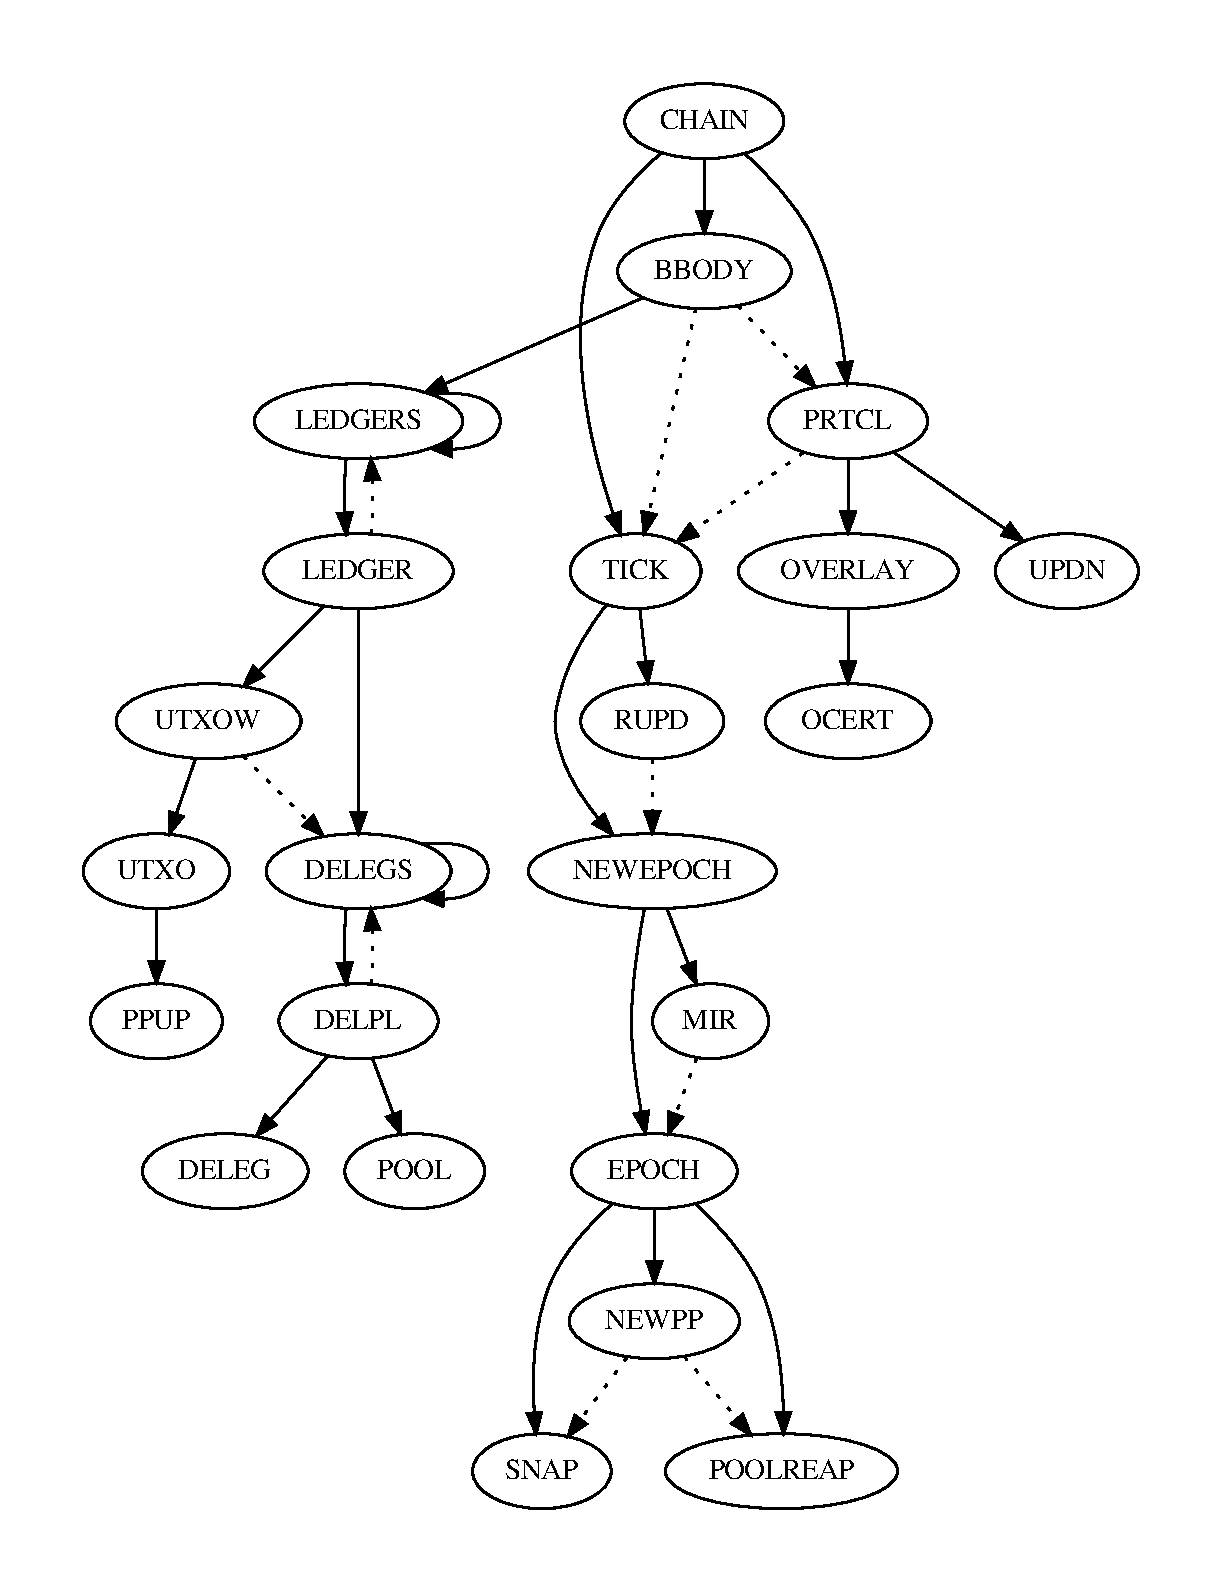
\includegraphics[width=\textwidth]{rules}
  \caption{STS Rules, Sub-Rules and Dependencies}
  \label{fig:sts-rules-dependencies}
\end{figure}

%%% Local Variables:
%%% mode: latex
%%% TeX-master: "ledger-spec"
%%% End:

\section{Formal Properties}
\label{sec:properties}

This appendix collects the main formal properties that the new ledger rules are expected to satisfy.
Note here that in every property in this section we consider a only phase-1 valid
transactions, ie. ones that can indeed get processed.

\begin{enumerate}[label=P{\arabic*}:\ ]
\item
  \emph{Consistency with Shelley.}
  \begin{itemize}
    \item properties 15.6 - 15.16 (except 15.8 and 15.13) hold specifically in the $\fun{txValTag}~tx~=~\True$ case, because
    the calculations refer to the UTxO as if it was updated by a scripts-validating transaction
    \item other properties hold as-is
  \end{itemize}

\item
  \emph{Consistency with Multi-Asset.}
  \begin{itemize}
    \item properties 8.1 and 8.2 hold specifically in the $\fun{txValTag}~tx~=~\True$ case, because
    the calculations refer to the UTxO as if it was updated by a scripts-validating transaction
    \item other properties hold as-is
  \end{itemize}
\end{enumerate}


\begin{definition}
  For a state $s$ that is used in any subtransaction of
  $\mathsf{CHAIN}$, we define $\Utxo(s) \in \UTxO$ to be the $\UTxO$
  contained in $s$, or an empty map if it does not exist. This is
  similar to the definition of $\Val$ in the Shelley specification.

  Similarly, we also define $\field_{v}~(s)$ for the field $v$ that is part of
  the ledger state $s$, referenced by the typical variable name (eg. $\var{fees}$
  for the fee pot on the ledger).
\end{definition}

We also define a helper function $\varphi$ as follows:
\[\varphi(x, tx) :=
  \begin{cases}
    x & \fun{txValTag}~tx = \True \\
    0 & \fun{txValTag}~tx = \False
  \end{cases}\]
This function is useful to distinguish between the two
cases where a transaction can mint tokens or not, depending on whether
its scripts validate.

\begin{property}[General Accounting]
  \label{prop:pov}
  The \emph{general accounting} property in Alonzo encompasses two parts
  \begin{itemize}
    \item preservation of value property expressed via the $\fun{produced}$ and $\fun{consumed}$
    calculations, applicable for transactions with $\fun{txValTag}~tx~=~\True$, which
    is specified as in the ShelleyMA POV.
    \item the preservation of value for $\fun{txValTag}~tx~=~\False$, when
    only the collateral fees are collected into the fee pot.
  \end{itemize}

Both of these are expressed in the following lemma.

\begin{lemma}
  For all environments $e$, transactions $tx$ and states $s, s'$, if
  \begin{equation*}
    e\vdash s\trans{utxos}{tx}s'
  \end{equation*}
  then
  \begin{equation*}
    \Val(s) + \varphi(\fun{mint}~(\fun{txbody}~tx), tx) = \Val(s')
  \end{equation*}
\end{lemma}

\begin{proof}
  In the case that $\fun{txValTag}~tx = \True$ holds, the proof is
  identical to the proof of Lemma 9.1 of the multi-asset
  specification. Otherwise, the transition must have been done via the
  $\mathsf{Scripts-No}$ rule, which removes
  $\fun{collateral}~(\fun{txbody}~tx)$ from the UTxO, and increases the fee pot by the amount of the sum of Ada in the
  collateral UTxO entries. The value contained in $s$ is not changed.

  Note that in the $\fun{feesOK}$ function, there is a check that verifies
  that, in the case that there are phase-2 scripts, there are no non-Ada tokens in the UTxOs
  which the collateral inputs reference, so non-Ada tokens do not get minted, burned, or transferred
  in this case.
\end{proof}
\end{property}

\begin{property}[Extended UTxO Validation]
  \label{prop:fees-only}

  If a phase-1 valid transaction extends the UTxO, all its scripts validate
  (i.e. $\fun{txValTag}~tx = \True$).

  If a transaction is accepted and marked as paying collateral only
  (i.e. $\fun{txValTag}~tx = \False$), then the only change to the ledger
  when processing the transaction is that the collateral inputs
  are moved to the fee pot. In particular, it does not extend the UTxO.

  \begin{lemma}
    For all environments $e$, transactions $tx$ and states $s, s'$, if  and
    \begin{equation*}
      e\vdash s\trans{ledger}{tx}s'
    \end{equation*}
    then
    \[\Utxo(s') \nsubseteq \Utxo(s)~\Rightarrow~\fun{txValTag}~tx = \True \]

    Also,
    \[\fun{txvaltag}~tx = \False~ \Rightarrow~\]
    \begin{itemize}
      \item $ \field_{v}~(s') = \field_{v}~(s) \text{ for all } v~\neq~{fees}, ~v~\neq~{utxo}$
      \item $\field_{fees}~(s') = \field~\var{fees}~(s) + \fun{coin}~(\Val~(\fun{collateral}~{tx} \subtractdom \Utxo(s)))$
      \item $\Utxo(s') = \fun{collateral}~{tx} \subtractdom \Utxo(s)$
    \end{itemize}
  \end{lemma}

  \begin{proof}
    A ledger UTxO update is specified explicitly only by the $\mathsf{UTXOS}$ transition,
    and propagated (ie. applied as-specified) to a chain-state update via the
    $\mathsf{UTXO}$ and $\mathsf{UTXOW}$ transitions.

    The only case in which the $\mathsf{UTXOS}$ transition adds entries to the UTxO
    map is in the $\mathsf{Scripts-No}$ rule, when $\fun{txValTag}~tx = \True$.
    Adding entries to the UTxO map implies exactly that the updated map is not a
    submap of the original, so we get that

    \[\Utxo(s') \nsubseteq \Utxo(s)~\Rightarrow~\fun{txValTag}~tx = \True \]

   In the case that $\fun{txValTag}~tx = \False$, $\mathsf{LEDGER}$ calls the rule
   that does not update $\DPState$ at all, only the $\UTxOState$. This state update is specified
   in the $\mathsf{UTXOS}$ transition (and applied via the $\mathsf{UTXO}$ and $\mathsf{UTXOW}$ transitions).

   The only parts of the state that are updated are
   \begin{itemize}
     \item the fee pot, which is increased by the amount of the sum of Ada in the
     collateral UTxO entries, and
     \item the UTxO, where the collateral entries
     are removed.
   \end{itemize}
  \end{proof}
\end {property}

\begin{property}[Validating when No NN Scripts]
  \label{prop:is-valid}

Whenever a valid transaction does not have any phase-2 scripts, its
$\fun{txValTag} = \True$.

\begin{lemma}
  For all environments $e$, transactions $tx$ and states $s, s'$ such that
  \begin{equation*}
    e\vdash s\trans{ledger}{tx}s',
  \end{equation*}
  If $\range (\fun{txscripts}~tx) \cap \ScriptPhTwo = \emptyset$
  then $\fun{txValTag} = \True$.
\end{lemma}
\begin{proof}
  With the same argument as previously, we only need to discuss the
  equivalent claim for the $\mathsf{UTXOS}$ transition. Under these
  assumptions, $\var{sLst}$ is an empty
  list. Thus $\fun{evalScripts}~sLst = \True$, and the transition rule
  had to be $\mathsf{Scripts{-}Yes}$.
\end{proof}
\end{property}

\begin{property}[Paying fees]
  \label{prop:pay-fees}

In the case that all phase-2 scripts in a transaction validate, the transaction pays
at least the minimum transaction fee amount into the fee pot. In the case that
some do not validate, it must pay at least the percentage of the minimum fee
the collateral is required to cover.

\begin{lemma}
  For all environments $e$, transactions $tx$ and states $s, s'$ such that
  \begin{equation*}
    e\vdash s\trans{ledger}{tx}s'
  \end{equation*}
  The following holds : \\
  $\field_{fees}~(s')~\geq~\field_{fees}~(s)~+
  \begin{cases}
    \fun{minfee}~{tx} & \fun{txValTag} = \True \\
    \fun{quot}~(\fun{collateralPercent}~(\field_{pp}~(s)))~*~(\fun{minfee}~{tx})~100 & \fun{txValTag} = \False\\
  \end{cases}$.
\end{lemma}
\begin{proof}
  The fee pot is updated by the $\mathsf{Scripts{-}Yes}$ and the $\mathsf{Scripts{-}No}$
  rules, one of which is necessarily called by a valid transaction via the sequence
  of transitions called in the order $\mathsf{LEDGER}, \mathsf{UTXOW}, \mathsf{UTXO}, \mathsf{UTXOS}$.

  The $\mathsf{Scripts{-}Yes}$ rule (i.e. $\fun{txValTag} = \True$)
  transfers the amount of Lovelace in the $\fun{txfee}$ field of the
  transaction to the fee pot, which is checked to be at least the $\fun{minfee}$
  by $\fun{feesOK}$ in the $\mathsf{UTXO}$ transition. So, we get

  \[\field_{fees}~(s')~=~\field_{fees}~(s)~+~\fun{txfee}~{tx}~\geq~\field_{fees}~(s)~+~\fun{minfee}~{tx}\]

  The $\mathsf{Scripts{-}No}$ rule (i.e. $\fun{txValTag} = \False$) removes the
  $\fun{collateral}$ inputs from the
  UTxO, and adds the balance of these realized inputs to the fee pot.

  \[\field_{fees}~(s')~=~field_{fees}~(s)~+~\fun{ubalance}~(\fun{collateral}~{txb} \restrictdom \var{utxo})\]

  We can conclude that $\fun{txrdmrs}$ is non-empty whenever $\fun{txValTag} = \False$
  from the following observations :
  \begin{itemize}
    \item $\fun{txValTag} = \False$ whenever $\fun{evalScripts}$ fails.
    \item $\fun{evalScripts}$ is a $\wedge$-fold over a list of scripts and
    their inputs, containing all scripts that need to be run to validate this transaction
    \item All phase-1 scripts must succeed, as this is checked in phase-1 validation (UTXOW
    rule check). Therefore,
    $\fun{evalScripts}$ encounters a failing script which is phase-2.
    \item All phase-2 scripts necessarily have an associated redeemer attached to the
    transaction (UTXOW rule check)
  \end{itemize}

  See Property~\ref{prop:fixed-inputs} for more details on what inputs $\fun{evalScripts}$ has,
  and what we can say about the outcome of its computation with respect to its inputs.

  The $\fun{feesOK}$ check enforces that if a transaction has a non-empty
  $\fun{txrdmrs}$ field, the balance of the realized collateral inputs
  (which $\field_{fees}~(s)$ is increased by as part of processing $tx$) is

  \[\fun{ubalance}~(\fun{collateral}~{txb} \restrictdom \var{utxo})~\geq~\fun{quot}~(\txfee~{txb} * (\fun{collateralPercent}~pp))~100\]

  which, since $\txfee~{txb}~\geq~\fun{minfee}~{txb}$, gives

  \[ \geq~\fun{quot}~(\fun{minfee}~{txb} * (\fun{collateralPercent}~pp))~100)) \]

  where $\fun{txbody}~{tx}~=~{txb}$. This shows that the total collateral that gets
  moved into the fee pot from the UTxO by the $\mathsf{Scripts{-}No}$ rule is at
  least the minimum transaction fee scaled by the collateral percent parameter.

  \[\field_{fees}~(s')~\geq~\field_{fees}~(s)~+~\fun{quot}~(\fun{minfee}~{txb} * (\fun{collateralPercent}~pp))~100))\]
\end{proof}

An immediate corollary to this property is that when the $\fun{collateralPercent}$ is set to 100 or more,
the transaction always pays at least the minimum fee. This, in turn, implies that it
pays at least the fee that it has stated in the $\fun{txfee}$ field.

\begin{corollary}
  For all environments $e$, transactions $tx$ and states $s, s'$ such that
  \begin{equation*}
    e\vdash s\trans{ledger}{tx}s'~~\wedge~~\fun{collateralPercent}~(\field_{pp}~(s)) \geq 100
  \end{equation*}
  The following holds :
  \[\field_{fees}~(s')~\geq~\field_{fees}~(s)~+~\fun{minfee}~{tx} \]
\end{corollary}

\begin{proof}
  In both two cases in the lemma above, the $\field_{fees}$ field in the ledger state
  is increased by at least $\fun{minfee}~{tx}$ :
  \begin{itemize}
    \item when $\fun{txValTag} = \True$, the lemma states already that
    \[\field_{fees}~(s')~\geq~\field_{fees}~(s)~+~\fun{minfee}~{tx}\]
    \item when $\fun{txValTag} = \False$, we have
    $ \field_{fees}~(s')~\geq~\field_{fees}~(s)~+~\fun{quot}~(\fun{minfee}~{txb} * (\fun{collateralPercent}~pp))~100$ \\
    $~~~\geq~\field_{fees}~(s)~+~\fun{quot}~(\fun{minfee}~{tx}~*~100)~100$ \\
    $~~~=~\field_{fees}~(s)~+~\fun{minfee}~{tx}$
  \end{itemize}
\end{proof}

\end{property}

\begin{property}[Correct tag]
  \label{prop:correct-tag}

The $\fun{txValTag}~tx$ tag of a phase-1 valid transaction must match the result of the $\fun{evalScripts}$
function for that transaction.

\begin{lemma}
  For all environments $e$, transactions $tx$ and states $s, s'$ such that
  \begin{equation*}
    e\vdash s\trans{utxos}{tx}s',
  \end{equation*}
  The following holds :
    \[\fun{txValTag}~tx ~=~ \fun{evalScripts}~{tx}~{sLst} \]
  where
  \[ \var{sLst} \leteq \fun{collectTwoPhaseScriptInputs}~\mathsf{EI}~\mathsf{SysSt} ~\field_{pp}(s)~\var{tx}~ \Utxo(s) \]
\end{lemma}
\begin{proof}
  Inspecting the $\mathsf{Scripts{-}Yes}$ and the $\mathsf{Scripts{-}No}$ rules of the $\mathsf{UTXOS}$ transition,
  we see that both the $\fun{txValTag}$ and the result of $\fun{evalScripts}$
  are $\True$ in the former, and $\False$ in the latter.
\end{proof}
\end{property}

\begin{property}[Replay protection]
  \label{prop:replay}

A transaction always removes at least one UTxO entry from the ledger, which provides
replay protection.

\begin{lemma}
  For all environments $e$, transactions $tx$ and states $s, s'$ such that
  \begin{equation*}
    e\vdash s\trans{ledger}{tx}s',
  \end{equation*}
  The following holds : $\Utxo~(s)~\nsubseteq~\Utxo~(s')$.
\end{lemma}
\begin{proof}
  The UTxO is updated by the $\mathsf{Scripts{-}Yes}$ and the $\mathsf{Scripts{-}No}$
  rules, on of which is necessarily called by a valid transaction. Both of these
  rules remove UTxOs corresponding to a set of inputs.

  In both cases, there is a check that the removed inputs set is non-empty.
  The $\mathsf{Scripts{-}Yes}$ rule of the $\mathsf{UTXOS}$ transition
  removes the UTxOs associated with the input set $\fun{txinputs}~{tx}$ from the ledger.
  The $\fun{txinputs}~{tx}$ set must be non-empty because there is a check in the
  $\mathsf{UTXO}$ rule (which calls $\mathsf{UTXOS}$) that ensure this is true.

  For the $\mathsf{Scripts{-}No}$ rule of the $\mathsf{UTXOS}$ transition
  removes the UTxOs associated with the input set $\fun{collateral}~{tx}$ from the ledger.
  The $\fun{collateral}~{tx}$ set must be non-empty because
  the $\fun{feesOK}$ function (called by the same rule that calls $\mathsf{UTXO},
  \mathsf{UTXOS}$) ensures that in the case that the $tx$ contains phase-2 scripts,
  $\fun{collateral}~{tx}$ must be non-empty.

  Note that by property~\ref{prop:is-valid}, phase-2 scripts must always be present
  if $\fun{txValTag}~tx = \False$ (that is, whenever $\mathsf{Scripts{-}No}$ rule is used).
\end{proof}
\end{property}

\begin{property}[UTxO-changing transitions]
  \label{prop:utxo-change}

The $\mathsf{UTXOS}$ transition fully specifies the change in the ledger $\UTxO$
for each transaction.

\begin{lemma}
  For all environments $e$, transitions $\mathsf{TRNS}$, transactions $tx$ and states $s, s'$ such that
  \begin{equation*}
    e\vdash s\trans{trns}{tx}s'
  \end{equation*}
  The following holds :
  \begin{equation*}
    \Utxo(s) \neq \Utxo(s')~\Rightarrow~e'\vdash u\trans{utxos}{tx}u'
  \end{equation*}
  where $\Utxo(s) = \Utxo(u)~\wedge~\Utxo(s') = \Utxo(u')$ for some environment $e'$,
  and states $u, u'$.
\end{lemma}
\begin{proof}
  By inspecting each transition in this specification, as well as those inherited from the
    Shelley one, we see that a non-trivial update from the UTxO of $s$ to that of $s'$
    must be done by $\mathsf{UTXOS}$. Every other transition that changes the UTxO and
    has a signal of type $\Tx$ only applies the $\mathsf{UTXOS}$.
\end{proof}
\end{property}

\begin{property}[Deterministic script evaluation]
  \label{prop:fixed-inputs}

The deterministic script evaluation property, also stated as
"script interpreter arguments are fixed", is a property of the Alonzo ledger
that guarantees that the outcome of phase-2 script validation in a (phase-1 valid) transaction
depends only on the contents of that transaction, and not on when, by who, or in what
block that transaction was submitted.

For this property, we make some assumptions about things that are outside the scope of this specification :

\begin{itemize}
  \item The Plutus script
  interpreter is a pure function that receives only the arguments provided by the ledger when it is
  invoked by calling the $\fun{runPLCScript}$ function. We assume that this is
  also true in an implementation. In particular, the interpreter does not
  obtain any system randomness, etc.

  \item We do not need to check here that the hashes that are the keys of the
  $\fun{txscripts}$ and $\fun{txdats}$ fields match the computed hashes of the scripts and
  datum objects they index. This is because these hashes must be computed as part of
  the deserialization of a transaction (see the CDDL specification),
  instead of being transmitted as part of the transaction and then checked. We
  assume these hashes are correct.

  \item We assume that the consensus
  function $\fun{epochInfoSlotToUTCTime}$ for converting a slot interval into a
  system time interval is deterministic.

  \item We assume that the two global
  constants, $\EpochInfo$ and $\SystemStart$, which it also takes as parameters,
  cannot change within the span of any interval for which $\fun{epochInfoSlotToUTCTime}$
  is able to convert both endpoints to system time.
\end{itemize}

The assumptions above are implicit in the functional style of definitions in this
specification, but they are worth pointing out for implementation.
With these assumptions in mind, we can say that
script evaluation is deterministic.

We split this result into a lemma and its corollary :

\begin{itemize}
  \item First, we demonstrate that all the scripts and their arguments that are
  collected for phase-2 validation are the same for two phase-1 valid transactions with the same body,
  independent of the (necessarily valid) ledger state to which they are being applied

  \item Second, we derive the corollary that under the same validity assumptions,
  phase-2 validation results in the same outcome for both transactions
\end{itemize}

\begin{lemma}
  \label{lem:inputs}
  For all environments $e, e'$, transactions $tx, tx'$ and states $s, s', u, u'$ such that
  $e$ and $s$ are subsets of fields of some valid chain state $c$, and
  $e'$ and $s'$ are subsets of fields of some valid chain state $c'$,

  \begin{equation*}
    e\vdash s\trans{ledger}{tx}s', \\
    e'\vdash u\trans{ledger}{tx'}u', \\
    \txbody{tx} = \txbody{tx'}
  \end{equation*}

  The following holds :

  \[\fun{toSet}~(\fun{collectTwoPhaseScriptInputs}~\mathsf{EI}~\mathsf{SysSt} ~\field_{pp}(s)~\var{tx}~ \Utxo(s))\]
  \[ = \]
  \[\fun{toSet}~(\fun{collectTwoPhaseScriptInputs}~\mathsf{EI}~\mathsf{SysSt} ~\field_{pp}(u)~\var{tx'}~ \Utxo(u))\]

\end{lemma}
\begin{proof}

    The $\fun{collectTwoPhaseScriptInputs}$
    function (see \ref{fig:functions:script2})
    constructs a list where each entry contains a Plutus script
    and the arguments passed to the interpreter for its evaluation.

    To show that $\fun{collectTwoPhaseScriptInputs}$ returns a list containing
    the same elements for both $tx$ and $tx'$, we observe that
    the set of elements from which this list is produced via $\fun{toList}$
    is generated using the following functions, as well as set comprehension
    and list operations.
    We demonstrate that the functions used in this definition
    produce the same output for $tx$ and $tx'$, as all the data they
    inspect is fixed by the transaction body :

    \begin{itemize}
      \item $\fun{scriptsNeeded}$ : The $\PolicyID$, $\AddrRWD$, and $\DCert$ data
      output by this function as the second term of the hash-purpose pair
      is obtained directly from the $\fun{mint}$, $\fun{txwdrls}$,
      $\fun{txcerts}$ fields of the transaction, which are all fixed by the
      body of the transaction. These types of script purposes all include
      the hash of the validating script.

      The only other data this function inspects is the UTxO entries associated
      with the $\fun{txinputs}$ (passed via the $\UTxO$ argument) to get the realized inputs.
      We know that the UTxO is a field in a valid chain state for both the phase-1 valid
      transactions $tx$ and
      the $tx'$ ($\Utxo(s)$ and $\Utxo(u)$, respectively). This means that the $\TxId$
      in each input present in either UTxO is a hash of the body of the transaction
      containing the $\TxOut$ part of the UTxO entry indexed by that input. The
      order of the outputs is also fixed by the body, which fixes the $\Ix$ of
      the entry.

      A different value in output part of the UTxO entry (or a different order of
      outputs) would necessarily imply
      that the hash of the body containing that output must be different.
      Therefore, for all Plutus script-locked realized inputs of either transaction,
      the script hash in the payment credential of the address
      (and, by the same argument, the datum hash) are fixed by the inputs in body of the
      transaction, despite not being explicitly contained in it. We then get that

      \[ \fun{scriptsNeeded}~\Utxo(s)~(\txbody{tx}) = \fun{scriptsNeeded}~\Utxo(u)~(\txbody{tx'}) \]

      \item $\fun{getDatum}$ : In the case the script purpose
      is of the input type, the datum this function returns is one that
      is associated with the corresponding realized input. More precisely, it is the datum whose
      hash is specified in the realized input, and is looked up by hash in the $\fun{txdats}$
      transaction field. If there is no datum hash in the realized input, or the script purpose
      is of a non-input type, the empty list is returned.

      The $\mathsf{UTXOW}$ rule checks that the transaction is carrying all datums corresponding
      to its realized inputs. Since the inputs (and realized inputs) are the same
      for $tx$ and $tx'$ (fixed by the body), this guarantees that
      of the datum hashes in the realized inputs (and therefore, their preimages)
      are the same as well.

      \item $\fun{txscripts}$ : in the $\mathsf{UTXOW}$ rule, there is a check that all the
      script preimages of the script hashes returned by the $\fun{scriptsNeeded}$
      function must be present in this field.

      \item $\fun{indexedRdmrs}$ : like $\fun{scriptsNeeded}$, this function
      examines four fields fixed by the transaction body ($\fun{mint}$, $\fun{txwdrls}$,
      $\fun{txcerts}$, and $\fun{txinputs}$).
      It also looks at data in the $\fun{txrdmrs}$ field, which is fixed
      by the transaction body via the $\fun{scriptIntegrityHash}$
      hash. This is done as follows: the $\mathsf{UTXOW}$ rule verifies that this
      hash-containing field matches the computed hash
      of the preimage constructed from several fields of the transaction,
      including $\fun{txrdmrs}$ (this calculation
      is done by the $\fun{hashScriptIntegrity}$ function).

      \item $\fun{language}$ : this is directly conveyed by the type of a script.

      \item $\fun{costmdls}$ : The hash calculated by the $\fun{hashScriptIntegrity}$
      function and compared to the hash value in the $\fun{scriptIntegrityHash}$ field
      must include in the preimage the current cost models of
      all script languages of scripts carried by the transaction. Recall that
      if a cost model changed between when a transaction was submitted and the
      time at which it was processed, the field and the calculated hash values
      will not match.

      \item $\fun{valContext}$ and $\fun{txInfo}$ :
      The $\fun{valContext}$ function is defined in \ref{sec:txinfo} and is pure.
      All fields of the $\TxInfo$
      structure, with the exceptions listed below,
      are straightforward translations of the corresponding transaction body fields (see \ref{sec:txinfo}) that
      are given no additional arguments,
      and therefore completely determined by $tx$ and $tx'$. The fields not directly
      appearing in the body are :

      \begin{itemize}
        \item $\fun{txInfoInputs}$ : this field contains the realized inputs of
        the transaction which are fixed by the transaction and the unique
        UTxO entries to which the inputs correspond. As explained above,
        accessing information in realized inputs for script evaluation
        does not break determinism.

        \item $\fun{txInfoValidRange}$ : this field contains the transaction
        validity interval as system time (converted from the slot numbers, which are
        used to specify the interval in the transaction body). This conversion is
        done by a function defined in the consensus layer, and takes two global
        constants in addition to the slot interval itself. Since the slot interval
        conversion function $\fun{epochInfoSlotToUTCTime}$ necessarily
        succeeds if both $tx$ and $tx'$ pass phase-1 validation, the additional
        global constant arguments must be the same (by assumption). The determinism of this conversion
        is one of the assumptions of this property, and thus gives the same output
        for both transactions.

        \item $\fun{txInfoData}$ : this field is populated with the datums (and their
        hashes) in the transaction field $\fun{txdats}$, which are fixed by the body
        via the $\fun{scriptIntegrityHash}$ field.

        \item $\fun{txInfoId}$ : this field contains the hash of the transaction body,
        which is clearly the same for transactions with the same body.
      \end{itemize}

      Therefore, each field of the $\TxInfo$ structure is
      the same for two transactions with the same body, ie.

      \[ \fun{txInfo}~\PlutusVI~\Utxo(s)~\var{tx} = \fun{txInfo}~\PlutusVI~\Utxo(u)~\var{tx'}\]

    \end{itemize}
\end{proof}

We can now make the general statement about evaluation of all scripts done in
phase-2 validation : for any phase-1 valid transactions with the same body,
the outcome of phase-2 script evaluation is the same. We make the same assumptions
as in Lemma \ref{lem:inputs}.

\begin{corollary}
  For all environments $e, e'$, transactions $tx, tx'$ and states $s, s', u, u'$ such that
  \begin{equation*}
    e\vdash s\trans{ledger}{tx}s', \\
    e'\vdash u\trans{ledger}{tx'}u', \\
    \txbody{tx} = \txbody{tx'}
  \end{equation*}
  The following holds :

  \[\fun{evalScripts}~{tx}~ (\fun{collectTwoPhaseScriptInputs}~\mathsf{EI}~\mathsf{SysSt} ~\field_{pp}(s)~\var{tx}~ \Utxo(s))\]
  \[ = \]
  \[\fun{evalScripts}~{tx'}~ (\fun{collectTwoPhaseScriptInputs}~\mathsf{EI}~\mathsf{SysSt} ~\field_{pp}(u)~\var{tx'}~ \Utxo(u))\]

\end{corollary}

\begin{proof}
  Let us consider the use of arguments of $\fun{evalScripts}$ (see Figure \ref{fig:functions:script2}).
  The first argument (of type $\Tx$) is only inspected in the case that the script $sc$ (the first element
    in the pair at the head of the list of script-arguments pairs is a phase-1 script. Since all phase-1 scripts
    are checked in phase one of validation (see \ref{fig:rules:utxow-alonzo}) by calling $\fun{validateScript}$
    on all scripts attached to the transaction. For this to apply to $sc$, we must also show
    that $sc$ is a script attached to the transaction (see the second argument explanation).
    Note also that the $tx$ argument passed to $\fun{evalScripts}$ at the use site (in the $\mathsf{UTXOS}$ transition)
    is the same, unmodified $tx$ as is the signal for the LEDGER transition. We verify this by inspecting
    the sequence of transitions through which it is propagated
    ($\mathsf{UTXOS}$, $\mathsf{UTXO}$, $\mathsf{UTXOW}$, and $\mathsf{LEDGER}$), and their signals.

    This allows us to conclude that at every step of the iteration over the script-arguments pairs list,
    the first argument to $\fun{evalScripts}$,

    \begin{itemize}
      \item has no impact on the outcome of script evaluation in the case the script
      being validated at this step is phase-2, as it is completely ignored, and,

      \item because $\fun{collectTwoPhaseScriptInputs}$ filters out all phase-1 scripts,
      is, in fact, ignored always.
    \end{itemize}

    The second argument to $\fun{evalScripts}$, ie. the list of scripts and their arguments,
    has already been shown to contain the same tuples for both transactions in the lemma above.
    The order of the list does not affect the validation outcome, since the interpreter is run
    on each tuple of a script and its arguments independently of all other tuples in the list.
    The function $\fun{evalScripts}$ is a $\wedge$-fold over the list. Thus, we may ignore the order
    of the elements in the generated list as it does not affect the evaluation outcome.

    From this we may conclude that the outcome of both phase-1 and phase-2 script evaluations
    at each step of $\fun{evalScripts}$ must be the same for $tx$ and $tx'$. Therefore,
    the $\wedge$-fold of them done by $\fun{evalScripts}$ also produces the same outcome
    for both transactions.

\end{proof}
\end{property}


\begin{enumerate}
\item
  \emph{Commutativity of Translation.} Translate, then apply to Alonzo ledger is
  the same as apply to MA ledger, then translate the ledger.
\item
  \emph{Zero ExUnits.} If a script is run (there’s a redeemer/exunits) , it will fail with 0 units
\item
  \emph{Cost Increase.} if a transaction is valid, it will remain valid if you increase the execution units
\item
  \emph{Cost Lower Bound.} if a transaction contains at least one valid script, it must have at least one execution unit
\item
  \emph{Tx backwards Compatibility.} Any transaction that was accepted in a previous version of the ledger rules
    has exactly the same cost and effect, except that the transaction output is extended.
\item \emph{Run all scripts.} All scripts attached to a transaction are run
\item
  ... \todo{Anything else?}
\end{enumerate}

\section{Leader Value Calculation}
\label{sec:leader-value-calc}

This section details how we determine whether a node is entitled to lead (under
the Praos protocol) given the output of its verifiable random function
calculation.

\begin{figure}
  \emph{Values associated with the leader value calculations}
  \begin{equation*}
  \begin{array}{r@{~\in~}lr}
    \var{certNat} & \{n | n \in \N, n \in [0,2^{512})\} & \text{Certified natural value from VRF} \\
    \var{f} & [0,1] & \text{Active slot coefficient} \\
    \sigma & [0,1] & \text{Stake proportion}
  \end{array}
  \end{equation*}
\end{figure}

\subsection{Computing the leader value}

The verifiable random function gives us a 64-byte random output. We interpret
this as a natural number $\var{certNat}$ in the range $[0,2^{512})$.

\subsection{Node eligibility}

As per \cite{ouroboros_praos}, a node is eligible to lead when its leader value
$p < 1 - (1 - f)^\sigma$. We have

\begin{align*}
  p & < 1 - (1 -f)^\sigma \\
  \iff \left(\frac{1}{1-p}\right) & < \exp{(-\sigma \cdot \ln{(1-f)})}
\end{align*}

The latter inequality can be efficiently computed through use of its Taylor
expansion and error estimation to stop computing terms once we are certain that
the result will be either above or below the target value.

We carry out all computations using fixed precision arithmetic (specifically, we
use 34 decimal bits of precision, since this is enough to represent the fraction
of a single lovelace.)

As such, we define the following:

\begin{align*}
  p & = \frac{\var{certNat}}{2^{512}} \\
  q & = 1 - p \\
  c & = \ln{(1 - f)}
\end{align*}

and define the function \textit{checkLeaderVal} as follows:

\begin{equation*}
  \fun{checkLeaderVal}~\var{certNat}~\sigma~\var{f} =
    \left\{
      \begin{array}{l@{~}r}
        \mathsf{True}, & f = 1 \\
        \frac{1}{q} < \exp{(-\sigma \cdot c)}, & \text{ otherwise}
      \end{array}
    \right.
\end{equation*}

\section{Errata}
\label{sec:errata}

We list issues found within the Shelley ledger which will be corrected in future eras.

\subsection{Total stake calculation}
\label{sec:errata:total-stake}

As described in \cite[3.4.3]{delegation_design}, stake is sometimes considered
relative to all the delegated stake, and sometimes relative to the
totally supply less the amount held by the reserves.
The former is called active stake, the latter total stake.


The $\fun{createRUpd}$ function from Figure~\ref{fig:rules:reward-update} uses the
current value of the reserve pot, named $\var{reserves}$, to calculate the total stake.
It should, however, use the value of the reserve pot as it was during the previous
epoch, since $\fun{createRUpd}$ is creating the rewards earned during the previous epoch
(see the overview in Section~\ref{sec:reward-overview}).

\subsection{Active stake registrations and the Reward Calculation}
\label{sec:errata:active-accounts-and-reward-calc}

The reward calculation takes the set of active reward accounts as a parameter
(the forth parameter of $\fun{reward}$ in Figure~\ref{fig:functions:reward-calc}).
It is only used at the end of the calculation for filtering out unregistered accounts.
Therefore, if a stake credential is deregistered just before the reward calculation starts,
it cannot reregister before the end of the epoch in order to get the rewards.
The time within the epoch when the reward calculation starts should not make any difference.
Note that this does not affect the earnings that stake pools make from their margin,
since each pool's total stake is summed before filtering.
The solution is to not filter by the current active reward accounts, since rewards for
unregistered accounts go to the treasury already anyway.

\subsection{Stability Windows}
\label{sec:errata:stability-windows}

The constant $RandomnessStabilisationWindow$ was intended to be used only
for freezing the candidate nonce in the $\mathsf{UPDN}$ rule
from Figure~\ref{fig:rules:update-nonce}.
This was chosen as a good value for both Ouroboros Praos and Ouroboros Genesis.
The implementation mistakenly used the constant in the $\mathsf{RUPD}$ rule
from Figure~\ref{fig:rules:reward-update}, and used $\StabilityWindow$
in for the $\mathsf{UPDN}$ transition.

The constant $\StabilityWindow$ is a good choice for the $\mathsf{UPDN}$
transition while we remain using Ouroboros Praos, but it will be changed before
adopting Ouroboros Genesis in the consensus layer.

There is no problem with using $RandomnessStabilisationWindow$ for the
$\mathsf{RUPD}$ transition, since anything after $\StabilityWindow$ would work,
but there is no reason to do so.

\subsection{Reward aggregation}
\label{sec:errata:reward-aggregation}

On any given epoch, a reward account can earn rewards by being a member of a stake pool,
and also by being the registered reward account for a stake pool (to receive leader rewards).
A reward account can be registered to receive leader rewards from multiple stake pools.
It was intended that reward accounts receive the sum of all such rewards,
but a mistake caused reward accounts to receive at most one of them.

In Figure~\ref{fig:functions:reward-calc}, the value of $\var{potentialRewards}$ in the
$\fun{rewardOnePool}$ function should be computed using an aggregating union
$\unionoverridePlus$, so that member rewards are not overridden by leader rewards.
Similarly, the value of $\var{rewards}$ in the $\fun{reward}$ function should be computed
using an aggregating union so that leader rewards from multiple sources are aggregated.

This was corrected at the Allegra hard fork.
There were sixty-four stake addresses that were affected,
each of which was reimbursed for the exact amount lost using a MIR certificate.
Four of the stake address were unregistered and had to be re-registered.
The unregistered addresses were reimbursed in transaction
\newline
$a01b9fe136e5703668c9c7776a76cc8541b84824635d237e270670a8ca56a392$,
and the registered addresses were reimbursed in transaction
\newline
$8cab8049e3b8c4802d7d11277b21afc74056223a596c39ef00e002c2d1f507ad$.

\subsection{Byron redeem addresses}
\label{sec:errata:byron-redeem-addresses}

The bootstrap addresses from Figure~\ref{fig:defs:addresses} were not intended
to include the Byron era redeem addresses
(those with addrtype 2, see the Byron CDDL spec).
These addresses were, however, not spendable in the Shelley era.
At the Allegra hard fork they were removed from the UTxO
and the Ada contained in them was returned to the reserves.


\clearpage

\addcontentsline{toc}{section}{References}
\bibliographystyle{habbrv}
\bibliography{references}

\clearpage
\begin{appendix}
  \section{Cryptographic Details}
\label{sec:crypto-details}

\subsection{Hashing}
We present the (informal) properties of cryptographically safe hash functions:
\begin{description}
\item[Preimage resistance] It should be hard to find a message with a given hash value.
\item[Second preimage resistance] Given one message, it should be hard to find another message with the same hash value.
\item[Collision resistance] It should be hard to find two messages with the same hash value. 
\end{description}

\noindent In practice, several cryptographic protocols use hash functions as random oracles. 
However, the properties of our scheme do not depend on it.  

The hashing algorithm we use for all verification keys and multi-signature scripts is BLAKE2b-224\footnote{Note that for the signature 
and verification algorithms, as well as the proving and verification algorithms of VRFs, we use the hash function as defined in the IETF standard (see Section~\ref{sec:app-addresses} and Section~\ref{sec:app-vrf}).}.
Explicitly, this is the payment and stake credentials (Figure~\ref{fig:defs:addresses}),
the genesis keys and their delegates (Figure~\ref{fig:ts-types:pp-update}),
stake pool verification keys (Figure~\ref{fig:delegation-transitions}),
and VRF verification keys (Figure~\ref{fig:delegation-defs}). 
The only property we require of this hash function is that of Second Preimage resistance. Given the hash of verification key or multi-signature script, it should be hard to find a different key or script with the same hash. 

Everywhere else we use BLAKE2b-256. In this case we do require second preimage resistance and collision resistance. We use the output of these hash functions to produce signatures (see Figure~\ref{fig:rules:utxow-shelley}), meaning that if an adversary can find two messages with the same hash, it could break the intended EUF-CMA (Existentially UnForgeable against a Chosen Plaintext Attack) property of the underlying signature scheme. 
 
In the CDDL specification in Appendix~\ref{sec:cddl},
$\mathsf{hash28}$ refers to BLAKE2b-224 and
and $\mathsf{hash32}$ refers to BLAKE2b-256.
BLAKE2 is specified in RFC 7693 \cite{rfcBLAKE2}.

\subsection{Addresses}
\label{sec:app-addresses}
The \fun{sign} and \fun{verify} functions from Figure~\ref{fig:crypto-defs-shelley}
use Ed25519. See \cite{rfcEdDSA}.

\subsection{KES}
The \fun{sign_{ev}} and \fun{verify_{ev}} functions from Figure~\ref{fig:kes-defs-shelley}
use the iterated sum construction from Section 3.1 of \cite{cryptoeprint:2001:034}.
We allow up to $2^7$ key evolutions, which is larger than the maximum number
of evolutions allow by the spec, \MaxKESEvo, which will be set to $90$.
See Figure~\ref{fig:rules:ocert}.

\subsection{VRF}
\label{sec:app-vrf}
The \fun{verifyVrf} function from Figure~\ref{fig:defs-vrf}
uses ECVRF-ED25519-SHA512-Elligator2 as described in the draft IETF specification
\cite{rfcVRFDraft}.

More generally, we expect the following properties from a Verifyable Random Function: 
\begin{description}
\item[Full uniqueness] For any fixed public VRF key and for \textit{any} input seed, there is a unique VRF output that can be proved valid. 
\item[Full collision resistance] It should be computationally infeasible to find two distinct VRF inputs that have the same VRF output, even if the adversary knows the private key. 
\item[Pseudorandomness] Assuming the public-private key pair has been generated honestly, the VRF hash output on any adversarially-chosen VRF input looks indistinguishable from random for a computationally bounded adversary who does not know the private key. 
\end{description}

\subsection{Multi-Signatures}
As presented in Figure~\ref{fig:types-msig}, Shelley realizes multi-signatures 
in a native way, via a script-like DSL. One defines the conditions required to 
validate a multi-signature, and the script takes care of verifying the 
correctness of the request. It does so in a na\"ive way, i.e. checking every 
signature individually. For instance, if the requirement is to have $n$ valid 
signatures out of some set $\mathcal{V}$ of public keys, the na\"ive 
script-based solution checks if: (i) the number of submitted signatures is 
greater or equal to $n$, (ii) the distinct verification keys are part of the set 
$\mathcal{V}$, and (iii) at least $n$ signatures are valid. However, there are 
more efficient ways to achieve this using more advanced multi-signature schemes, 
that allow for aggregating both the signatures and the verification procedure. 
This results in less data to be stored on-chain, and a cheaper verification 
procedure. Several schemes provide these properties~\cite{musigBoneh, musig, 
musig2, pixel}, and we are currently investigating which would be the best fit 
for the Cardano ecosystem. We formally introduce multi-signature schemes.

\sloppy
A multi-signature scheme~\cite{musigs} is defined as a tuple of algorithms 
$\textsf{MS} = (\textsf{MS-Setup}, \textsf{MS-KG}, \textsf{MS-AVK}, 
\allowbreak\textsf{MS-Sign}, \textsf{MS-ASign}, \textsf{MS-Verify)}$ such that 
$\Pi\leftarrow\textsf{MS-Setup}(1^k)$ generates public parameters---where $k$ is 
the security parameter. Given the public parameters, one can generate a 
verification-signing key pair calling, 
$(\mathsf{vk,sk})\leftarrow\textsf{MS-KG}(\Pi)$. A multi-signature scheme 
provides a signing and an aggregate functionality. Mainly
\begin{itemize}
\item $\sigma\leftarrow\textsf{MS-Sign}(\Pi, \mathsf{sk}, m)$, produces a 
signature, $\sigma$, over a message $m$ using signing key $\mathsf{sk}$, and
\item $\tilde{\sigma}\leftarrow\textsf{MS-ASig}(\Pi, m, \mathcal{V, S)}$, where 
given a message $m$, a set of signatures, $\mathcal{S}$, over the message $m$, 
and the corresponding set of verification keys, $\mathcal{V}$, aggregates all 
signatures into a single, aggregate signature $\tilde{\sigma}$. 
\end{itemize}

To generate an aggregate verification key, the verifier calls the function 
$\mathsf{avk}\leftarrow\textsf{MS-AVK}(\Pi, \mathcal{V})$, which given input a 
set of verification keys, $\mathcal{V}$, returns an aggregate verification key 
that can be used for the verification of the aggregate siganture: 
$\textsf{MS-Verify}(\Pi, \mathsf{avk}, m, 
\tilde{\sigma})\in\{\textsf{true},\textsf{false}\}$. 

Note the distinction between multi-signature schemes (as described above) and 
multi-signatures as defined in Figure~\ref{fig:types-msig}. In 
Figure~\ref{fig:types-msig} we allow scripts to consider valid the 
\type{RequireAllOf}, \type{RequireAnyOf} or \type{RequireMOfN} typed signatures. 
In the definition above, given a set of public keys $\mathcal{V}$, a signature 
is considered valid if \textit{all} key owners participate. However, such 
multi-signature schemes together with a simple script-like DSL can achieve the 
properties defined in Figure~\ref{fig:types-msig} while still providing the 
benefits of a simple verification procedure, and a smaller signature size. 

  \section{Binary Address Format}
\label{sec:address-binary}

\newcommand{\binary}[1]{\ensuremath{\mathsf{#1}}}

Excepting bootstrap addresses,
the binary format for every address has a 1-byte header, followed by a payload
(bootstrap addresses use the binary encoding from the Byron era).
The header is composed of two nibbles (two 4-bit segments),
indicating the address type and the network id.

$$
\begin{array}{r@{~=~}l}
    \mathsf{address} & \mathsf{header\_byte}|\mathsf{payload} \\
                     & \mathsf{addr\_type\_nibble}|\mathsf{network\_nibble}|\mathsf{payload}
\end{array}
$$

\subsection{Header, first nibble}
\label{sec:address-binary-header-first-nibble}

The first nibble of the header specifies the type of the address.
Bootstrap addresses can also be identified by the first nibble.

\begin{center}
\begin{tabular}{ |c|c|c|c| }
 \hline
 address type & payment credential & stake credential & header, first nibble \\
 \hline
 \hline
 base address & keyhash      & keyhash    & \binary{0000} \\
 base address & scripthash   & keyhash    & \binary{0001} \\
 base address & keyhash      & scripthash & \binary{0010} \\
 base address & scripthash   & scripthash & \binary{0011} \\
 \hline
 pointer address & keyhash    & ptr & \binary{0100} \\
 pointer address & scripthash & ptr & \binary{0101} \\
 \hline
 enterprise address & keyhash    & - & \binary{0110} \\
 enterprise address & scripthash & - & \binary{0111} \\
 \hline
 bootstrap address & keyhash    & - & \binary{1000} \\
 \hline
 stake address & - & keyhash & \binary{1110} \\
 stake address & - & scripthash & \binary{1111} \\
 \hline
 future formats & ? & ? & \binary{1001}-\binary{1101} \\
 \hline
\end{tabular}
\end{center}

\subsection{Header, second nibble}
\label{sec:address-binary-header-second-nibble}

Excepting bootstrap addresses, the second nibble of the header specifies the network.

\begin{center}
\begin{tabular}{ |c|c| }
 \hline
 network & header, second nibble \\
 \hline
 \hline
 testnets & \binary{0000} \\
 mainnet & \binary{0001} \\
 future networks & \binary{0010}-\binary{1111}\\
 \hline
\end{tabular}
\end{center}

\subsection{Header, examples}
\label{sec:address-binary-header-examples}

On a \textbf{testnet},
the header for a \textbf{pointer} address whose payment credential is a \textbf{keyhash} is:
$$\binary{00000100}$$

On \textbf{mainnet}, the header for a \textbf{pointer} address whose payment credential is a \textbf{keyhash} is:
$$\binary{00010100}$$

On \textbf{mainnet}, the header for a \textbf{pointer} address whose payment credential is a \textbf{scripthash} is:
$$\binary{00010101}$$

\subsection{Payloads}
\label{sec:address-binary-payloads}

The payload for the different address types are as follows:

\begin{center}
\begin{tabular}{ |c|c| }
 \hline
 address type & payload \\
 \hline
 \hline
 base address & two 28-byte bytestrings \\
 \hline
 pointer address & one 28-byte bytestring,
 and three variable-length unsigned integers \\
 \hline
 enterprise address & one 28-byte bytestrings \\
 \hline
 stake address & one 28-byte bytestrings \\
 \hline
\end{tabular}
\end{center}

The variable-length encoding used in pointers addresses is the base-128 representation
of the number, with the most significant bit of each byte indicating continuation
(this is sometimes called a variable-length quantity, or VLQ).
If the significant bit is $1$, then another byte follows.

  \section{Bootstrap Witnesses}
\label{sec:bootstrap-witnesses}

\subsection{Bootstrap Witnesses CBOR Specification}

In the Byron era of Cardano, public keys are transmitted
on chain as extended public keys as specified in \cite{bip32}.
The Shelley era of Cardano does not use extended public keys,
but does use the same cryptographic signing algorithm,
namely Ed25519.

The extended public key consists of 64 bytes,
the first 32 of which corresponds to the public key,
the second 32 of which correpsonds to something called the chain code:

$$\mathsf{extended\_pubkey} = \mathsf{pubkey}|\mathsf{chain\_code}$$

The chaincode is required for constructing bootstrap witnesses.

The CBOR specification of bootstrap witnesses,
named $\mathsf{bootstrap\_witness}$,
is given in
\url{https://github.com/input-output-hk/cardano-ledger/tree/master/eras/shelley/impl/cddl-files}.

In the Shelley era, only pubkey address are supported,
and are named bootstrap addresses.

The bootstrap witness consists of the public key, the signature,
the chain code, and the address attributes.
As explained above, the public key and the signature format
are the same as for all other witnesses in the Shelley era.
The address attributes has the same format as from the Byron era address,
as specified by $\mathsf{addrattr}$ in
\url{https://github.com/input-output-hk/cardano-ledger/blob/master/eras/byron/cddl-spec/byron.cddl}.


\subsection{Bootstrap Address ID Recovery}

The bootstrap address ID, named $\mathsf{addressid}$ in the Byron CDDL
specification above, can be computed as follows.

First construct the following byte string:

$$\mathsf{b} =
  \mathsf{0x830082005840}
  | \mathsf{pubkey\_bytes}
  | \mathsf{chain\_code\_bytes}
  | \mathsf{attributes\_bytes}
$$

The address ID is then obtained by first applying
sha3 256 to $\mathsf{b}$ and then applying blake2b44 to the result.
$$\mathsf{address\_id} =
  \mathsf{blake2b44}(\mathsf{sha3\_256}~\mathsf{b})
$$

  \chapter{CDDL Specification of the Protocol Messages}
\label{CBOR-section}
\hsref{ouroboros-network/test/messages.cddl}
\label{included-cddl}
This Sections contains the CDDL~\cite{cddl} specification
of the binary serialisation format of the network protocol messages.

To keep this Section in close sync with the actual Haskell implementation
the names of the Haskell identifiers have been reused for the corresponding
CBOR types (with the first letter converted to lower case).
Note, that, for readability, the previous Sections used simplified message identifiers,
for example {\tt RequestNext} instead of {\tt msgRequestNext}, etc.
Both identifiers refer to the same message format.

All transmitted messages satisfy the shown CDDL specification.
However, CDDL, by design, also permits variants in the encoding that are not valid in the protocol.
In particular, the notation ${\tt [} ... {\tt ]}$ in CDDL can be used for both fixed-length
and variable-length CBOR-list, while only one of the two encodings is valid in the protocol.
We add comments in specification to make clear which encoding must be used.

Note that, in the case of the request-response mini protocol (Section~ref{request-response-protocol})
there is only one possible kind of message in each state.  This means that
there is no need to tag messages at all and the protocol can directly transmit
plain request and response data.

\lstinputlisting{../../ouroboros-network/test/messages.cddl}

  \section{Implementation of \fun{txSize}}
\label{sec:txSize}

The minimum fee calculation in Figure~\ref{fig:defs:protocol-parameters-helpers}
depends on an abstract $\fun{txSize}$ function.
We have implemented $\fun{txSize}$ as the number of bytes in the CBOR serialization
of the transaction, as defined in Appendix~\ref{sec:cddl}.

  \section{Proofs}
\label{sec:proofs}

\newif\ifproofs
% \proofstrue comment in to include generated proofs

For the proofs we use the automated theorem prover
MetiTarski~\cite{DBLP:journals/jar/AkbarpourP10} which is specialized for proofs
over real arithmetic, including elementary functions.

\begin{proof}
The property~(\ref{prop:minimal-refund}) (p.~\pageref{prop:minimal-refund}) for
the minimal refund can be proven automatically via

\begin{verbatim}
fof(minimal_refund, conjecture,
! [Dmin, Lambda, Delta, Dval] :
((Dmin : (=0,1=) & Lambda > 0 & Delta > 0 & Dval > 0
=>
Dval*Dmin >= 0 &
(Dval * (Dmin + (1 - Dmin) * exp(-Lambda * Delta))) : (=Dval * Dmin, Dval=)))).

fof(floor_lower_upper, conjecture,
! [X] :
(X >= 0 => X - 1 <= floor(X) & floor(X) <= X)).
\end{verbatim}
  \verb|minimal_refund| shows that the resulting value is within the interval
  $[d_{val}\cdot d_{min}, d_{val}]$ and that $d_{val}\cdot d_{min}$ is
  non-negative, while \verb|floor_lower_upper| shows that the floor of a value
  $x$ has an upper bound $x$ and lower bound $x - 1$.

\ifproofs
\begin{verbatim}
SZS output start CNFRefutation for minRefund.tptp
cnf(lgen_le_neg, axiom, (X <= Y | ~ lgen(0, X, Y))).

cnf(leq_left_divide_mul_pos, axiom, (Y * Z < X | X / Z <= Y | Z <= 0)).

cnf(interval_intro, axiom,
    (~ lgen(R, A, X) | ~ lgen(S, X, B) | interval(R, A, S, B, X))).

cnf(interval_elim1, axiom, (~ interval(R, A, S, B, X) | lgen(R, A, X))).

cnf(interval_elim2, axiom, (~ interval(R, A, S, B, X) | lgen(S, X, B))).

cnf(exp_upper_bound_cf2, axiom,
    (0 <= X | ~ lgen(R, (X ^ 2 + 6 * X + 12) / (X ^ 2 - 6 * X + 12), Y) |
     lgen(R, exp(X), Y))).

fof(minimal_refund, conjecture,
    (! [Dmin, Lambda, Delta, Dval] :
       ((interval(0, 0, 0, 1, Dmin) & 0 < Lambda & 0 < Delta & 0 < Dval) =>
        (0 <= Dval * Dmin &
         interval(0, Dval * Dmin, 0, Dval,
                  Dval * (Dmin + (1 - Dmin) * exp(-Lambda * Delta))))))).

fof(subgoal_0, plain,
    (! [Dmin, Lambda, Delta, Dval] :
       ((interval(0, 0, 0, 1, Dmin) & 0 < Lambda & 0 < Delta & 0 < Dval) =>
        0 <= Dval * Dmin)), inference(strip, [], [minimal_refund])).

fof(subgoal_1, plain,
    (! [Dmin, Lambda, Delta, Dval] :
       (((interval(0, 0, 0, 1, Dmin) & 0 < Lambda & 0 < Delta & 0 < Dval) &
         0 <= Dval * Dmin) =>
        interval(0, Dval * Dmin, 0, Dval,
                 Dval * (Dmin + (1 - Dmin) * exp(-Lambda * Delta))))),
    inference(strip, [], [minimal_refund])).

fof(negate_0_0, plain,
    (~ ! [Dmin, Lambda, Delta, Dval] :
         ((interval(0, 0, 0, 1, Dmin) & 0 < Lambda & 0 < Delta &
           0 < Dval) => 0 <= Dval * Dmin)),
    inference(negate, [], [subgoal_0])).

fof(normalize_0_0, plain,
    (? [Delta, Dmin, Dval, Lambda] :
       (0 < Delta & 0 < Dval & 0 < Lambda & Dval * Dmin < 0 &
        interval(0, 0, 0, 1, Dmin))),
    inference(canonicalize, [], [negate_0_0])).

fof(normalize_0_1, plain,
    (skoDvalC2 * skoDminC2 < 0 & 0 < skoDeltaC2 & 0 < skoDvalC2 &
     0 < skoLambdaC2 & interval(0, 0, 0, 1, skoDminC2)),
    inference(skolemize, [], [normalize_0_0])).

fof(normalize_0_2, plain, (interval(0, 0, 0, 1, skoDminC2)),
    inference(conjunct, [], [normalize_0_1])).

fof(normalize_0_3, plain, (skoDvalC2 * skoDminC2 < 0),
    inference(conjunct, [], [normalize_0_1])).

fof(normalize_0_4, plain, (0 < skoLambdaC2),
    inference(conjunct, [], [normalize_0_1])).

fof(normalize_0_5, plain, (0 < skoDvalC2),
    inference(conjunct, [], [normalize_0_1])).

fof(normalize_0_6, plain, (0 < skoDeltaC2),
    inference(conjunct, [], [normalize_0_1])).

cnf(refute_0_0, plain, (interval(0, 0, 0, 1, skoDminC2)),
    inference(canonicalize, [], [normalize_0_2])).

cnf(refute_0_1, plain,
    (~ interval(0, 0, 0, 1, skoDminC2) | lgen(0, 0, skoDminC2)),
    inference(subst, [], [interval_elim1])).

cnf(refute_0_2, plain, (lgen(0, 0, skoDminC2)),
    inference(resolve, [], [refute_0_0, refute_0_1])).

cnf(refute_0_3, plain, (0 <= skoDminC2),
    inference(arithmetic, [], [refute_0_2])).

cnf(refute_0_4, plain, (skoDvalC2 * skoDminC2 < 0),
    inference(canonicalize, [], [normalize_0_3])).

cnf(refute_0_5, plain, (0 < skoDvalC2 * (skoDminC2 * -1)),
    inference(arithmetic, [], [refute_0_4])).

cnf(refute_0_6, plain, (0 < skoLambdaC2),
    inference(canonicalize, [], [normalize_0_4])).

cnf(refute_0_7, plain, (0 < skoDvalC2),
    inference(canonicalize, [], [normalize_0_5])).

cnf(refute_0_8, plain, (0 < skoDeltaC2),
    inference(canonicalize, [], [normalize_0_6])).

cnf(refute_0_9, plain, (skoDminC2 < 0),
    inference(decision, [],
              [refute_0_5, refute_0_6, refute_0_7, refute_0_8])).

cnf(refute_0_10, plain, ($false),
    inference(resolve, [], [refute_0_3, refute_0_9])).

fof(negate_1_0, plain,
    (~ ! [Dmin, Lambda, Delta, Dval] :
         (((interval(0, 0, 0, 1, Dmin) & 0 < Lambda & 0 < Delta &
            0 < Dval) & 0 <= Dval * Dmin) =>
          interval(0, Dval * Dmin, 0, Dval,
                   Dval * (Dmin + (1 - Dmin) * exp(-Lambda * Delta))))),
    inference(negate, [], [subgoal_1])).

fof(normalize_1_0, plain,
    (? [Delta, Dmin, Dval, Lambda] :
       (0 < Delta & 0 < Dval & 0 < Lambda &
        ~ interval(0, Dval * Dmin, 0, Dval,
                   Dval * (Dmin + (1 - Dmin) * exp(-Lambda * Delta))) &
        0 <= Dval * Dmin & interval(0, 0, 0, 1, Dmin))),
    inference(canonicalize, [], [negate_1_0])).

fof(normalize_1_1, plain,
    (0 < skoDeltaC3 & 0 < skoDvalC3 & 0 < skoLambdaC3 &
     ~ interval(0, skoDvalC3 * skoDminC3, 0, skoDvalC3,
                skoDvalC3 *
                (skoDminC3 +
                 (1 - skoDminC3) * exp(-skoLambdaC3 * skoDeltaC3))) &
     0 <= skoDvalC3 * skoDminC3 & interval(0, 0, 0, 1, skoDminC3)),
    inference(skolemize, [], [normalize_1_0])).

fof(normalize_1_2, plain,
    (~ interval(0, skoDvalC3 * skoDminC3, 0, skoDvalC3,
                skoDvalC3 *
                (skoDminC3 +
                 (1 - skoDminC3) * exp(-skoLambdaC3 * skoDeltaC3)))),
    inference(conjunct, [], [normalize_1_1])).

fof(normalize_1_3, plain, (interval(0, 0, 0, 1, skoDminC3)),
    inference(conjunct, [], [normalize_1_1])).

fof(normalize_1_4, plain, (0 <= skoDvalC3 * skoDminC3),
    inference(conjunct, [], [normalize_1_1])).

fof(normalize_1_5, plain, (0 < skoLambdaC3),
    inference(conjunct, [], [normalize_1_1])).

fof(normalize_1_6, plain, (0 < skoDvalC3),
    inference(conjunct, [], [normalize_1_1])).

fof(normalize_1_7, plain, (0 < skoDeltaC3),
    inference(conjunct, [], [normalize_1_1])).

cnf(refute_1_0, plain,
    (1 *
     (12 +
      skoLambdaC3 *
      (skoDeltaC3 * 6 + skoLambdaC3 * (skoDeltaC3 * skoDeltaC3))) <
     12 +
     skoLambdaC3 *
     (skoDeltaC3 * -6 + skoLambdaC3 * (skoDeltaC3 * skoDeltaC3)) |
     12 +
     skoLambdaC3 *
     (skoDeltaC3 * 6 + skoLambdaC3 * (skoDeltaC3 * skoDeltaC3)) <= 0 |
     (12 +
      skoLambdaC3 *
      (skoDeltaC3 * -6 + skoLambdaC3 * (skoDeltaC3 * skoDeltaC3))) /
     (12 +
      skoLambdaC3 *
      (skoDeltaC3 * 6 + skoLambdaC3 * (skoDeltaC3 * skoDeltaC3))) <= 1),
    inference(subst, [], [leq_left_divide_mul_pos])).

cnf(refute_1_1, plain,
    (~ lgen(0, exp(X_000190), X_000191) | exp(X_000190) <= X_000191),
    inference(subst, [], [lgen_le_neg])).

cnf(refute_1_2, plain,
    (~ lgen(0,
            (X_000190 ^ 2 + 6 * X_000190 + 12) /
            (X_000190 ^ 2 - 6 * X_000190 + 12), X_000191) | 0 <= X_000190 |
     lgen(0, exp(X_000190), X_000191)),
    inference(subst, [], [exp_upper_bound_cf2])).

cnf(refute_1_3, plain,
    (~ lgen(0,
            (X_000190 ^ 2 + 6 * X_000190 + 12) /
            (X_000190 ^ 2 - 6 * X_000190 + 12), X_000191) | 0 <= X_000190 |
     exp(X_000190) <= X_000191),
    inference(resolve, [], [refute_1_2, refute_1_1])).

cnf(refute_1_4, plain,
    (X_000191 <
     (12 + X_000190 * (6 + X_000190)) / (12 + X_000190 * (-6 + X_000190)) |
     0 <= X_000190 | exp(X_000190) <= X_000191),
    inference(arithmetic, [], [refute_1_3])).

cnf(refute_1_5, plain,
    (1 <
     (12 +
      skoLambdaC3 * (skoDeltaC3 * -1) *
      (6 + skoLambdaC3 * (skoDeltaC3 * -1))) /
     (12 +
      skoLambdaC3 * (skoDeltaC3 * -1) *
      (-6 + skoLambdaC3 * (skoDeltaC3 * -1))) |
     0 <= skoLambdaC3 * (skoDeltaC3 * -1) |
     exp(skoLambdaC3 * (skoDeltaC3 * -1)) <= 1),
    inference(subst, [], [refute_1_4])).

cnf(refute_1_6, plain,
    (~ interval(0, skoDvalC3 * skoDminC3, 0, skoDvalC3,
                skoDvalC3 *
                (skoDminC3 +
                 (1 - skoDminC3) * exp(-skoLambdaC3 * skoDeltaC3)))),
    inference(canonicalize, [], [normalize_1_2])).

cnf(refute_1_7, plain,
    (~ interval(0, skoDvalC3 * skoDminC3, 0, skoDvalC3,
                skoDvalC3 * skoDminC3 +
                exp(skoLambdaC3 * (skoDeltaC3 * -1)) *
                (skoDvalC3 * (1 + skoDminC3 * -1)))),
    inference(arithmetic, [], [refute_1_6])).

cnf(refute_1_8, plain,
    (~ lgen(0, skoDvalC3 * skoDminC3,
            skoDvalC3 * skoDminC3 +
            exp(skoLambdaC3 * (skoDeltaC3 * -1)) *
            (skoDvalC3 * (1 + skoDminC3 * -1))) |
     ~ lgen(0,
            skoDvalC3 * skoDminC3 +
            exp(skoLambdaC3 * (skoDeltaC3 * -1)) *
            (skoDvalC3 * (1 + skoDminC3 * -1)), skoDvalC3) |
     interval(0, skoDvalC3 * skoDminC3, 0, skoDvalC3,
              skoDvalC3 * skoDminC3 +
              exp(skoLambdaC3 * (skoDeltaC3 * -1)) *
              (skoDvalC3 * (1 + skoDminC3 * -1)))),
    inference(subst, [], [interval_intro])).

cnf(refute_1_9, plain,
    (~ lgen(0, skoDvalC3 * skoDminC3,
            skoDvalC3 * skoDminC3 +
            exp(skoLambdaC3 * (skoDeltaC3 * -1)) *
            (skoDvalC3 * (1 + skoDminC3 * -1))) |
     ~ lgen(0,
            skoDvalC3 * skoDminC3 +
            exp(skoLambdaC3 * (skoDeltaC3 * -1)) *
            (skoDvalC3 * (1 + skoDminC3 * -1)), skoDvalC3)),
    inference(resolve, [], [refute_1_8, refute_1_7])).

cnf(refute_1_10, plain,
    (0 <
     exp(skoLambdaC3 * (skoDeltaC3 * -1)) *
     (skoDvalC3 * (-1 + skoDminC3)) |
     skoDvalC3 * (1 + skoDminC3 * -1) <
     exp(skoLambdaC3 * (skoDeltaC3 * -1)) *
     (skoDvalC3 * (1 + skoDminC3 * -1))),
    inference(arithmetic, [], [refute_1_9])).

cnf(refute_1_11, plain,
    (0 <
     exp(skoLambdaC3 * (skoDeltaC3 * -1)) *
     (skoDvalC3 * (-1 + skoDminC3)) |
     exp(skoLambdaC3 * (skoDeltaC3 * -1)) *
     (skoDvalC3 * (-1 + skoDminC3)) <= 0),
    introduced(tautology, [assume])).

cnf(refute_1_12, plain,
    (0 < 0 | skoDvalC3 * (-1 + skoDminC3) < 0 |
     0 < skoDvalC3 * (-1 + skoDminC3) |
     exp(skoLambdaC3 * (skoDeltaC3 * -1)) *
     (skoDvalC3 * (-1 + skoDminC3)) <= 0),
    inference(split, [], [refute_1_11])).

cnf(refute_1_13, plain,
    (0 < skoDvalC3 * (-1 + skoDminC3) |
     0 < skoDvalC3 * (1 + skoDminC3 * -1) |
     exp(skoLambdaC3 * (skoDeltaC3 * -1)) *
     (skoDvalC3 * (-1 + skoDminC3)) <= 0),
    inference(arithmetic, [], [refute_1_12])).

cnf(refute_1_14, plain,
    (exp(skoLambdaC3 * (skoDeltaC3 * -1)) <
     0 / (skoDvalC3 * (-1 + skoDminC3)) |
     0 <= skoDvalC3 * (-1 + skoDminC3) |
     exp(skoLambdaC3 * (skoDeltaC3 * -1)) *
     (skoDvalC3 * (-1 + skoDminC3)) <= 0),
    inference(split, [], [refute_1_11])).

cnf(refute_1_15, plain,
    (exp(skoLambdaC3 * (skoDeltaC3 * -1)) *
     (skoDvalC3 * (-1 + skoDminC3)) <= 0 |
     skoDvalC3 * (1 + skoDminC3 * -1) <= 0),
    inference(arithmetic, [], [refute_1_14])).

cnf(refute_1_16, plain,
    (0 < skoDvalC3 * (-1 + skoDminC3) |
     exp(skoLambdaC3 * (skoDeltaC3 * -1)) *
     (skoDvalC3 * (-1 + skoDminC3)) <= 0),
    inference(resolve, [], [refute_1_15, refute_1_13])).

cnf(refute_1_17, plain, (interval(0, 0, 0, 1, skoDminC3)),
    inference(canonicalize, [], [normalize_1_3])).

cnf(refute_1_18, plain,
    (~ interval(0, 0, 0, 1, skoDminC3) | lgen(0, skoDminC3, 1)),
    inference(subst, [], [interval_elim2])).

cnf(refute_1_19, plain, (lgen(0, skoDminC3, 1)),
    inference(resolve, [], [refute_1_17, refute_1_18])).

cnf(refute_1_20, plain, (skoDminC3 <= 1),
    inference(arithmetic, [], [refute_1_19])).

cnf(refute_1_21, plain, (0 <= skoDvalC3 * skoDminC3),
    inference(canonicalize, [], [normalize_1_4])).

cnf(refute_1_22, plain, (skoDvalC3 * (skoDminC3 * -1) <= 0),
    inference(arithmetic, [], [refute_1_21])).

cnf(refute_1_23, plain, (0 < skoLambdaC3),
    inference(canonicalize, [], [normalize_1_5])).

cnf(refute_1_24, plain, (0 < skoDvalC3),
    inference(canonicalize, [], [normalize_1_6])).

cnf(refute_1_25, plain, (0 < skoDeltaC3),
    inference(canonicalize, [], [normalize_1_7])).

cnf(refute_1_26, plain, (skoDvalC3 * (-1 + skoDminC3) <= 0),
    inference(decision, [],
              [refute_1_20, refute_1_22, refute_1_23, refute_1_24,
               refute_1_25])).

cnf(refute_1_27, plain,
    (exp(skoLambdaC3 * (skoDeltaC3 * -1)) *
     (skoDvalC3 * (-1 + skoDminC3)) <= 0),
    inference(resolve, [], [refute_1_26, refute_1_16])).

cnf(refute_1_28, plain,
    (skoDvalC3 * (1 + skoDminC3 * -1) <
     exp(skoLambdaC3 * (skoDeltaC3 * -1)) *
     (skoDvalC3 * (1 + skoDminC3 * -1))),
    inference(resolve, [], [refute_1_27, refute_1_10])).

cnf(refute_1_29, plain,
    (skoDvalC3 * (1 + skoDminC3 * -1) /
     (skoDvalC3 * (1 + skoDminC3 * -1)) <
     exp(skoLambdaC3 * (skoDeltaC3 * -1)) |
     skoDvalC3 * (1 + skoDminC3 * -1) <= 0),
    inference(split, [], [refute_1_28])).

cnf(refute_1_30, plain,
    (1 < exp(skoLambdaC3 * (skoDeltaC3 * -1)) |
     skoDvalC3 * (1 + skoDminC3 * -1) <= 0 | 1 = skoDminC3 |
     skoDvalC3 = 0), inference(arithmetic, [], [refute_1_29])).

cnf(refute_1_31, plain,
    (0 < skoDvalC3 * (1 + skoDminC3 * -1) | 1 = skoDminC3 | skoDvalC3 = 0),
    inference(decision, [],
              [refute_1_25, refute_1_24, refute_1_23, refute_1_22,
               refute_1_20])).

cnf(refute_1_32, plain,
    (1 < exp(skoLambdaC3 * (skoDeltaC3 * -1)) | 1 = skoDminC3 |
     skoDvalC3 = 0), inference(resolve, [], [refute_1_30, refute_1_31])).

cnf(refute_1_33, plain, (skoDvalC3 != 0 | 1 = skoDminC3),
    inference(decision, [],
              [refute_1_25, refute_1_24, refute_1_23, refute_1_22,
               refute_1_20])).

cnf(refute_1_34, plain,
    (1 < exp(skoLambdaC3 * (skoDeltaC3 * -1)) | 1 = skoDminC3),
    inference(resolve, [], [refute_1_32, refute_1_33])).

cnf(refute_1_35, plain,
    (1 <
     (12 +
      skoLambdaC3 * (skoDeltaC3 * -1) *
      (6 + skoLambdaC3 * (skoDeltaC3 * -1))) /
     (12 +
      skoLambdaC3 * (skoDeltaC3 * -1) *
      (-6 + skoLambdaC3 * (skoDeltaC3 * -1))) |
     0 <= skoLambdaC3 * (skoDeltaC3 * -1) | 1 = skoDminC3),
    inference(resolve, [], [refute_1_5, refute_1_34])).

cnf(refute_1_36, plain,
    (1 <
     (12 +
      skoLambdaC3 *
      (skoDeltaC3 * -6 + skoLambdaC3 * (skoDeltaC3 * skoDeltaC3))) /
     (12 +
      skoLambdaC3 *
      (skoDeltaC3 * 6 + skoLambdaC3 * (skoDeltaC3 * skoDeltaC3))) |
     skoLambdaC3 * skoDeltaC3 <= 0 | 1 = skoDminC3),
    inference(arithmetic, [], [refute_1_35])).

cnf(refute_1_37, plain,
    (skoDvalC3 * (1 + skoDminC3 * -1) < 0 |
     0 < skoDvalC3 * (1 + skoDminC3 * -1)),
    inference(split, [], [refute_1_28])).

cnf(refute_1_38, plain,
    (0 < skoDvalC3 * (-1 + skoDminC3) |
     0 < skoDvalC3 * (1 + skoDminC3 * -1)),
    inference(arithmetic, [], [refute_1_37])).

cnf(refute_1_39, plain,
    (0 < skoDvalC3 * (1 + skoDminC3 * -1) |
     skoDvalC3 * (-1 + skoDminC3) <= 0),
    inference(decision, [],
              [refute_1_25, refute_1_24, refute_1_23, refute_1_22,
               refute_1_20])).

cnf(refute_1_40, plain, (0 < skoDvalC3 * (1 + skoDminC3 * -1)),
    inference(resolve, [], [refute_1_39, refute_1_38])).

cnf(refute_1_41, plain, (0 < skoLambdaC3 * skoDeltaC3 | 1 = skoDminC3),
    inference(decision, [],
              [refute_1_40, refute_1_25, refute_1_24, refute_1_23,
               refute_1_22, refute_1_20])).

cnf(refute_1_42, plain,
    (1 <
     (12 +
      skoLambdaC3 *
      (skoDeltaC3 * -6 + skoLambdaC3 * (skoDeltaC3 * skoDeltaC3))) /
     (12 +
      skoLambdaC3 *
      (skoDeltaC3 * 6 + skoLambdaC3 * (skoDeltaC3 * skoDeltaC3))) |
     1 = skoDminC3), inference(resolve, [], [refute_1_36, refute_1_41])).

cnf(refute_1_43, plain, (1 != skoDminC3),
    inference(decision, [],
              [refute_1_40, refute_1_25, refute_1_24, refute_1_23,
               refute_1_22, refute_1_20])).

cnf(refute_1_44, plain,
    (1 <
     (12 +
      skoLambdaC3 *
      (skoDeltaC3 * -6 + skoLambdaC3 * (skoDeltaC3 * skoDeltaC3))) /
     (12 +
      skoLambdaC3 *
      (skoDeltaC3 * 6 + skoLambdaC3 * (skoDeltaC3 * skoDeltaC3)))),
    inference(resolve, [], [refute_1_42, refute_1_43])).

cnf(refute_1_45, plain,
    (1 *
     (12 +
      skoLambdaC3 *
      (skoDeltaC3 * 6 + skoLambdaC3 * (skoDeltaC3 * skoDeltaC3))) <
     12 +
     skoLambdaC3 *
     (skoDeltaC3 * -6 + skoLambdaC3 * (skoDeltaC3 * skoDeltaC3)) |
     12 +
     skoLambdaC3 *
     (skoDeltaC3 * 6 + skoLambdaC3 * (skoDeltaC3 * skoDeltaC3)) <= 0),
    inference(resolve, [], [refute_1_0, refute_1_44])).

cnf(refute_1_46, plain,
    (0 < skoLambdaC3 * (skoDeltaC3 * -12) |
     skoLambdaC3 *
     (skoDeltaC3 * 6 + skoLambdaC3 * (skoDeltaC3 * skoDeltaC3)) <= -12),
    inference(arithmetic, [], [refute_1_45])).

cnf(refute_1_47, plain,
    (0 < skoLambdaC3 * (skoDeltaC3 * -12) |
     -12 <
     skoLambdaC3 *
     (skoDeltaC3 * 6 + skoLambdaC3 * (skoDeltaC3 * skoDeltaC3))),
    inference(decision, [],
              [refute_1_40, refute_1_25, refute_1_24, refute_1_23,
               refute_1_22, refute_1_20])).

cnf(refute_1_48, plain, (0 < skoLambdaC3 * (skoDeltaC3 * -12)),
    inference(resolve, [], [refute_1_46, refute_1_47])).

cnf(refute_1_49, plain, (skoLambdaC3 * (skoDeltaC3 * -12) <= 0),
    inference(decision, [],
              [refute_1_40, refute_1_25, refute_1_24, refute_1_23,
               refute_1_22, refute_1_20])).

cnf(refute_1_50, plain, ($false),
    inference(resolve, [], [refute_1_49, refute_1_48])).
SZS output end CNFRefutation for minRefund.tptp
\end{verbatim}

\begin{verbatim}
SZS output start CNFRefutation for floor.tptp
cnf(lgen_le_neg, axiom, (X <= Y | ~ lgen(0, X, Y))).

cnf(floor_upper_bound, axiom, (~ lgen(R, X, Y) | lgen(R, floor(X), Y))).

cnf(floor_lower_bound, axiom, (X - 1 < Y | lgen(R, Y, floor(X)))).

fof(floor_lower_upper, conjecture,
    (! [X] : (0 <= X => (X - 1 <= floor(X) & floor(X) <= X)))).

fof(subgoal_0, plain, (! [X] : (0 <= X => X - 1 <= floor(X))),
    inference(strip, [], [floor_lower_upper])).

fof(subgoal_1, plain,
    (! [X] : ((0 <= X & X - 1 <= floor(X)) => floor(X) <= X)),
    inference(strip, [], [floor_lower_upper])).

fof(negate_0_0, plain, (~ ! [X] : (0 <= X => X - 1 <= floor(X))),
    inference(negate, [], [subgoal_0])).

fof(normalize_0_0, plain, (? [X] : (floor(X) < X - 1 & 0 <= X)),
    inference(canonicalize, [], [negate_0_0])).

fof(normalize_0_1, plain, (floor(skoXC2) < skoXC2 - 1 & 0 <= skoXC2),
    inference(skolemize, [], [normalize_0_0])).

fof(normalize_0_2, plain, (floor(skoXC2) < skoXC2 - 1),
    inference(conjunct, [], [normalize_0_1])).

cnf(refute_0_0, plain, (floor(skoXC2) < skoXC2 - 1),
    inference(canonicalize, [], [normalize_0_2])).

cnf(refute_0_1, plain, (floor(skoXC2) < -1 + skoXC2),
    inference(arithmetic, [], [refute_0_0])).

cnf(refute_0_2, plain,
    (~ lgen(0, X_000012, floor(X_000011)) | X_000012 <= floor(X_000011)),
    inference(subst, [], [lgen_le_neg])).

cnf(refute_0_3, plain,
    (X_000011 - 1 < X_000012 | lgen(0, X_000012, floor(X_000011))),
    inference(subst, [], [floor_lower_bound])).

cnf(refute_0_4, plain,
    (X_000011 - 1 < X_000012 | X_000012 <= floor(X_000011)),
    inference(resolve, [], [refute_0_3, refute_0_2])).

cnf(refute_0_5, plain,
    (-1 + X_000011 < X_000012 | X_000012 <= floor(X_000011)),
    inference(arithmetic, [], [refute_0_4])).

cnf(refute_0_6, plain,
    (-1 + skoXC2 < -1 + skoXC2 | -1 + skoXC2 <= floor(skoXC2)),
    inference(subst, [], [refute_0_5])).

cnf(refute_0_7, plain, (-1 + skoXC2 < -1 + skoXC2),
    inference(resolve, [], [refute_0_6, refute_0_1])).

cnf(refute_0_8, plain, ($false), inference(arithmetic, [], [refute_0_7])).

fof(negate_1_0, plain,
    (~ ! [X] : ((0 <= X & X - 1 <= floor(X)) => floor(X) <= X)),
    inference(negate, [], [subgoal_1])).

fof(normalize_1_0, plain,
    (? [X] : (X < floor(X) & 0 <= X & X - 1 <= floor(X))),
    inference(canonicalize, [], [negate_1_0])).

fof(normalize_1_1, plain,
    (skoXC3 < floor(skoXC3) & 0 <= skoXC3 & skoXC3 - 1 <= floor(skoXC3)),
    inference(skolemize, [], [normalize_1_0])).

fof(normalize_1_2, plain, (skoXC3 < floor(skoXC3)),
    inference(conjunct, [], [normalize_1_1])).

cnf(refute_1_0, plain, (skoXC3 < floor(skoXC3)),
    inference(canonicalize, [], [normalize_1_2])).

cnf(refute_1_1, plain,
    (~ lgen(0, floor(X_000034), X_000035) | floor(X_000034) <= X_000035),
    inference(subst, [], [lgen_le_neg])).

cnf(refute_1_2, plain,
    (~ lgen(0, X_000034, X_000035) | lgen(0, floor(X_000034), X_000035)),
    inference(subst, [], [floor_upper_bound])).

cnf(refute_1_3, plain,
    (~ lgen(0, X_000034, X_000035) | floor(X_000034) <= X_000035),
    inference(resolve, [], [refute_1_2, refute_1_1])).

cnf(refute_1_4, plain, (X_000035 < X_000034 | floor(X_000034) <= X_000035),
    inference(arithmetic, [], [refute_1_3])).

cnf(refute_1_5, plain, (skoXC3 < skoXC3 | floor(skoXC3) <= skoXC3),
    inference(subst, [], [refute_1_4])).

cnf(refute_1_6, plain, (skoXC3 < skoXC3),
    inference(resolve, [], [refute_1_5, refute_1_0])).

cnf(refute_1_7, plain, ($false), inference(arithmetic, [], [refute_1_6])).
SZS output end CNFRefutation for floor.tptp
\end{verbatim}
\fi
\end{proof}


\begin{proof}
  For the property~(\ref{prop:reward-splitting})
  (p.~\pageref{prop:reward-splitting}) for reward splitting we actually show a
  stronger one, by removing the floor function. Using the fractional values we
  get an upper bound for the real value and showing that this upper bound is
  bounded by $\hat{f}$ we show that the real value is also bounded by
  $\hat{f}$. To eliminate the sum, we use the identity $\frac{s +
    \sum_{j}t_{j}}{\sigma} = 1$, see the definition of
  $\sigma$ in~\cite{delegation_design}. Using this, we show for $\hat{f} > c$

  \begin{equation*}
    \begin{array}{cll}
      & 0 \leq c + (\hat{f} - c)\cdot (m + (1 - m))\cdot \frac{s}{\sigma} +
        \sum_{j}(\hat{f}-c)\cdot(1-m)\cdot\frac{t_{j}}{\sigma} & \leq \hat{f} \\
      \Leftrightarrow &
                        0\leq c + (\hat{f}-c)\cdot m \cdot \frac{s}{\sigma} + (\hat{f}
                        -c)\cdot(1-m)\cdot\frac{s + \sum_{j}t_{j}}{\sigma} & \leq \hat{f} \\
      \Leftrightarrow &
                        0\leq c + (\hat{f}-c)\cdot m \cdot \frac{s}{\sigma} + (\hat{f}
                        -c)\cdot(1-m) & \leq \hat{f} \\
    \end{array}
  \end{equation*}

  This can be proven automatically using

\begin{verbatim}
fof(reward_splitting, conjecture,
! [C, F, M, S, Sigma] :
(
M : (=0, 1=) & C >= 0 & F > C & Sigma : (0, 1=) & S : (=0, Sigma=)
=>
C + (F - C) * M * S / Sigma + (F - C) * (1 - M) <= F &
0 <= C + (F - C) * M * S / Sigma + (F - C) * (1 - M))).
\end{verbatim}

  \ifproofs
\begin{verbatim}
SZS output start CNFRefutation for rewardsplit.tptp
cnf(leq_left_divide_mul_pos, axiom, (Y * Z < X | X / Z <= Y | Z <= 0)).

cnf(leq_right_divide_mul_pos, axiom, (Y < X * Z | X <= Y / Z | Z <= 0)).

cnf(leq_left_divide_mul_neg, axiom, (Y * Z < X | Y <= X / Z | 0 <= Z)).

cnf(leq_right_divide_mul_neg, axiom, (Y < X * Z | Y / Z <= X | 0 <= Z)).

cnf(interval_elim1, axiom, (~ interval(R, A, S, B, X) | lgen(R, A, X))).

cnf(interval_elim2, axiom, (~ interval(R, A, S, B, X) | lgen(S, X, B))).

fof(reward_splitting, conjecture,
    (! [C, F, M, S, Sigma] :
       ((interval(0, 0, 0, 1, M) & 0 <= C & C < F &
         interval(1, 0, 0, 1, Sigma) & interval(0, 0, 0, Sigma, S)) =>
        (C + (F - C) * M * S / Sigma + (F - C) * (1 - M) <= F &
         0 <= C + (F - C) * M * S / Sigma + (F - C) * (1 - M))))).

fof(subgoal_0, plain,
    (! [C, F, M, S, Sigma] :
       ((interval(0, 0, 0, 1, M) & 0 <= C & C < F &
         interval(1, 0, 0, 1, Sigma) & interval(0, 0, 0, Sigma, S)) =>
        C + (F - C) * M * S / Sigma + (F - C) * (1 - M) <= F)),
    inference(strip, [], [reward_splitting])).

fof(subgoal_1, plain,
    (! [C, F, M, S, Sigma] :
       (((interval(0, 0, 0, 1, M) & 0 <= C & C < F &
          interval(1, 0, 0, 1, Sigma) & interval(0, 0, 0, Sigma, S)) &
         C + (F - C) * M * S / Sigma + (F - C) * (1 - M) <= F) =>
        0 <= C + (F - C) * M * S / Sigma + (F - C) * (1 - M))),
    inference(strip, [], [reward_splitting])).

fof(negate_0_0, plain,
    (~ ! [C, F, M, S, Sigma] :
         ((interval(0, 0, 0, 1, M) & 0 <= C & C < F &
           interval(1, 0, 0, 1, Sigma) & interval(0, 0, 0, Sigma, S)) =>
          C + (F - C) * M * S / Sigma + (F - C) * (1 - M) <= F)),
    inference(negate, [], [subgoal_0])).

fof(normalize_0_0, plain,
    (? [C, F, M, S, Sigma] :
       (C < F & F < C + (F - C) * M * S / Sigma + (F - C) * (1 - M) &
        0 <= C & interval(0, 0, 0, Sigma, S) & interval(0, 0, 0, 1, M) &
        interval(1, 0, 0, 1, Sigma))),
    inference(canonicalize, [], [negate_0_0])).

fof(normalize_0_1, plain,
    (skoFC2 <
     skoCC2 + (skoFC2 - skoCC2) * skoMC2 * skoSC2 / skoSigmaC2 +
     (skoFC2 - skoCC2) * (1 - skoMC2) & skoCC2 < skoFC2 & 0 <= skoCC2 &
     interval(0, 0, 0, 1, skoMC2) & interval(0, 0, 0, skoSigmaC2, skoSC2) &
     interval(1, 0, 0, 1, skoSigmaC2)),
    inference(skolemize, [], [normalize_0_0])).

fof(normalize_0_2, plain, (interval(0, 0, 0, skoSigmaC2, skoSC2)),
    inference(conjunct, [], [normalize_0_1])).

fof(normalize_0_3, plain, (interval(1, 0, 0, 1, skoSigmaC2)),
    inference(conjunct, [], [normalize_0_1])).

fof(normalize_0_4, plain, (interval(0, 0, 0, 1, skoMC2)),
    inference(conjunct, [], [normalize_0_1])).

fof(normalize_0_5, plain,
    (skoFC2 <
     skoCC2 + (skoFC2 - skoCC2) * skoMC2 * skoSC2 / skoSigmaC2 +
     (skoFC2 - skoCC2) * (1 - skoMC2)),
    inference(conjunct, [], [normalize_0_1])).

fof(normalize_0_6, plain, (0 <= skoCC2),
    inference(conjunct, [], [normalize_0_1])).

fof(normalize_0_7, plain, (skoCC2 < skoFC2),
    inference(conjunct, [], [normalize_0_1])).

cnf(refute_0_0, plain, (interval(0, 0, 0, skoSigmaC2, skoSC2)),
    inference(canonicalize, [], [normalize_0_2])).

cnf(refute_0_1, plain,
    (~ interval(0, 0, 0, skoSigmaC2, skoSC2) |
     lgen(0, skoSC2, skoSigmaC2)), inference(subst, [], [interval_elim2])).

cnf(refute_0_2, plain, (lgen(0, skoSC2, skoSigmaC2)),
    inference(resolve, [], [refute_0_0, refute_0_1])).

cnf(refute_0_3, plain, (skoSC2 <= skoSigmaC2),
    inference(arithmetic, [], [refute_0_2])).

cnf(refute_0_4, plain, (interval(1, 0, 0, 1, skoSigmaC2)),
    inference(canonicalize, [], [normalize_0_3])).

cnf(refute_0_5, plain,
    (~ interval(1, 0, 0, 1, skoSigmaC2) | lgen(1, 0, skoSigmaC2)),
    inference(subst, [], [interval_elim1])).

cnf(refute_0_6, plain, (lgen(1, 0, skoSigmaC2)),
    inference(resolve, [], [refute_0_4, refute_0_5])).

cnf(refute_0_7, plain, (0 < skoSigmaC2),
    inference(arithmetic, [], [refute_0_6])).

cnf(refute_0_8, plain,
    (~ interval(0, 0, 0, skoSigmaC2, skoSC2) | lgen(0, 0, skoSC2)),
    inference(subst, [], [interval_elim1])).

cnf(refute_0_9, plain, (lgen(0, 0, skoSC2)),
    inference(resolve, [], [refute_0_0, refute_0_8])).

cnf(refute_0_10, plain, (0 <= skoSC2),
    inference(arithmetic, [], [refute_0_9])).

cnf(refute_0_11, plain, (interval(0, 0, 0, 1, skoMC2)),
    inference(canonicalize, [], [normalize_0_4])).

cnf(refute_0_12, plain,
    (~ interval(0, 0, 0, 1, skoMC2) | lgen(0, 0, skoMC2)),
    inference(subst, [], [interval_elim1])).

cnf(refute_0_13, plain, (lgen(0, 0, skoMC2)),
    inference(resolve, [], [refute_0_11, refute_0_12])).

cnf(refute_0_14, plain, (0 <= skoMC2),
    inference(arithmetic, [], [refute_0_13])).

cnf(refute_0_15, plain,
    (skoFC2 <
     skoCC2 + (skoFC2 - skoCC2) * skoMC2 * skoSC2 / skoSigmaC2 +
     (skoFC2 - skoCC2) * (1 - skoMC2)),
    inference(canonicalize, [], [normalize_0_5])).

cnf(refute_0_16, plain,
    (skoMC2 * (skoCC2 * -1 + skoFC2) <
     skoSC2 * (skoMC2 * (skoCC2 * -1 + skoFC2)) / skoSigmaC2),
    inference(arithmetic, [], [refute_0_15])).

cnf(refute_0_17, plain,
    (skoSC2 * (skoMC2 * (skoCC2 * -1 + skoFC2)) <
     skoMC2 * (skoCC2 * -1 + skoFC2) * skoSigmaC2 | 0 <= skoSigmaC2 |
     skoSC2 * (skoMC2 * (skoCC2 * -1 + skoFC2)) / skoSigmaC2 <=
     skoMC2 * (skoCC2 * -1 + skoFC2)),
    inference(subst, [], [leq_right_divide_mul_neg])).

cnf(refute_0_18, plain,
    (skoSC2 * (skoMC2 * (skoCC2 * -1 + skoFC2)) <
     skoMC2 * (skoCC2 * -1 + skoFC2) * skoSigmaC2 | 0 <= skoSigmaC2),
    inference(resolve, [], [refute_0_17, refute_0_16])).

cnf(refute_0_19, plain,
    (skoSC2 * (skoMC2 * (skoCC2 * -1 + skoFC2)) <
     skoSigmaC2 * (skoMC2 * (skoCC2 * -1 + skoFC2)) | 0 <= skoSigmaC2),
    inference(arithmetic, [], [refute_0_18])).

cnf(refute_0_20, plain,
    (skoMC2 * (skoCC2 * -1 + skoFC2) * skoSigmaC2 <
     skoSC2 * (skoMC2 * (skoCC2 * -1 + skoFC2)) |
     skoSC2 * (skoMC2 * (skoCC2 * -1 + skoFC2)) / skoSigmaC2 <=
     skoMC2 * (skoCC2 * -1 + skoFC2) | skoSigmaC2 <= 0),
    inference(subst, [], [leq_left_divide_mul_pos])).

cnf(refute_0_21, plain,
    (skoMC2 * (skoCC2 * -1 + skoFC2) * skoSigmaC2 <
     skoSC2 * (skoMC2 * (skoCC2 * -1 + skoFC2)) | skoSigmaC2 <= 0),
    inference(resolve, [], [refute_0_20, refute_0_16])).

cnf(refute_0_22, plain,
    (skoSC2 * (skoMC2 * (skoCC2 + skoFC2 * -1)) <
     skoSigmaC2 * (skoMC2 * (skoCC2 + skoFC2 * -1)) | skoSigmaC2 <= 0),
    inference(arithmetic, [], [refute_0_21])).

cnf(refute_0_23, plain, (0 <= skoCC2),
    inference(canonicalize, [], [normalize_0_6])).

cnf(refute_0_24, plain, (skoCC2 < skoFC2),
    inference(canonicalize, [], [normalize_0_7])).

cnf(refute_0_25, plain, (skoSigmaC2 < skoSC2),
    inference(decision, [],
              [refute_0_7, refute_0_10, refute_0_14, refute_0_19,
               refute_0_22, refute_0_23, refute_0_24])).

cnf(refute_0_26, plain, ($false),
    inference(resolve, [], [refute_0_3, refute_0_25])).

fof(negate_1_0, plain,
    (~ ! [C, F, M, S, Sigma] :
         (((interval(0, 0, 0, 1, M) & 0 <= C & C < F &
            interval(1, 0, 0, 1, Sigma) & interval(0, 0, 0, Sigma, S)) &
           C + (F - C) * M * S / Sigma + (F - C) * (1 - M) <= F) =>
          0 <= C + (F - C) * M * S / Sigma + (F - C) * (1 - M))),
    inference(negate, [], [subgoal_1])).

fof(normalize_1_0, plain,
    (? [C, F, M, S, Sigma] :
       (C < F & C + (F - C) * M * S / Sigma + (F - C) * (1 - M) < 0 &
        0 <= C & C + (F - C) * M * S / Sigma + (F - C) * (1 - M) <= F &
        interval(0, 0, 0, Sigma, S) & interval(0, 0, 0, 1, M) &
        interval(1, 0, 0, 1, Sigma))),
    inference(canonicalize, [], [negate_1_0])).

fof(normalize_1_1, plain,
    (skoCC3 + (skoFC3 - skoCC3) * skoMC3 * skoSC3 / skoSigmaC3 +
     (skoFC3 - skoCC3) * (1 - skoMC3) < 0 & skoCC3 < skoFC3 & 0 <= skoCC3 &
     skoCC3 + (skoFC3 - skoCC3) * skoMC3 * skoSC3 / skoSigmaC3 +
     (skoFC3 - skoCC3) * (1 - skoMC3) <= skoFC3 &
     interval(0, 0, 0, 1, skoMC3) & interval(0, 0, 0, skoSigmaC3, skoSC3) &
     interval(1, 0, 0, 1, skoSigmaC3)),
    inference(skolemize, [], [normalize_1_0])).

fof(normalize_1_2, plain, (interval(0, 0, 0, 1, skoMC3)),
    inference(conjunct, [], [normalize_1_1])).

fof(normalize_1_3, plain, (interval(1, 0, 0, 1, skoSigmaC3)),
    inference(conjunct, [], [normalize_1_1])).

fof(normalize_1_4, plain, (interval(0, 0, 0, skoSigmaC3, skoSC3)),
    inference(conjunct, [], [normalize_1_1])).

fof(normalize_1_5, plain,
    (skoCC3 + (skoFC3 - skoCC3) * skoMC3 * skoSC3 / skoSigmaC3 +
     (skoFC3 - skoCC3) * (1 - skoMC3) < 0),
    inference(conjunct, [], [normalize_1_1])).

fof(normalize_1_6, plain, (0 <= skoCC3),
    inference(conjunct, [], [normalize_1_1])).

fof(normalize_1_7, plain, (skoCC3 < skoFC3),
    inference(conjunct, [], [normalize_1_1])).

cnf(refute_1_0, plain, (interval(0, 0, 0, 1, skoMC3)),
    inference(canonicalize, [], [normalize_1_2])).

cnf(refute_1_1, plain,
    (~ interval(0, 0, 0, 1, skoMC3) | lgen(0, skoMC3, 1)),
    inference(subst, [], [interval_elim2])).

cnf(refute_1_2, plain, (lgen(0, skoMC3, 1)),
    inference(resolve, [], [refute_1_0, refute_1_1])).

cnf(refute_1_3, plain, (skoMC3 <= 1),
    inference(arithmetic, [], [refute_1_2])).

cnf(refute_1_4, plain, (interval(1, 0, 0, 1, skoSigmaC3)),
    inference(canonicalize, [], [normalize_1_3])).

cnf(refute_1_5, plain,
    (~ interval(1, 0, 0, 1, skoSigmaC3) | lgen(1, 0, skoSigmaC3)),
    inference(subst, [], [interval_elim1])).

cnf(refute_1_6, plain, (lgen(1, 0, skoSigmaC3)),
    inference(resolve, [], [refute_1_4, refute_1_5])).

cnf(refute_1_7, plain, (0 < skoSigmaC3),
    inference(arithmetic, [], [refute_1_6])).

cnf(refute_1_8, plain, (interval(0, 0, 0, skoSigmaC3, skoSC3)),
    inference(canonicalize, [], [normalize_1_4])).

cnf(refute_1_9, plain,
    (~ interval(0, 0, 0, skoSigmaC3, skoSC3) | lgen(0, 0, skoSC3)),
    inference(subst, [], [interval_elim1])).

cnf(refute_1_10, plain, (lgen(0, 0, skoSC3)),
    inference(resolve, [], [refute_1_8, refute_1_9])).

cnf(refute_1_11, plain, (0 <= skoSC3),
    inference(arithmetic, [], [refute_1_10])).

cnf(refute_1_12, plain,
    (~ interval(0, 0, 0, 1, skoMC3) | lgen(0, 0, skoMC3)),
    inference(subst, [], [interval_elim1])).

cnf(refute_1_13, plain, (lgen(0, 0, skoMC3)),
    inference(resolve, [], [refute_1_0, refute_1_12])).

cnf(refute_1_14, plain, (0 <= skoMC3),
    inference(arithmetic, [], [refute_1_13])).

cnf(refute_1_15, plain,
    (skoCC3 + (skoFC3 - skoCC3) * skoMC3 * skoSC3 / skoSigmaC3 +
     (skoFC3 - skoCC3) * (1 - skoMC3) < 0),
    inference(canonicalize, [], [normalize_1_5])).

cnf(refute_1_16, plain,
    (skoSC3 * (skoMC3 * (skoCC3 * -1 + skoFC3)) / skoSigmaC3 <
     skoFC3 * -1 + skoMC3 * (skoCC3 * -1 + skoFC3)),
    inference(arithmetic, [], [refute_1_15])).

cnf(refute_1_17, plain,
    ((skoFC3 * -1 + skoMC3 * (skoCC3 * -1 + skoFC3)) * skoSigmaC3 <
     skoSC3 * (skoMC3 * (skoCC3 * -1 + skoFC3)) | 0 <= skoSigmaC3 |
     skoFC3 * -1 + skoMC3 * (skoCC3 * -1 + skoFC3) <=
     skoSC3 * (skoMC3 * (skoCC3 * -1 + skoFC3)) / skoSigmaC3),
    inference(subst, [], [leq_left_divide_mul_neg])).

cnf(refute_1_18, plain,
    ((skoFC3 * -1 + skoMC3 * (skoCC3 * -1 + skoFC3)) * skoSigmaC3 <
     skoSC3 * (skoMC3 * (skoCC3 * -1 + skoFC3)) | 0 <= skoSigmaC3),
    inference(resolve, [], [refute_1_17, refute_1_16])).

cnf(refute_1_19, plain,
    (skoSC3 * (skoMC3 * (skoCC3 + skoFC3 * -1)) <
     skoSigmaC3 * (skoFC3 + skoMC3 * (skoCC3 + skoFC3 * -1)) |
     0 <= skoSigmaC3), inference(arithmetic, [], [refute_1_18])).

cnf(refute_1_20, plain,
    (skoSC3 * (skoMC3 * (skoCC3 * -1 + skoFC3)) <
     (skoFC3 * -1 + skoMC3 * (skoCC3 * -1 + skoFC3)) * skoSigmaC3 |
     skoFC3 * -1 + skoMC3 * (skoCC3 * -1 + skoFC3) <=
     skoSC3 * (skoMC3 * (skoCC3 * -1 + skoFC3)) / skoSigmaC3 |
     skoSigmaC3 <= 0), inference(subst, [], [leq_right_divide_mul_pos])).

cnf(refute_1_21, plain,
    (skoSC3 * (skoMC3 * (skoCC3 * -1 + skoFC3)) <
     (skoFC3 * -1 + skoMC3 * (skoCC3 * -1 + skoFC3)) * skoSigmaC3 |
     skoSigmaC3 <= 0), inference(resolve, [], [refute_1_20, refute_1_16])).

cnf(refute_1_22, plain,
    (skoSC3 * (skoMC3 * (skoCC3 * -1 + skoFC3)) <
     skoSigmaC3 * (skoFC3 * -1 + skoMC3 * (skoCC3 * -1 + skoFC3)) |
     skoSigmaC3 <= 0), inference(arithmetic, [], [refute_1_21])).

cnf(refute_1_23, plain, (0 <= skoCC3),
    inference(canonicalize, [], [normalize_1_6])).

cnf(refute_1_24, plain, (skoCC3 < skoFC3),
    inference(canonicalize, [], [normalize_1_7])).

cnf(refute_1_25, plain, (1 < skoMC3),
    inference(decision, [],
              [refute_1_7, refute_1_11, refute_1_14, refute_1_19,
               refute_1_22, refute_1_23, refute_1_24])).

cnf(refute_1_26, plain, ($false),
    inference(resolve, [], [refute_1_3, refute_1_25])).
SZS output end CNFRefutation for rewardsplit.tptp
\end{verbatim}
  \fi
\end{proof}

%%% Local Variables:
%%% mode: latex
%%% TeX-master: "ledger-spec"
%%% End:

\end{appendix}


\end{document}
